\section{第四章\ 从单机到多机：分布式游戏世界的地基}\label{sec:chapter4}

在第三章中，我们完成了从"双人原型"到"单服高并发战场"的跨越：通过 Goroutine 并发调度、细粒度锁和连接池等技术，将一台服务器的计算与网络资源压榨到了接近单机物理极限。这一阶段的核心问题是：如何在一台机器内部，让尽可能多的玩家同时在线、同时战斗，而不会因为锁冲突严重或调度阻塞而拖垮整台服务器。经过第三章的系统优化，我们成功地让单台服务器从只能支撑几十个玩家的原型状态，提升到了可以稳定承载数百甚至上千玩家同时对战的生产级水平。

然而，当这些问题被基本解决之后，游戏世界真正的瓶颈就从"并发正确性"悄然转移到了"整体容量"。这种转移并非突然发生，而是一个渐进的过程。起初，我们可能会注意到服务器的 CPU 使用率在高峰时段接近百分之八十，偶尔会出现短暂的响应延迟；随着玩家数量继续增长，这种延迟变得越来越频繁，数据库查询开始排队，网络带宽也逐渐饱和。即使我们继续优化代码——比如进一步细化锁的粒度、优化数据结构、减少不必要的内存分配——这些改进带来的收益也会越来越小。最终，我们不得不面对一个残酷的事实：一台物理机器，无论优化得多么精细，最终都只能承载有限数量的玩家。

这个"有限数量"的具体数值取决于多个因素：服务器的硬件配置、游戏逻辑的复杂度、玩家的活跃程度等。对于我们在第二章和第三章中构建的对战游戏服务器来说，假设使用一台配置了 16 核 CPU、64GB 内存的服务器，在玩家密集进行战斗的情况下，当在线人数接近 2000 时，系统的响应延迟就会开始显著上升；而当人数突破 3000 时，服务器很可能会因为资源耗尽而出现严重的性能下降，甚至崩溃。这个数字看起来已经不小，但对于一款希望服务更大规模玩家群体的游戏来说，显然还远远不够。


随着玩家数量增长、活动内容增多、世界版图扩张，一个自然的问题随之出现：如果再加几台服务器，让它们一起分担压力，会不会更好？这个想法看起来直截了当——既然一台服务器能承载 2000 人，那么两台服务器不就能承载 4000 人，十台服务器就能承载 20000 人了吗？从纯粹的容量角度看，这个逻辑确实成立。但是，当我们真正开始思考如何把这个想法落地时，就会发现"加机器"远没有想象中那么简单。

首先，玩家数据该怎么办？在单机环境下，所有玩家的账号信息、角色属性、战斗记录都存储在同一个数据库中，应用服务器可以随时查询任何一个玩家的数据。但现在有了多台游戏服务器，是让每台服务器都连接同一个数据库，还是为每台服务器配备独立的数据库？如果所有服务器共享一个数据库，那么数据库本身就会成为新的瓶颈——它需要同时响应所有服务器的查询请求，压力会比单机时代更大。如果为每台服务器配备独立的数据库，那么玩家 A 的数据存在服务器 1 的数据库中，玩家 B 的数据存在服务器 2 的数据库中，当需要查询全服排行榜或者统计全服在线人数时，又该如何处理？

其次，玩家该如何被分配到不同的服务器？在单机时代，所有玩家登录后自动进入同一个服务器，不存在选择的问题。但现在有了多台服务器，我们需要在玩家登录时为他们选择一台服务器。最简单的方式是让玩家自己选择，就像传统网络游戏中的"选区"——玩家在登录时看到一个服务器列表，自己决定进入哪一个。但这种方式很容易导致负载不均：一些服务器因为各种原因（比如开服时间早、口碑好）变得人满为患，而另一些服务器则门可罗雀。更理想的方式是由系统自动分配，根据各服务器的实时负载情况，把新玩家引导到相对空闲的服务器上。但这就需要一套负载监控和调度机制，并且要确保这套机制本身不会成为新的性能瓶颈。

第三，不同服务器上的玩家能否互动？在单机时代，所有玩家都在同一个游戏世界中，彼此可以自由交互——组队、对战、交易等。但当玩家被分散到多台服务器上时，这种互动就变得复杂了。如果服务器 1 的玩家想要挑战服务器 2 的玩家，战斗逻辑该在哪里执行？是在服务器 1 上，还是在服务器 2 上，还是需要一个专门的"裁判服务器"？如果战斗结果在服务器 1 上计算出来，如何确保服务器 2 也能及时、准确地获取这个结果，并更新本地玩家的数据？如果网络出现延迟或中断，导致两台服务器对同一场战斗的结果产生了分歧，又该如何处理？



\begin{figure}[H]
    \centering
    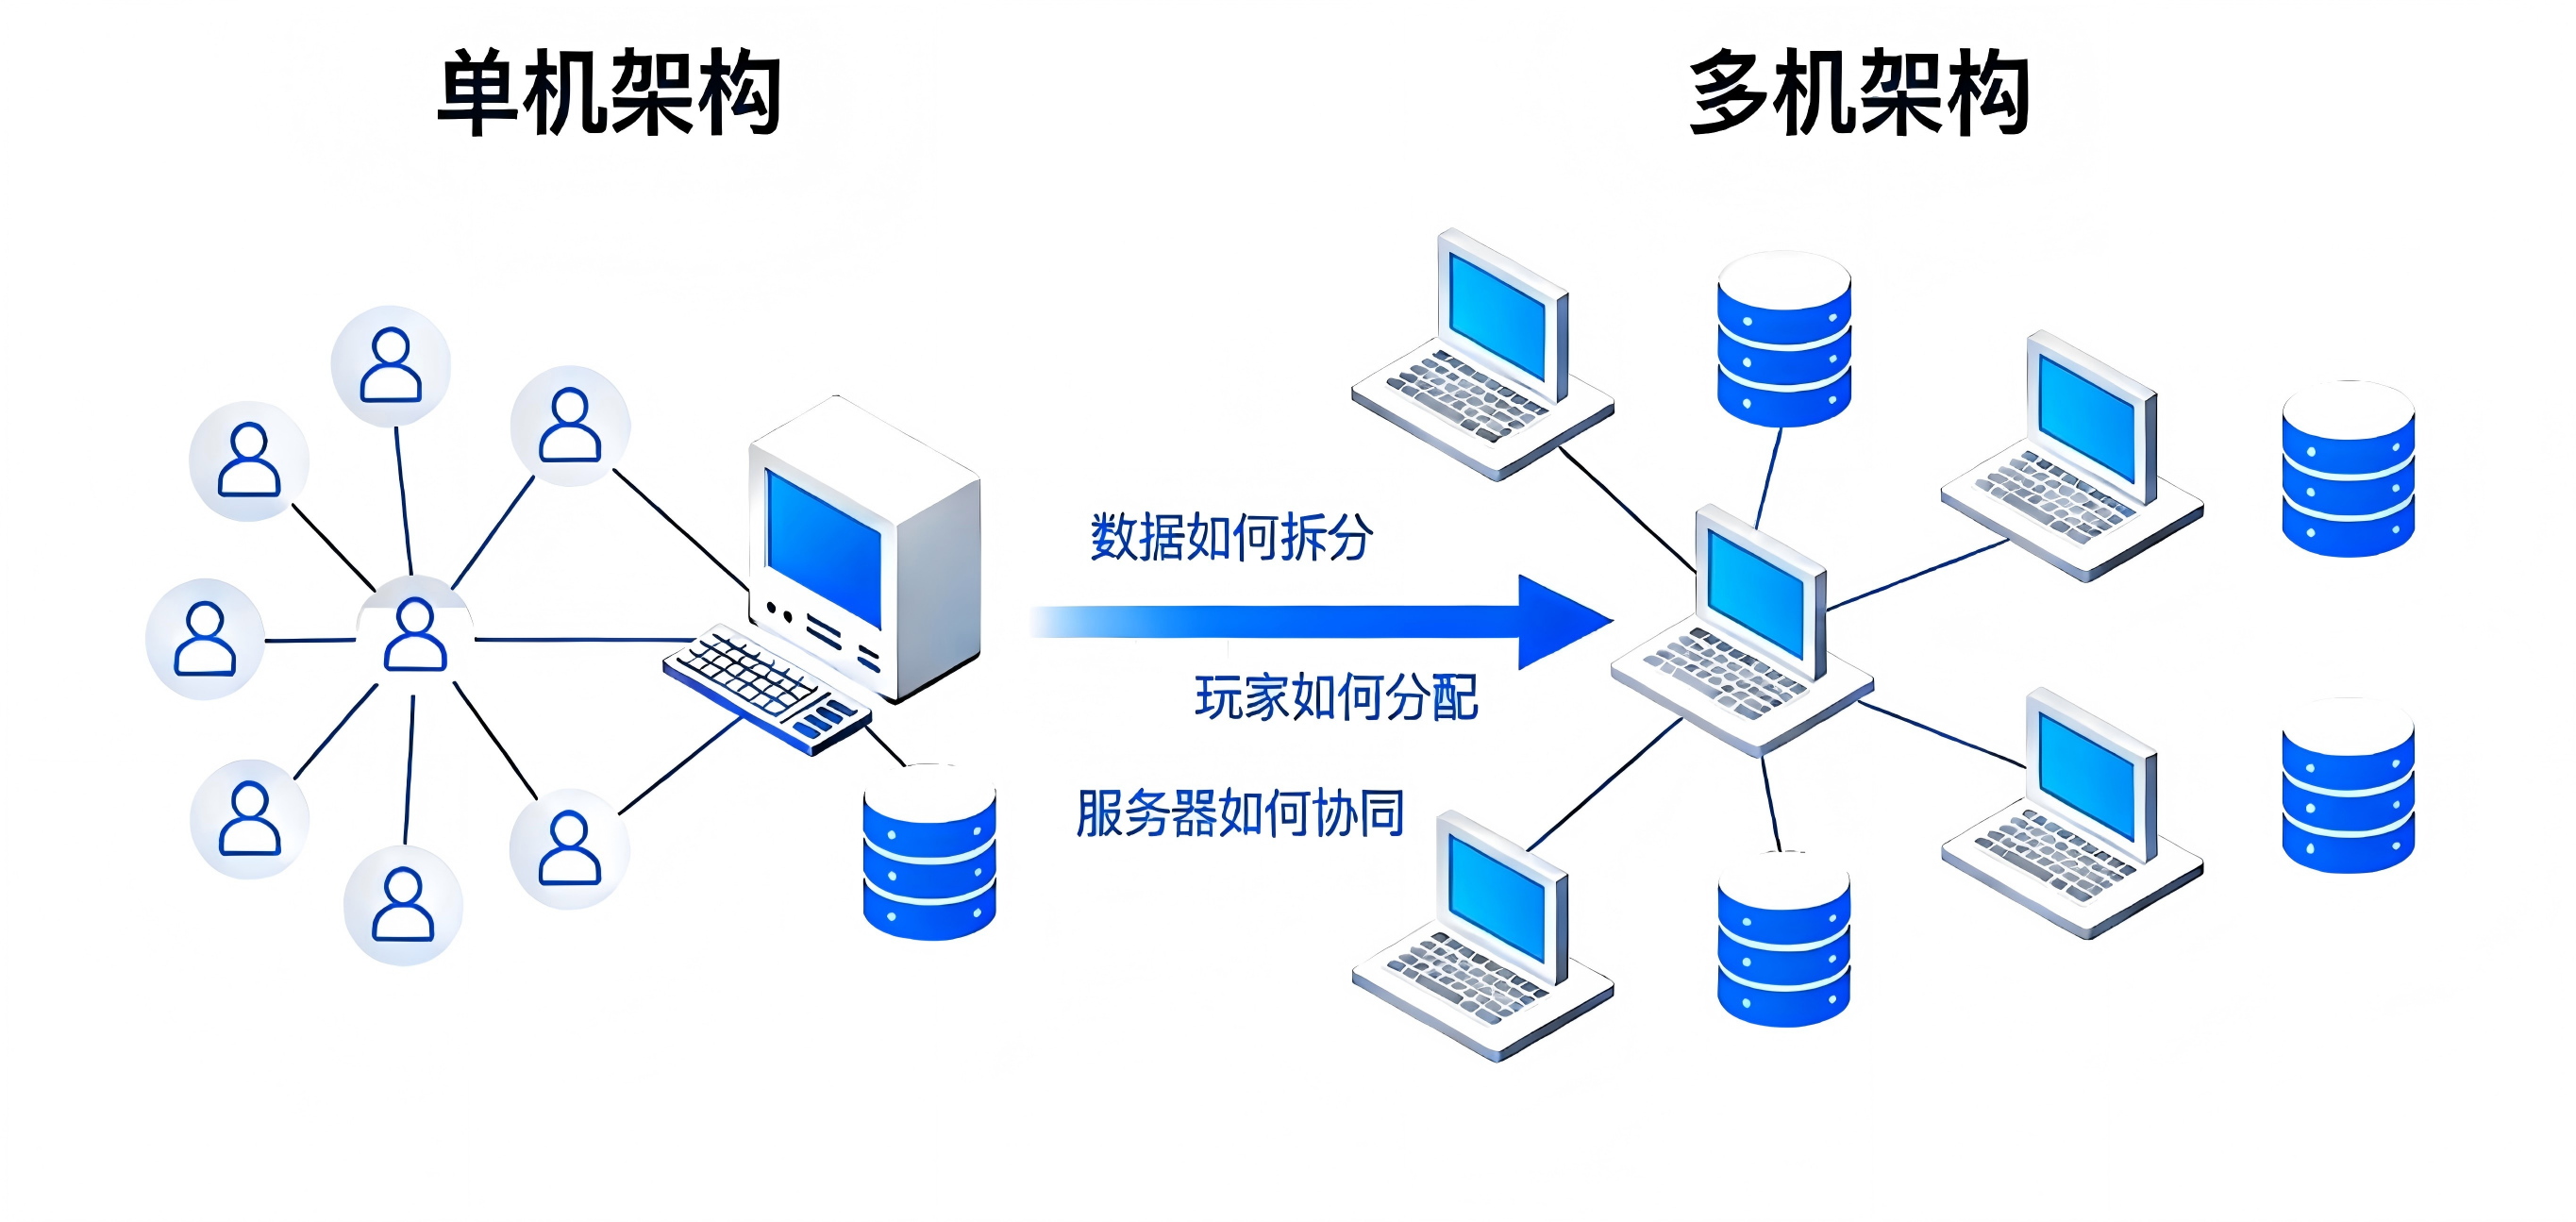
\includegraphics[width=1\linewidth]{figures/sec4/4-1.png}
    % 图片描述：展示从单机到多机架构的演进示意图
    % 左侧：单机架构，一个应用服务器连接一个数据库，所有玩家连接到这一个服务器
    % 右侧：多机架构，多个应用服务器，可能共享数据库或使用独立数据库
    % 用箭头标注出三个核心问题：数据如何拆分、玩家如何分配、服务器如何协同
    \caption{从单机到多机架构的演进与核心挑战}
    \label{fig:single_to_multi_server}
\end{figure}

这三个问题——数据放在哪里、玩家如何分配、不同服务器如何协同——构成了从单机到多机演进过程中必须解决的核心挑战。它们彼此关联、相互影响，形成了一个复杂的技术网络。数据的存放方式会影响查询效率，进而影响负载均衡的策略；负载均衡的效果会影响各服务器的压力分布，进而影响跨服交互的设计；跨服交互的实现方式又会对数据一致性提出新的要求，进而影响数据存储的架构选择。这就是为什么"加机器"这个看似简单的想法，在实际落地时会引发一系列连锁反应。

更深层次地说，从单机到多机的演进，本质上是从"集中式架构"到"分布式架构"的转变。在集中式架构中，所有的状态、所有的决策、所有的数据都集中在一个地方，系统的行为是确定的、可预测的。但在分布式架构中，状态被分散到多台机器上，每台机器都有自己的"局部视角"，它们需要通过网络通信来协调彼此的行为。网络通信是不可靠的——消息可能延迟、可能丢失、可能乱序到达；机器也是不可靠的——随时可能崩溃、重启、断网。在这样的环境下，如何确保系统整体上仍然能够正确、一致地运行，就成了分布式系统设计的核心挑战。

本章的目标，就是带领大家系统地理解和解决这些挑战。我们将从最基础、也是最关键的三个问题出发，将整章拆分为三个循序渐进的小节。第一节，我们会详细讲解"如何拆分数据"，介绍数据库分片的核心概念、常见策略，以及分片后会遇到的查询和事务问题；第二节，我们会深入探讨"如何分配玩家与负载"，从最简单的轮询策略开始，逐步引入动态调度、健康检查等机制，帮助大家理解负载均衡的完整体系；第三节，我们会通过一个具体的"跨服擂台"案例，把前两节学到的抽象概念织进一个完整的玩法场景之中，让大家亲身体验分布式环境下的跨服交互是如何设计和实现的。

通过这三个小节的学习，大家不仅能够掌握分布式游戏服务器的基础架构技术，更重要的是，能够建立起一套分布式系统思维——学会在设计任何涉及多台机器协同工作的系统时，自觉地去思考数据如何分布、负载如何均衡、节点如何协调这些根本性的问题。这种思维方式，不仅适用于游戏服务器，也适用于任何大规模的分布式应用系统。


\subsection{数据库分片：突破单机存储的容量上限}

回顾第三章，我们为单机服务器建立了Redis+PostgreSQL的分层存储架构：Redis承载高频热数据（在线状态、实时位置、排行榜），PostgreSQL持久化低频冷数据（账户信息、历史战绩、装备配置），两者通过写穿、写回、失效更新三种策略协同工作。在单机阶段，这套架构运行良好——一个Redis实例加一个PostgreSQL实例，足以支撑数百到数千名玩家的并发访问。

然而，当玩家规模从数千增长到数万乃至数十万时，这套单机数据层会在两个方向上同时触及天花板：PostgreSQL的磁盘I/O和连接数达到上限，查询延迟急剧恶化；Redis的内存容量不足以容纳所有在线玩家的热数据，开始频繁淘汰缓存导致穿透到数据库。此时，单纯的纵向扩展（换更大的机器）已经无法解决问题，我们必须将数据层从单实例拆分为多实例——这就是数据库分片的由来。本节将首先讨论PostgreSQL的分片策略，随后在本小节末尾说明Redis缓存层如何同步完成分布式演进。

当游戏还停留在单机阶段时，数据层的世界是简单而直观的：所有玩家的账号、角色、战斗记录，都躺在同一个数据库实例里，应用服务器只要连上这一个地址，就可以查到任何一个玩家的所有信息。在这个阶段，开发者更多关注的是"如何把这一个数据库调优到足够扛打"——加索引、调连接池、做缓存；但随着玩家规模上升，这个"一个数据库"慢慢变成了游戏世界里最脆弱的一块地基。

在深入讨论每一个具体问题之前，有必要先建立一个整体的架构视图，
下图展示了本节所涉及的数据分片体系的全貌。
整个体系自上而下分为三个层次：最上层是游戏应用服务器，它是所有数据库请求的发起方；
中间层是分片路由层，它是整个分片体系的神经中枢，负责接收来自应用服务器的请求，
根据请求中携带的玩家 ID 和预先配置的分片规则，计算出目标分片编号，
再将请求精准转发到对应的数据库实例；最下层是由多个 PostgreSQL 分片实例组成的存储层，
每个分片只负责全量玩家数据的一个子集，各分片之间相互独立，互不干扰。
与 PostgreSQL 分片层并列运行的，是 Redis 缓存集群，
它以相同的分片逻辑将热数据键空间拆分到多个 Redis 节点上，
承载在线状态、实时位置、排行榜片段等高频访问数据，与冷数据层共同构成完整的分布式数据层。

\begin{figure}[H]
    \centering
    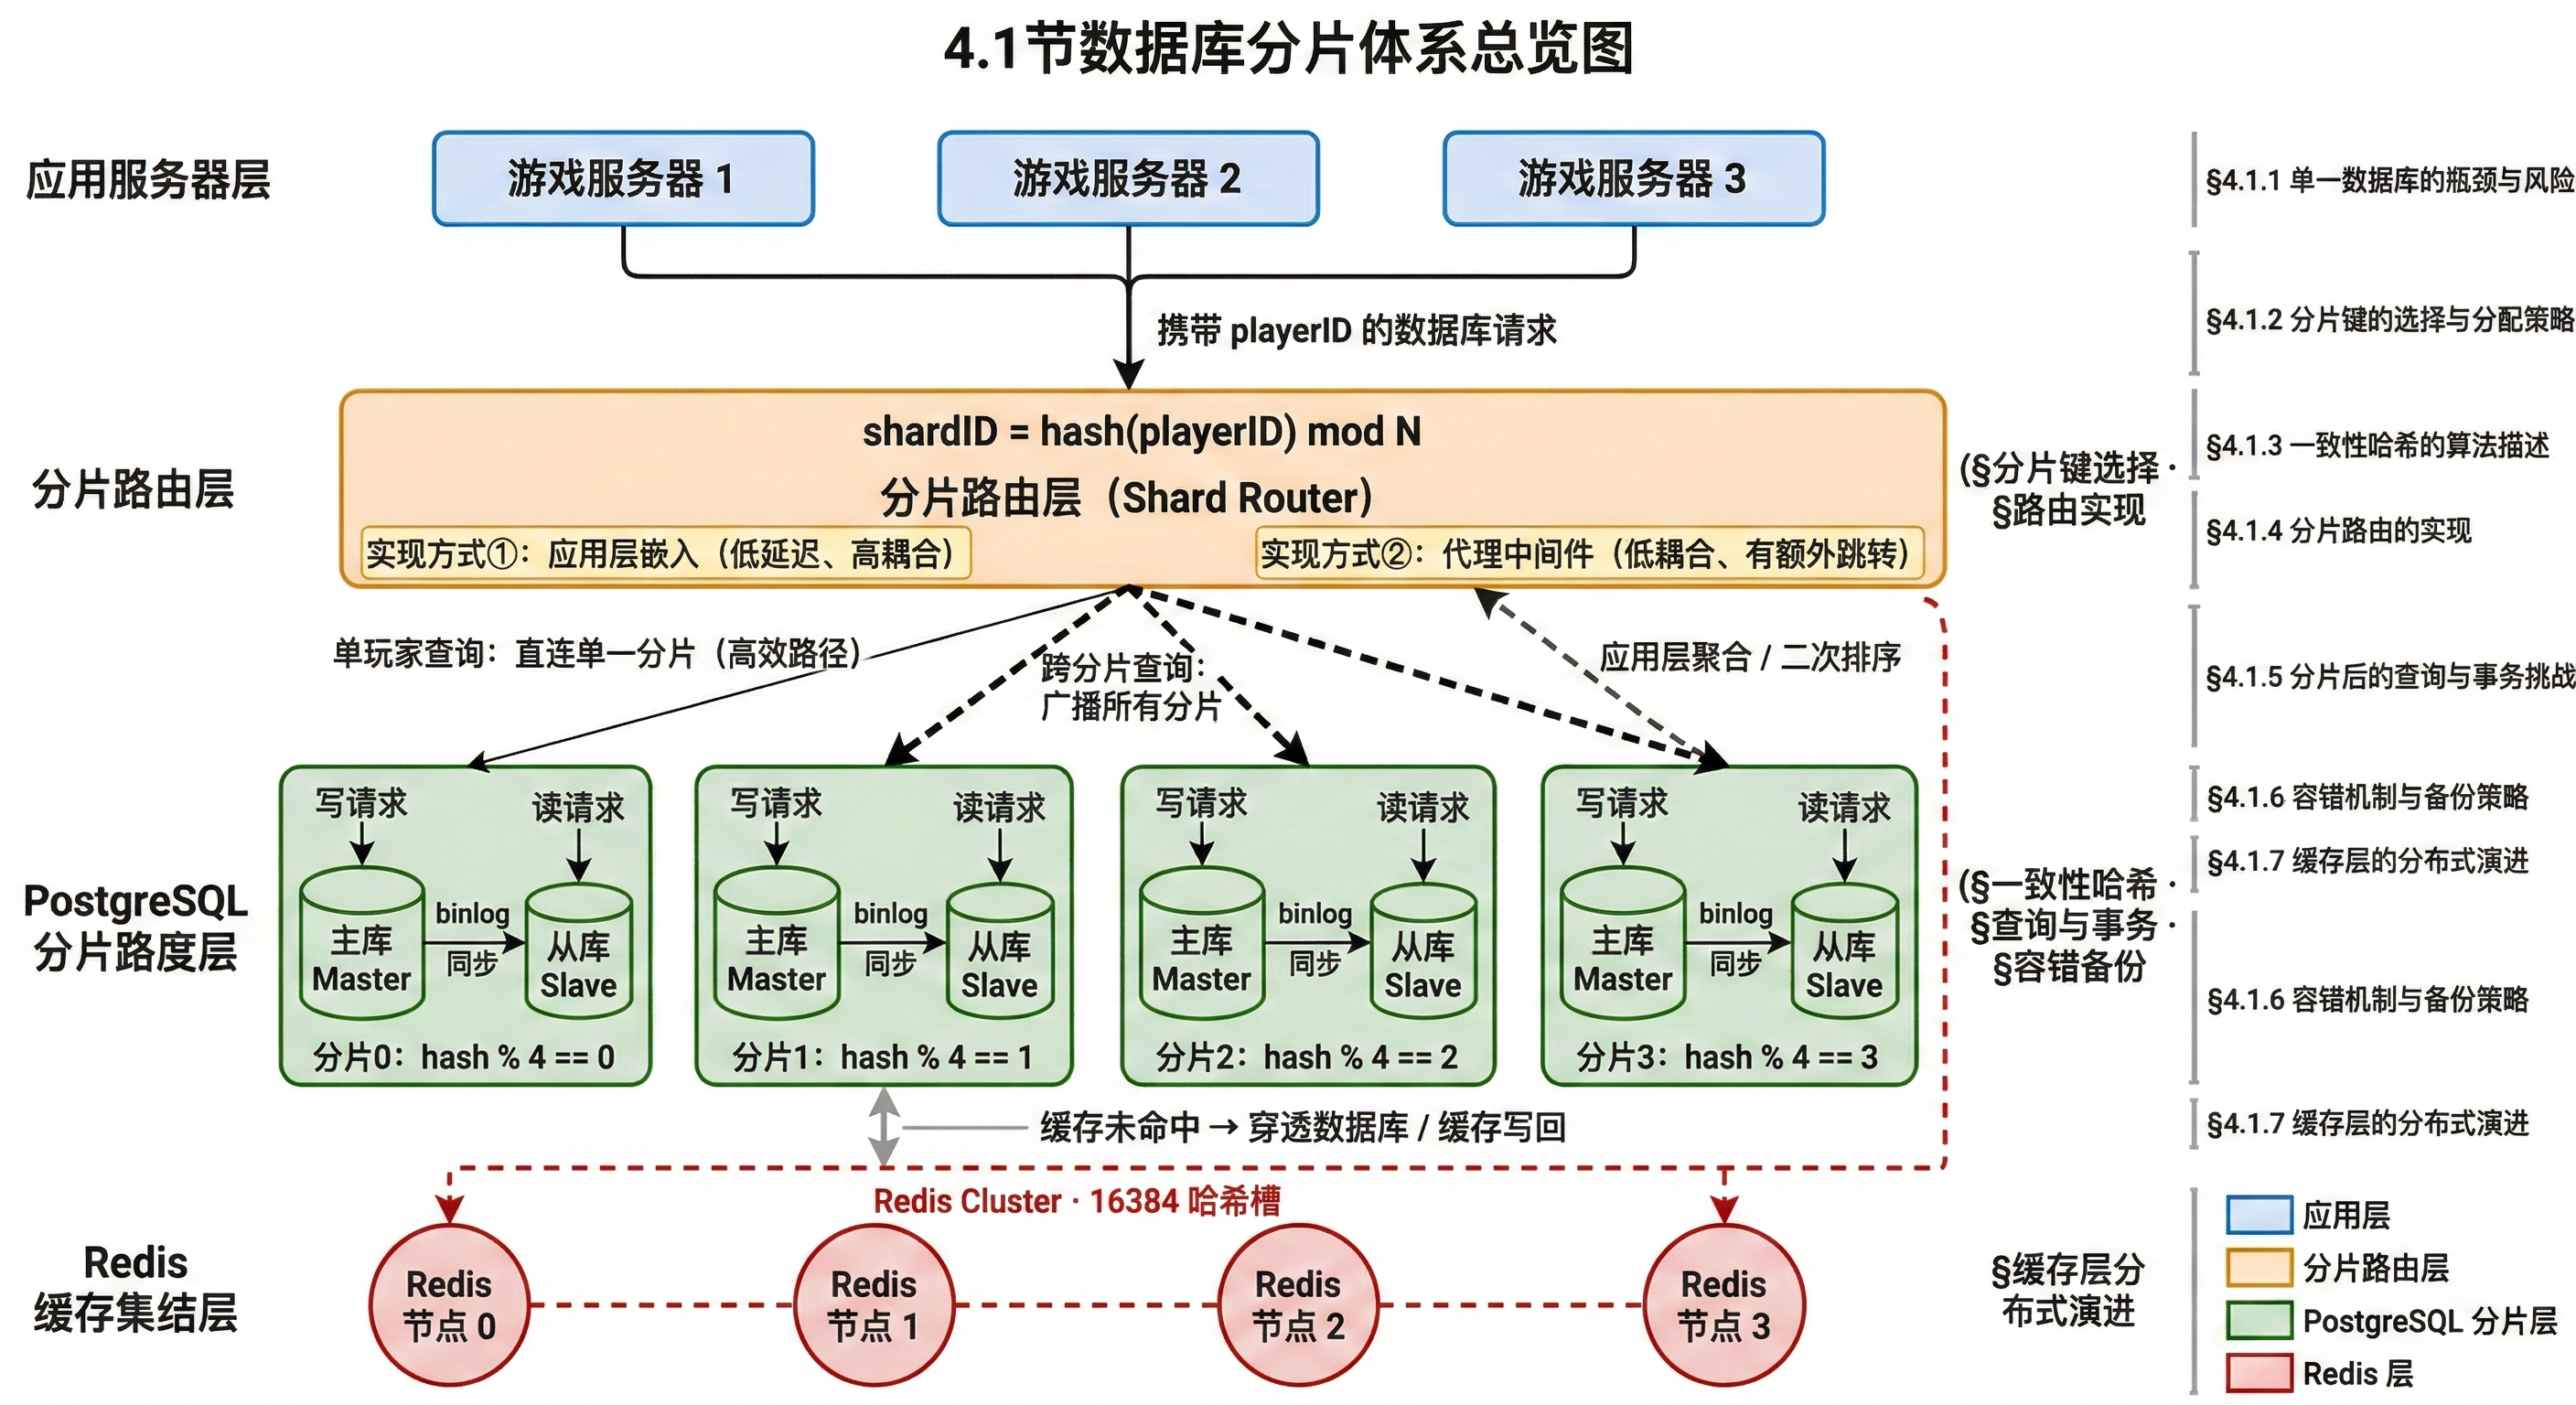
\includegraphics[width=1\linewidth]{figures/sec4/4-1-1.png}
    \caption{数据库分片体系总览}
\end{figure}

这张图揭示了整个分片体系的两条核心请求链路。
第一条是单玩家查询链路：请求携带玩家 ID 进入路由层，
路由层经过一次哈希计算便能唯一确定目标分片，请求直达单个数据库节点，
全程无需跨节点协调，这是分片架构在正常访问路径上高效运作的根本原因。
第二条是跨分片链路：当查询不能通过分片键唯一定位时——
例如全服战力排行榜需要聚合所有分片的数据——
路由层必须将请求广播到全部分片，由各分片分别执行子查询，
再由应用层将各分片的局部结果合并排序后返回最终答案；
分布式事务同样属于跨分片链路的范畴，需要通过两阶段提交协议或业务层异步化来保障操作的原子性。
这两条链路的效率差异，正是本节反复强调"尽量将查询限制在单一分片内"这一设计原则的根源。

本节各小节的讨论便是沿着这张图从上到下、由浅入深地逐层展开的。
首先从单一数据库所面临的硬件天花板和单点故障风险出发，说明为什么必须走向水平拆分；随后讨论分片键的选择与三种分配策略——范围分片、哈希分片、一致性哈希——之间的权衡，
以及一致性哈希如何通过哈希环和虚拟节点将扩容时的数据迁移量控制在局部区间；接着说明路由层的两种实现方式，即应用层嵌入路由逻辑与引入代理中间件各自的适用场景；
然后面对分片后不可回避的两类技术难题，即跨分片聚合查询的效率损耗，以及跨分片事务的一致性保障与业务层规避策略；
再之后讨论每个分片内部的主从复制架构、定期备份机制与恢复演练，构建完整的容错体系；最后将视角切换到 Redis 缓存集群，说明热数据层如何完成与冷数据层对称的分布式演进，补全整个数据层的水平扩展图景。
%理解了这张总览图中各组件的角色与两条链路的走向，再阅读后续各小节的技术细节，便能始终清楚自己在整个分片体系中所处的位置。


\subsubsection{单一数据库的瓶颈与风险}

从最直观的角度看，单一数据库的瓶颈首先体现在硬件资源的天花板上。一台数据库服务器的 CPU 核心数、内存容量、磁盘 I/O 吞吐率都是有限的，当并发查询请求超过这些硬件资源所能承载的上限时，系统必然出现性能下降。可以想象这样一个场景：新版本上线，大量玩家同时登录、创建角色、领取奖励，这些操作最后都会汇聚到同一个数据库。一开始只是响应时间从正常的 50 毫秒逐渐攀升到 200 毫秒，玩家可能还察觉不到明显差异；但随着负载继续增加，响应时间可能突破 1 秒甚至更长，出现间歇性超时，部分玩家会看到"网络连接失败"的提示；最严重的情况下，数据库会直接触发过载保护机制，拒绝接受新的连接请求，导致大量玩家无法登录。

即使通过垂直扩展——也就是给这台机器加更多的 CPU、更大的内存——能够在一定程度上缓解压力，这条路终归是有尽头的。一台配置了 64 核 CPU、512GB 内存的高端数据库服务器，成本可能是普通服务器的十倍甚至更高，但性能提升往往达不到十倍。更关键的是，单台机器的物理极限也不可能无限突破：内存总线带宽、磁盘 I/O 吞吐量、网络接口速度都有上限，当这些指标逼近硬件极限时，再怎么堆钱也无法继续提升。

更深层的问题在于风险集中。当所有玩家的核心数据都存放在同一台数据库上时，这台机器的任何故障都会演化为全局灾难。硬盘损坏、网络中断、操作系统崩溃，任何一个环节出问题，都意味着整个游戏世界暂时失去了"记忆中枢"。虽然可以通过定期备份来降低数据永久丢失的风险，但备份无法解决实时可用性的问题——即使我们有昨天晚上的完整备份，当数据库在今天中午崩溃时，从发现故障、启动恢复流程、重新加载数据到服务恢复，整个过程可能需要数小时甚至更长时间，这对于一个需要 24 小时不间断运行的游戏服务来说是不可接受的。

从这两个角度出发，数据库拆分的核心动机便呼之欲出：通过将数据分散存储到多台独立的数据库实例上，一方面可以突破单机硬件资源的天花板，实现存储容量和查询吞吐量的水平扩展；另一方面，可以将风险分散开来，使得某一台数据库的故障只影响其所负责的那一部分玩家，而不会拖垮整个游戏世界。在分布式系统的术语中，这种将数据按照某种规则拆分到多台机器上的技术，被称为"数据库分片"（Database Sharding）。

\begin{figure}[htbp]
    \centering
    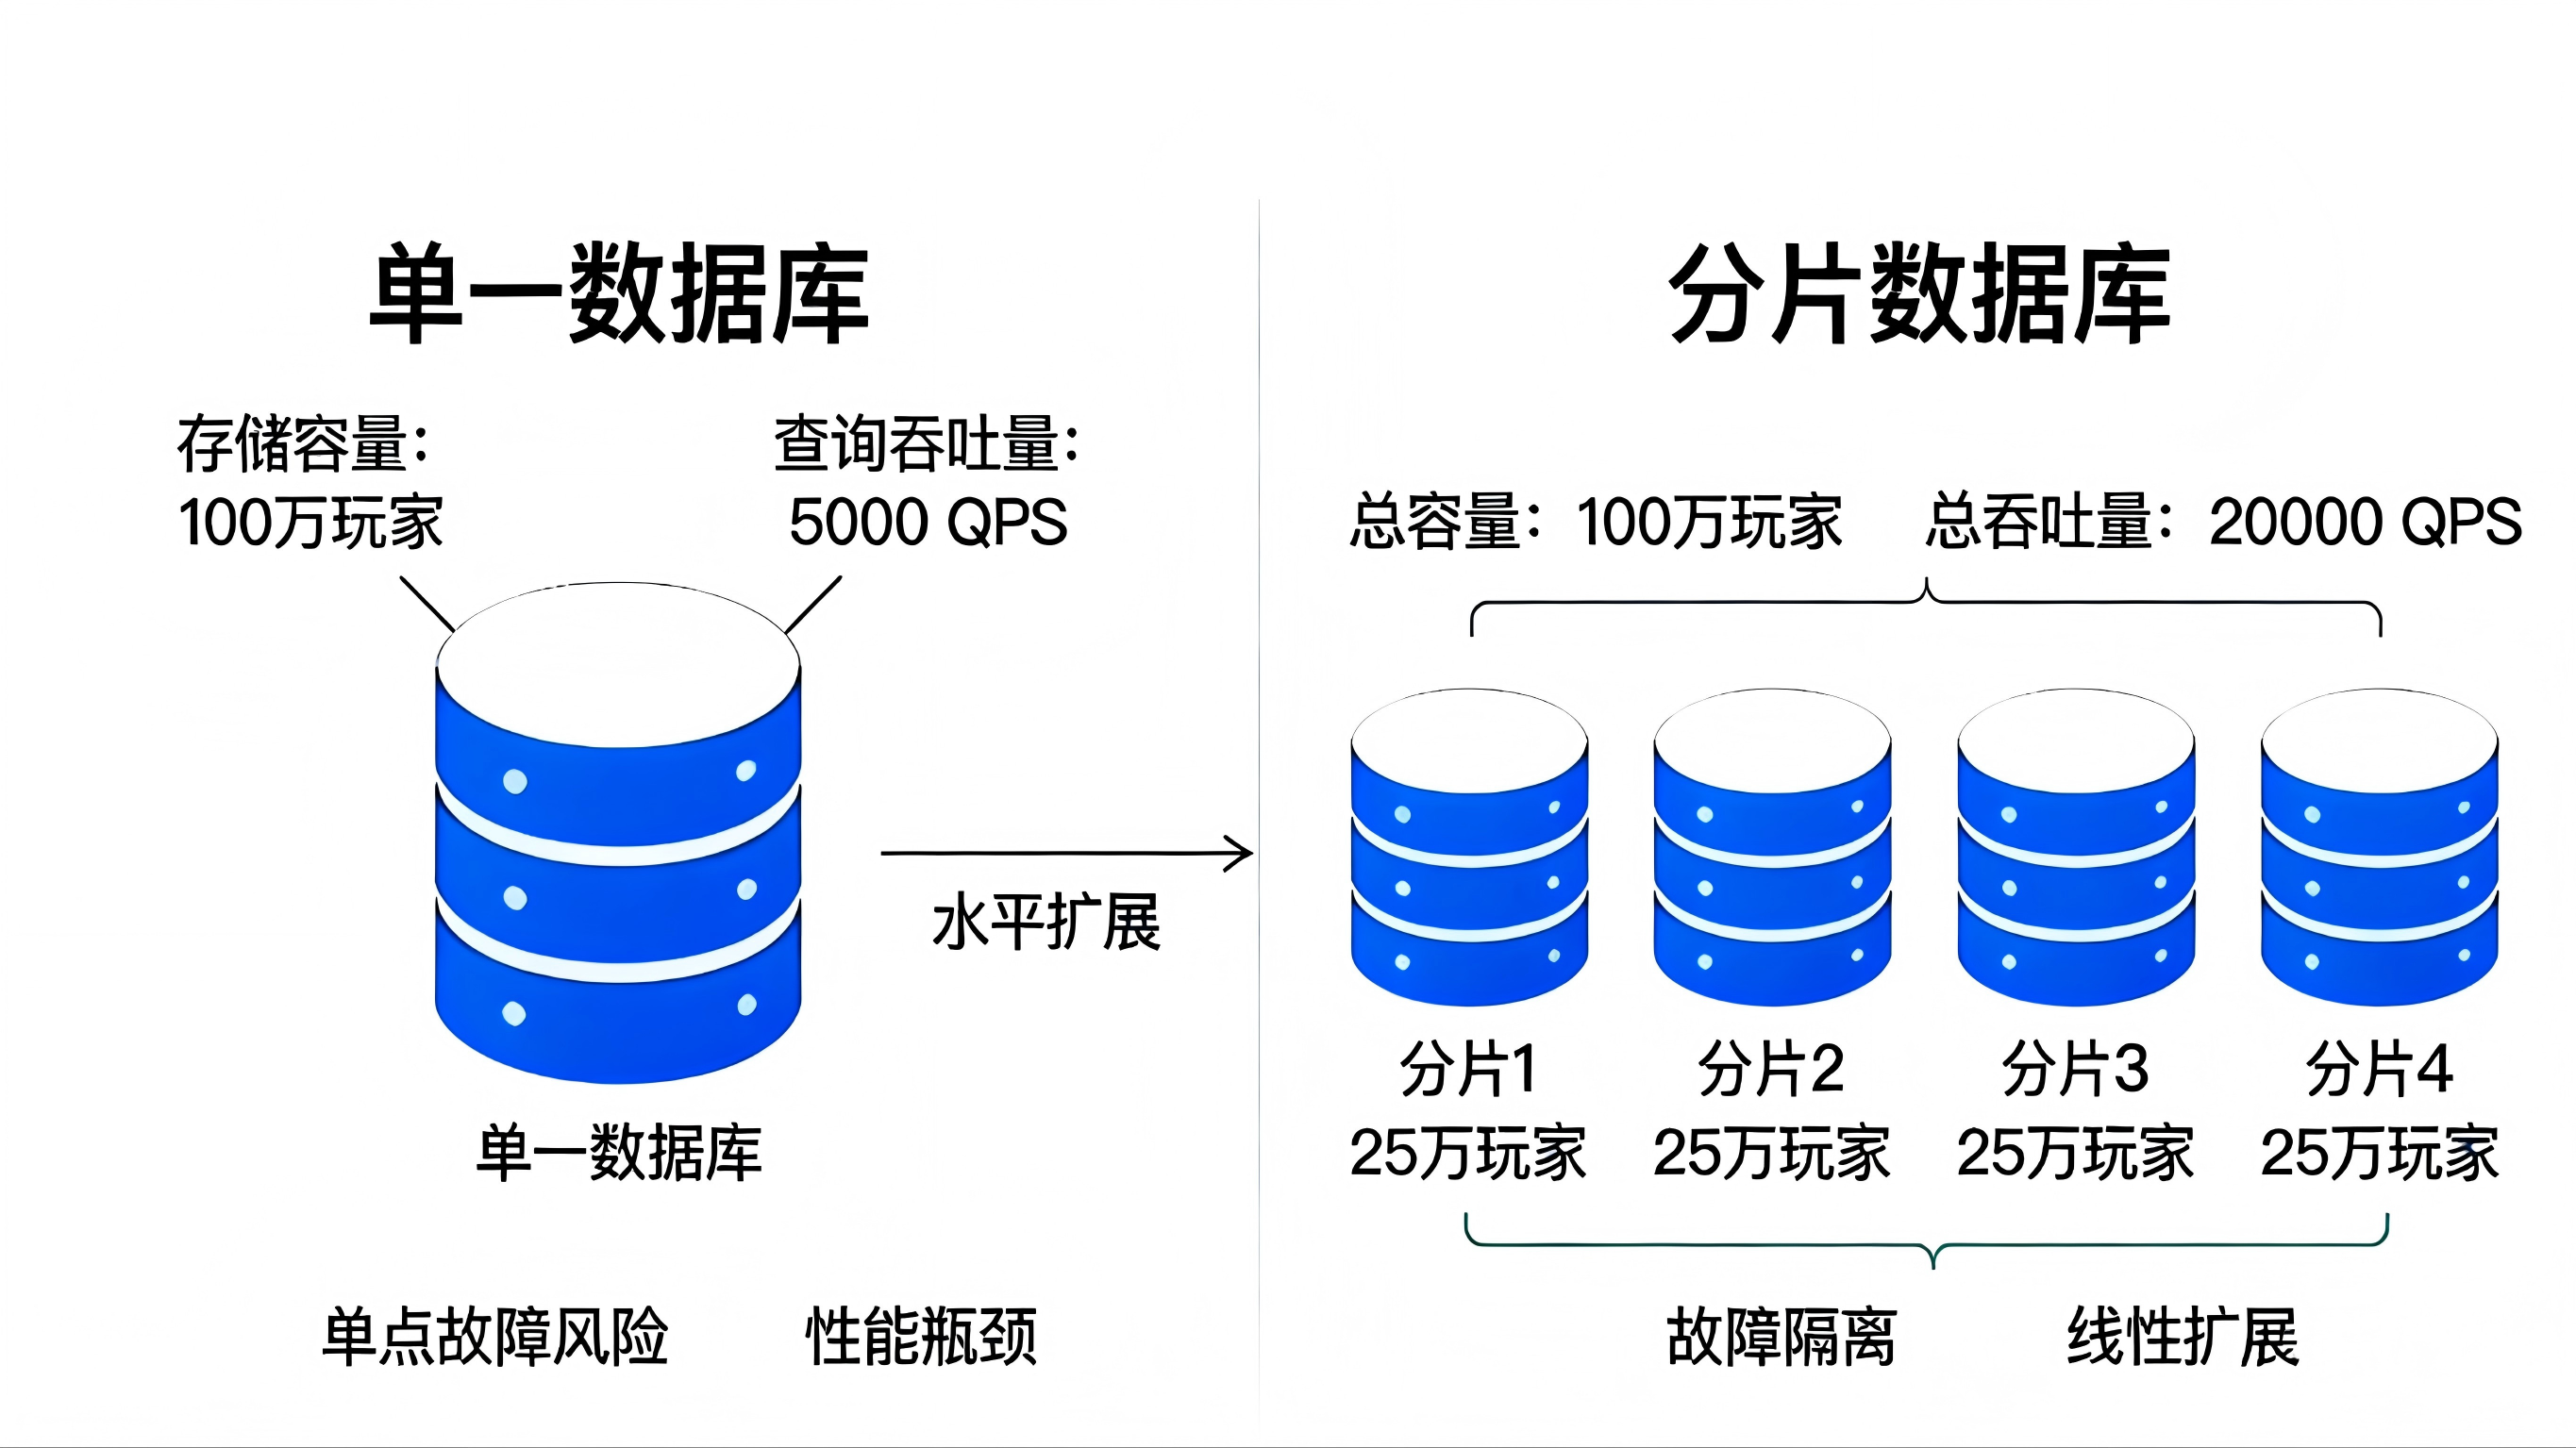
\includegraphics[width=1\linewidth]{figures/sec4/4-2.png}
    % 图片描述：单一数据库vs分片数据库的对比示意图
    % 左侧：单一数据库场景
    %   - 一个大的圆柱形数据库图标，标注"单一数据库"
    %   - 上方标注"存储容量：100万玩家"、"查询吞吐量：5000 QPS"
    %   - 下方用红色警告图标标注"单点故障风险"、"性能瓶颈"
    % 右侧：分片数据库场景（4个分片）
    %   - 四个较小的圆柱形数据库图标并排，分别标注"分片1"、"分片2"、"分片3"、"分片4"
    %   - 每个分片下方标注"25万玩家"
    %   - 上方汇总标注"总容量：100万玩家"、"总吞吐量：20000 QPS"
    %   - 下方用绿色对勾标注"故障隔离"、"线性扩展"
    % 中间用箭头连接，箭头上标注"水平扩展"
    % 所有文字使用简体中文，采用黑色粗体无衬线字体
    \caption{单一数据库与分片数据库的容量与风险对比}
    \label{fig:database_sharding_comparison}
\end{figure}

\subsubsection{分片键的选择与分配策略}

要理解数据库分片，需要先明确一个核心概念：分片键（Sharding Key）。分片键是用来决定某一条数据应该被分配到哪个数据库实例的关键字段。在游戏服务器的场景下，最自然的选择是以玩家 ID 作为分片键。原因很简单：首先，玩家 ID 在整个系统中是唯一的，每个玩家对应一个固定的 ID，这个 ID 在玩家整个生命周期内都不会改变，不会出现像昵称那样可能被修改的情况；其次，游戏中的绝大多数查询操作都是围绕玩家 ID 展开的——查询某个玩家的角色信息、战斗记录、背包物品等，都需要先知道玩家 ID。如果用玩家 ID 作为分片键，那么查询单个玩家的数据时，只需要根据 ID 定位到一个具体的数据库实例，不需要在多个实例之间查找。

确定了用玩家 ID 作为分片键之后，接下来需要设计具体的分配规则。这个规则需要回答一个简单但关键的问题：给定一个玩家 ID，它的数据应该存放在哪个数据库实例中？不同的分配规则会带来不同的特性和权衡，我们逐一分析三种常见的方案。

第一种方案是范围分片（Range-based Sharding）。这是最直观的一种方式：按照玩家 ID 的数值范围来划分数据。假设我们有三个数据库实例，可以这样分配：ID 从 1 到 1,000,000 的玩家存放在第一个数据库（分片 0），ID 从 1,000,001 到 2,000,000 的存放在第二个数据库（分片 1），ID 从 2,000,001 以上的存放在第三个数据库（分片 2）。这种方式的优点在于规则简单明了，容易理解和管理。当需要查询某个玩家的数据时，只需要简单地判断 ID 落在哪个区间即可。而且，如果需要扩容，只需要调整最后一个区间的边界，新增一个数据库实例来承接新的 ID 范围即可。

但范围分片也有一个明显的隐患——负载热点问题。如果玩家注册在时间上非常集中，比如游戏刚上线或举办大型活动期间，短时间内会有大量新玩家涌入，他们会被连续分配到相邻的 ID 区间。假设在一周内新注册了 50 万玩家，他们的 ID 都落在 2,000,001 到 2,500,000 这个范围内，全部被分配到分片 2。而这些新玩家往往是最活跃的——频繁登录、进行战斗、完成任务——导致分片 2 的负载远高于其他分片。这就像是一个不断向右延伸的队列，最右边的那一块总是最拥挤的。

% \begin{figure}[htbp]
%     \centering
%     % 图片描述：范围分片的热点问题示意图
%     % 横轴代表玩家ID范围（0到3,000,000），纵轴代表负载强度
%     % 三个区间分别用不同颜色柱状图表示：
%     %   - 分片0（ID 1-1,000,000）：绿色柱，高度较低，标注"老玩家，活跃度低"
%     %   - 分片1（ID 1,000,001-2,000,000）：黄色柱，高度中等，标注"中期玩家，活跃度中等"
%     %   - 分片2（ID 2,000,001以上）：红色柱，高度很高，标注"新玩家，活跃度高，形成热点"
%     % 在分片2上方标注红色警告标志和文字"负载热点"
%     % 所有文字使用简体中文
%     \caption{范围分片可能导致的负载热点问题}
%     \label{fig:range_sharding_hotspot}
% \end{figure}

为了避免这个问题，第二种方案是哈希分片（Hash-based Sharding）。具体做法是：对每个玩家 ID 执行一个固定的哈希运算，将结果对数据库实例数量取模，根据余数来决定数据存放的位置。用伪代码表示如下：

\begin{tcolorbox}[title=哈希分片的路由计算]
\begin{lstlisting}[
    language=go,
    basicstyle=\ttfamily\footnotesize,
    aboveskip=0pt, belowskip=0pt,
    lineskip=-1pt,
    commentstyle=\color{gray},
    keywordstyle=\color{blue}\bfseries,
    breaklines=true
]
// 假设有4个数据库分片
const numShards = 4

// 根据玩家ID计算目标分片
func getShardID(playerID int) int {
    // 对玩家ID执行哈希运算（这里用简单的取模代替）
    hash := playerID
    // 对分片数量取模，得到分片编号（0-3）
    shardID := hash % numShards
    return shardID
}

// 示例：不同玩家ID被分配到不同分片
// 玩家1 -> 分片1, 玩家2 -> 分片2, 玩家3 -> 分片3
// 玩家4 -> 分片0, 玩家5 -> 分片1, 玩家6 -> 分片2
// 即使ID连续，也会被打散到不同分片
\end{lstlisting}
\end{tcolorbox}

由于哈希函数的输出具有一定的随机性和均匀性，即使玩家 ID 在时间上连续注册（1, 2, 3, 4...），经过哈希和取模之后也会被打散到不同的数据库实例中。例如，玩家 ID 为 1、5、9、13 的会被分配到分片 1，玩家 ID 为 2、6、10、14 的会被分配到分片 2，以此类推。这样就有效避免了新玩家集中在某一个分片的问题，实现了负载的相对均衡。

\begin{figure}[htbp]
    \centering
    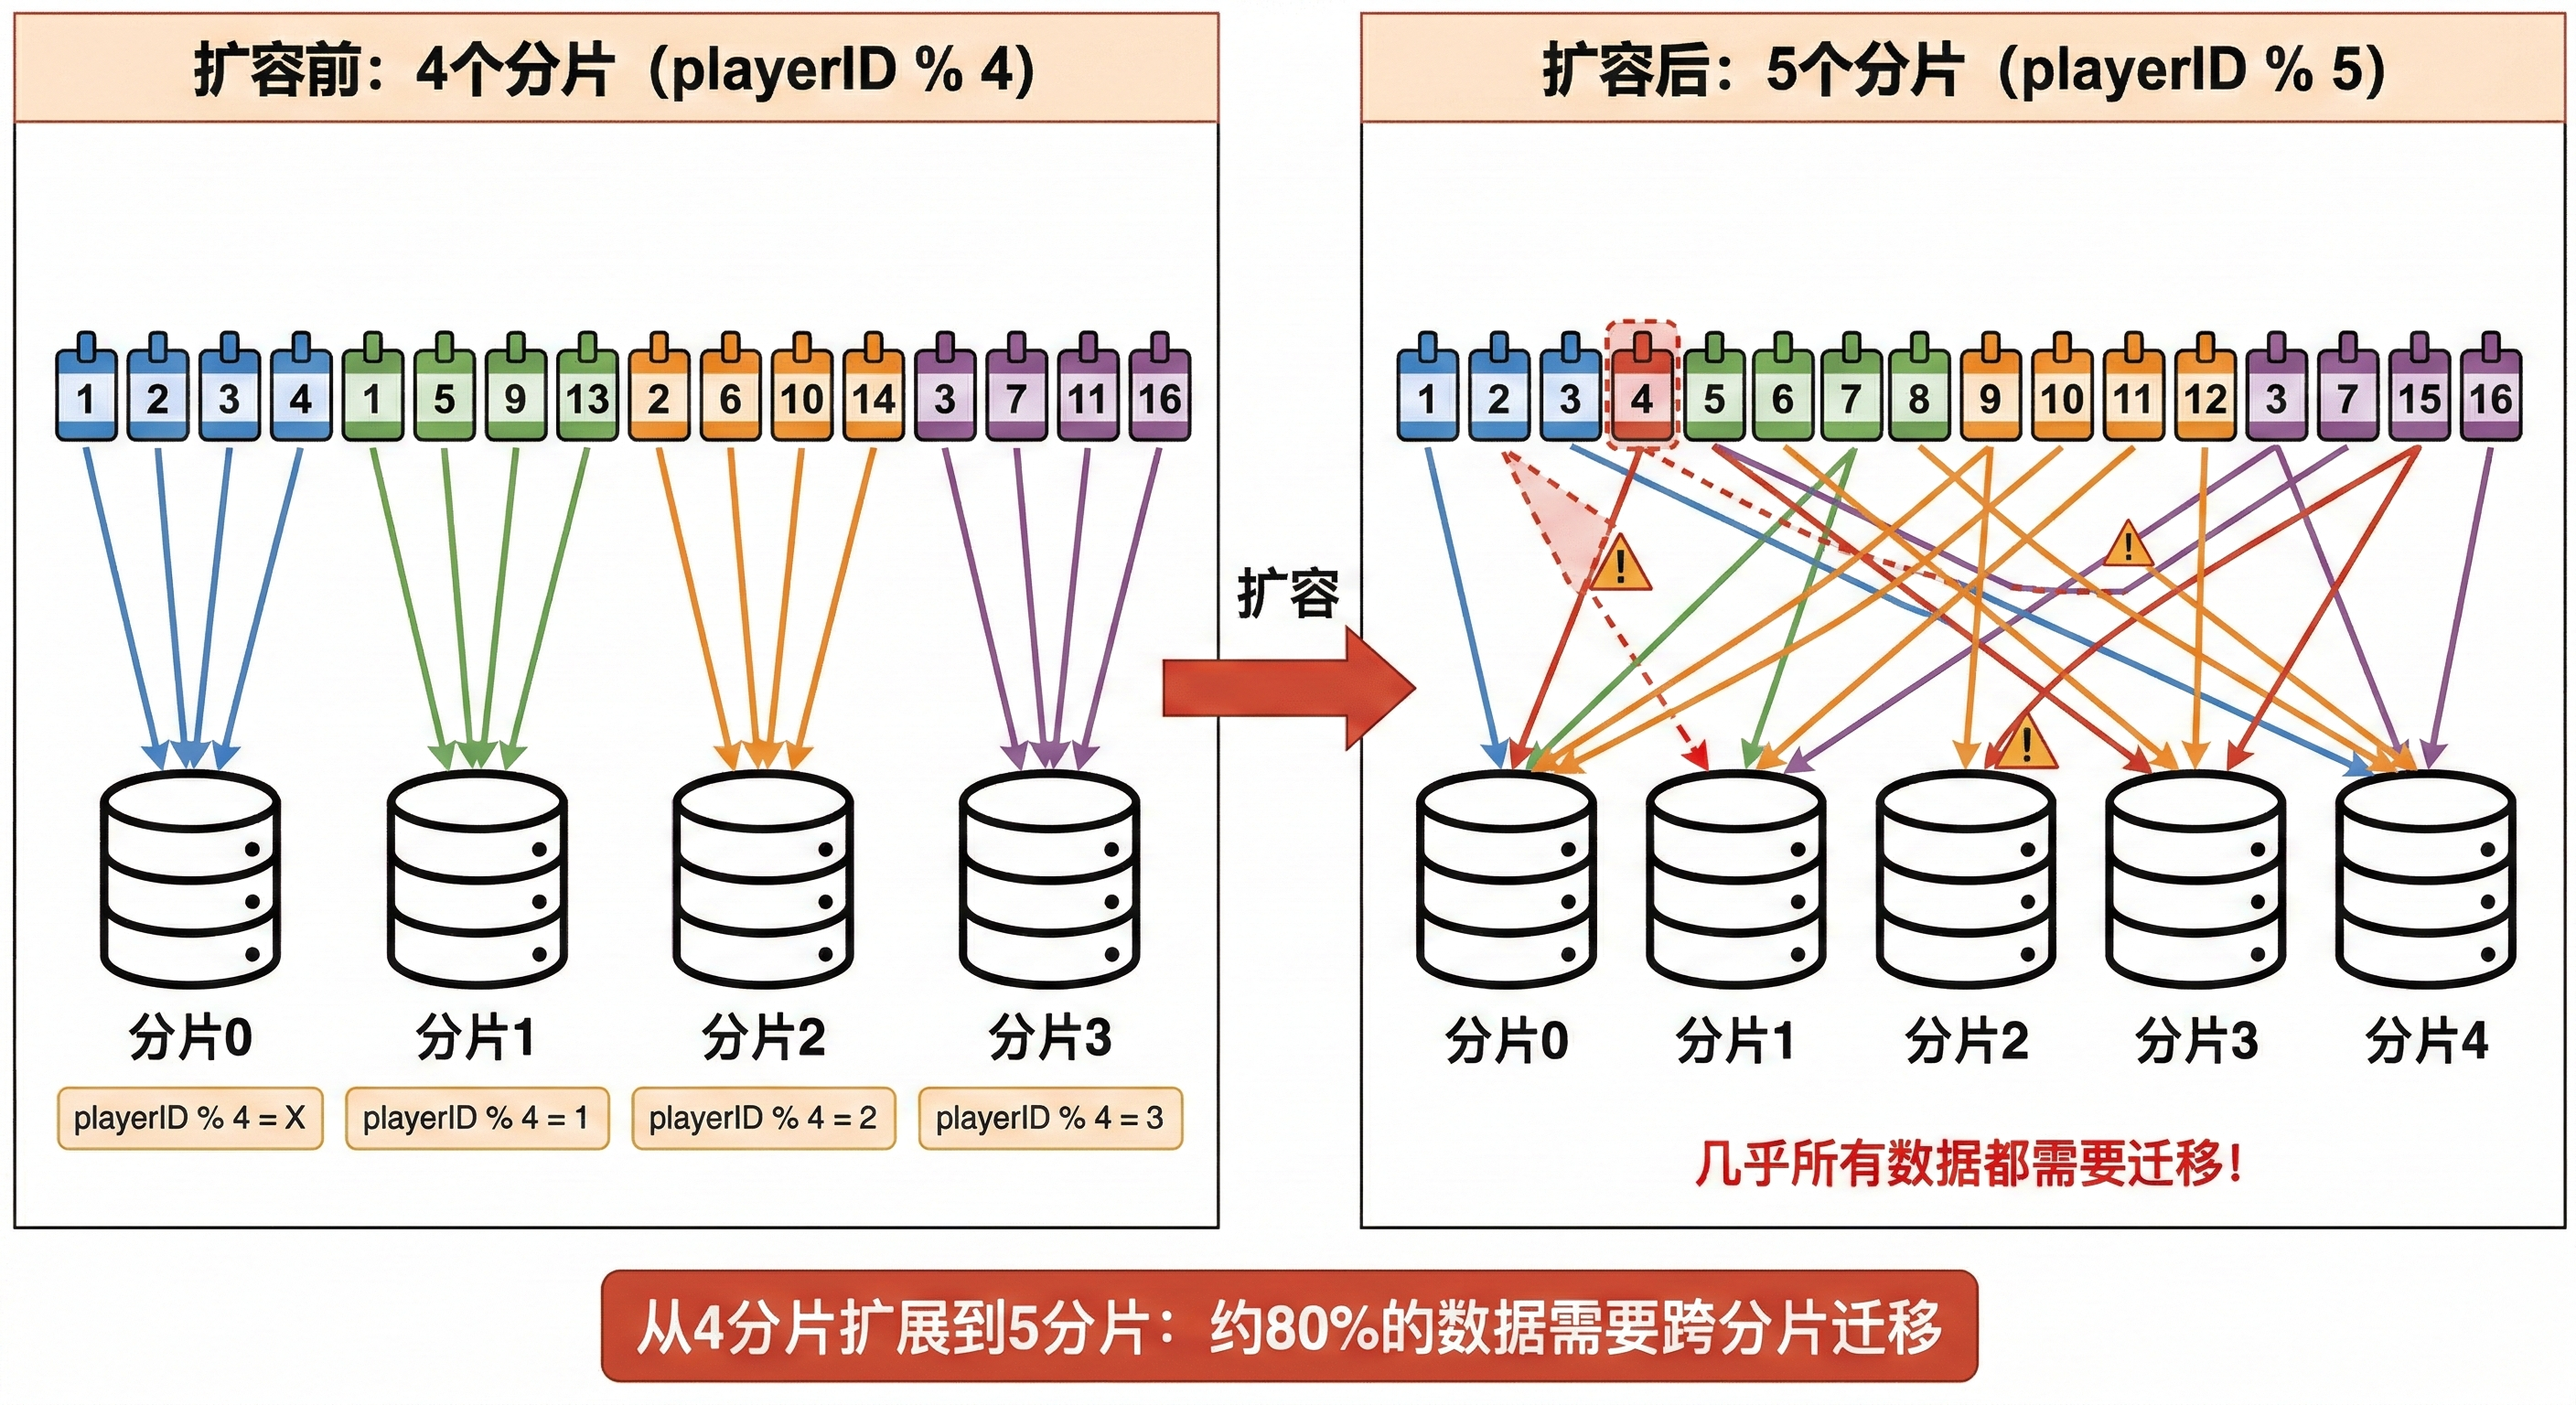
\includegraphics[width=1\linewidth]{figures/sec4/4-6-1.png}
    \caption{哈希分片扩容的数据迁移代价：从4个分片扩展到5个分片时，取模基数改变导致绝大多数玩家的分片归属发生变化，引发大规模数据迁移}
    \label{fig:consistent_hashing}
\end{figure}

但哈希分片也有自己的代价——扩容困难。当我们需要增加数据库实例数量时，比如从 4 个分片扩展到 5 个，取模的基数从 4 变成了 5，这意味着几乎所有玩家的哈希结果都会发生变化。原本 \texttt{playerID \% 4 = 1} 的玩家，现在 \texttt{playerID \% 5} 的结果可能变成 2 或 3 或其他值。这就要求我们重新计算每个玩家应该在哪个分片，并将大量数据从原分片迁移到新分片。对于一个拥有数百万玩家的游戏来说，这种大规模的数据迁移不仅耗时巨大，还可能在迁移过程中影响系统的可用性。

为了缓解扩容时的数据迁移问题，第三种方案是一致性哈希（Consistent Hashing）。一致性哈希的核心思想是将数据库实例和玩家 ID 都映射到一个虚拟的哈希环上——可以想象成一个钟表的表盘，刻度从 0 到 $2^{32}-1$（或其他上限值）。首先，我们将每个数据库实例通过哈希函数映射到环上的某个位置；然后，对于每个玩家 ID，也通过同样的哈希函数映射到环上的某个位置，再在环上顺时针寻找最近的数据库实例节点，这个节点就是该玩家数据存放的位置。

\begin{figure}[htbp]
    \centering
    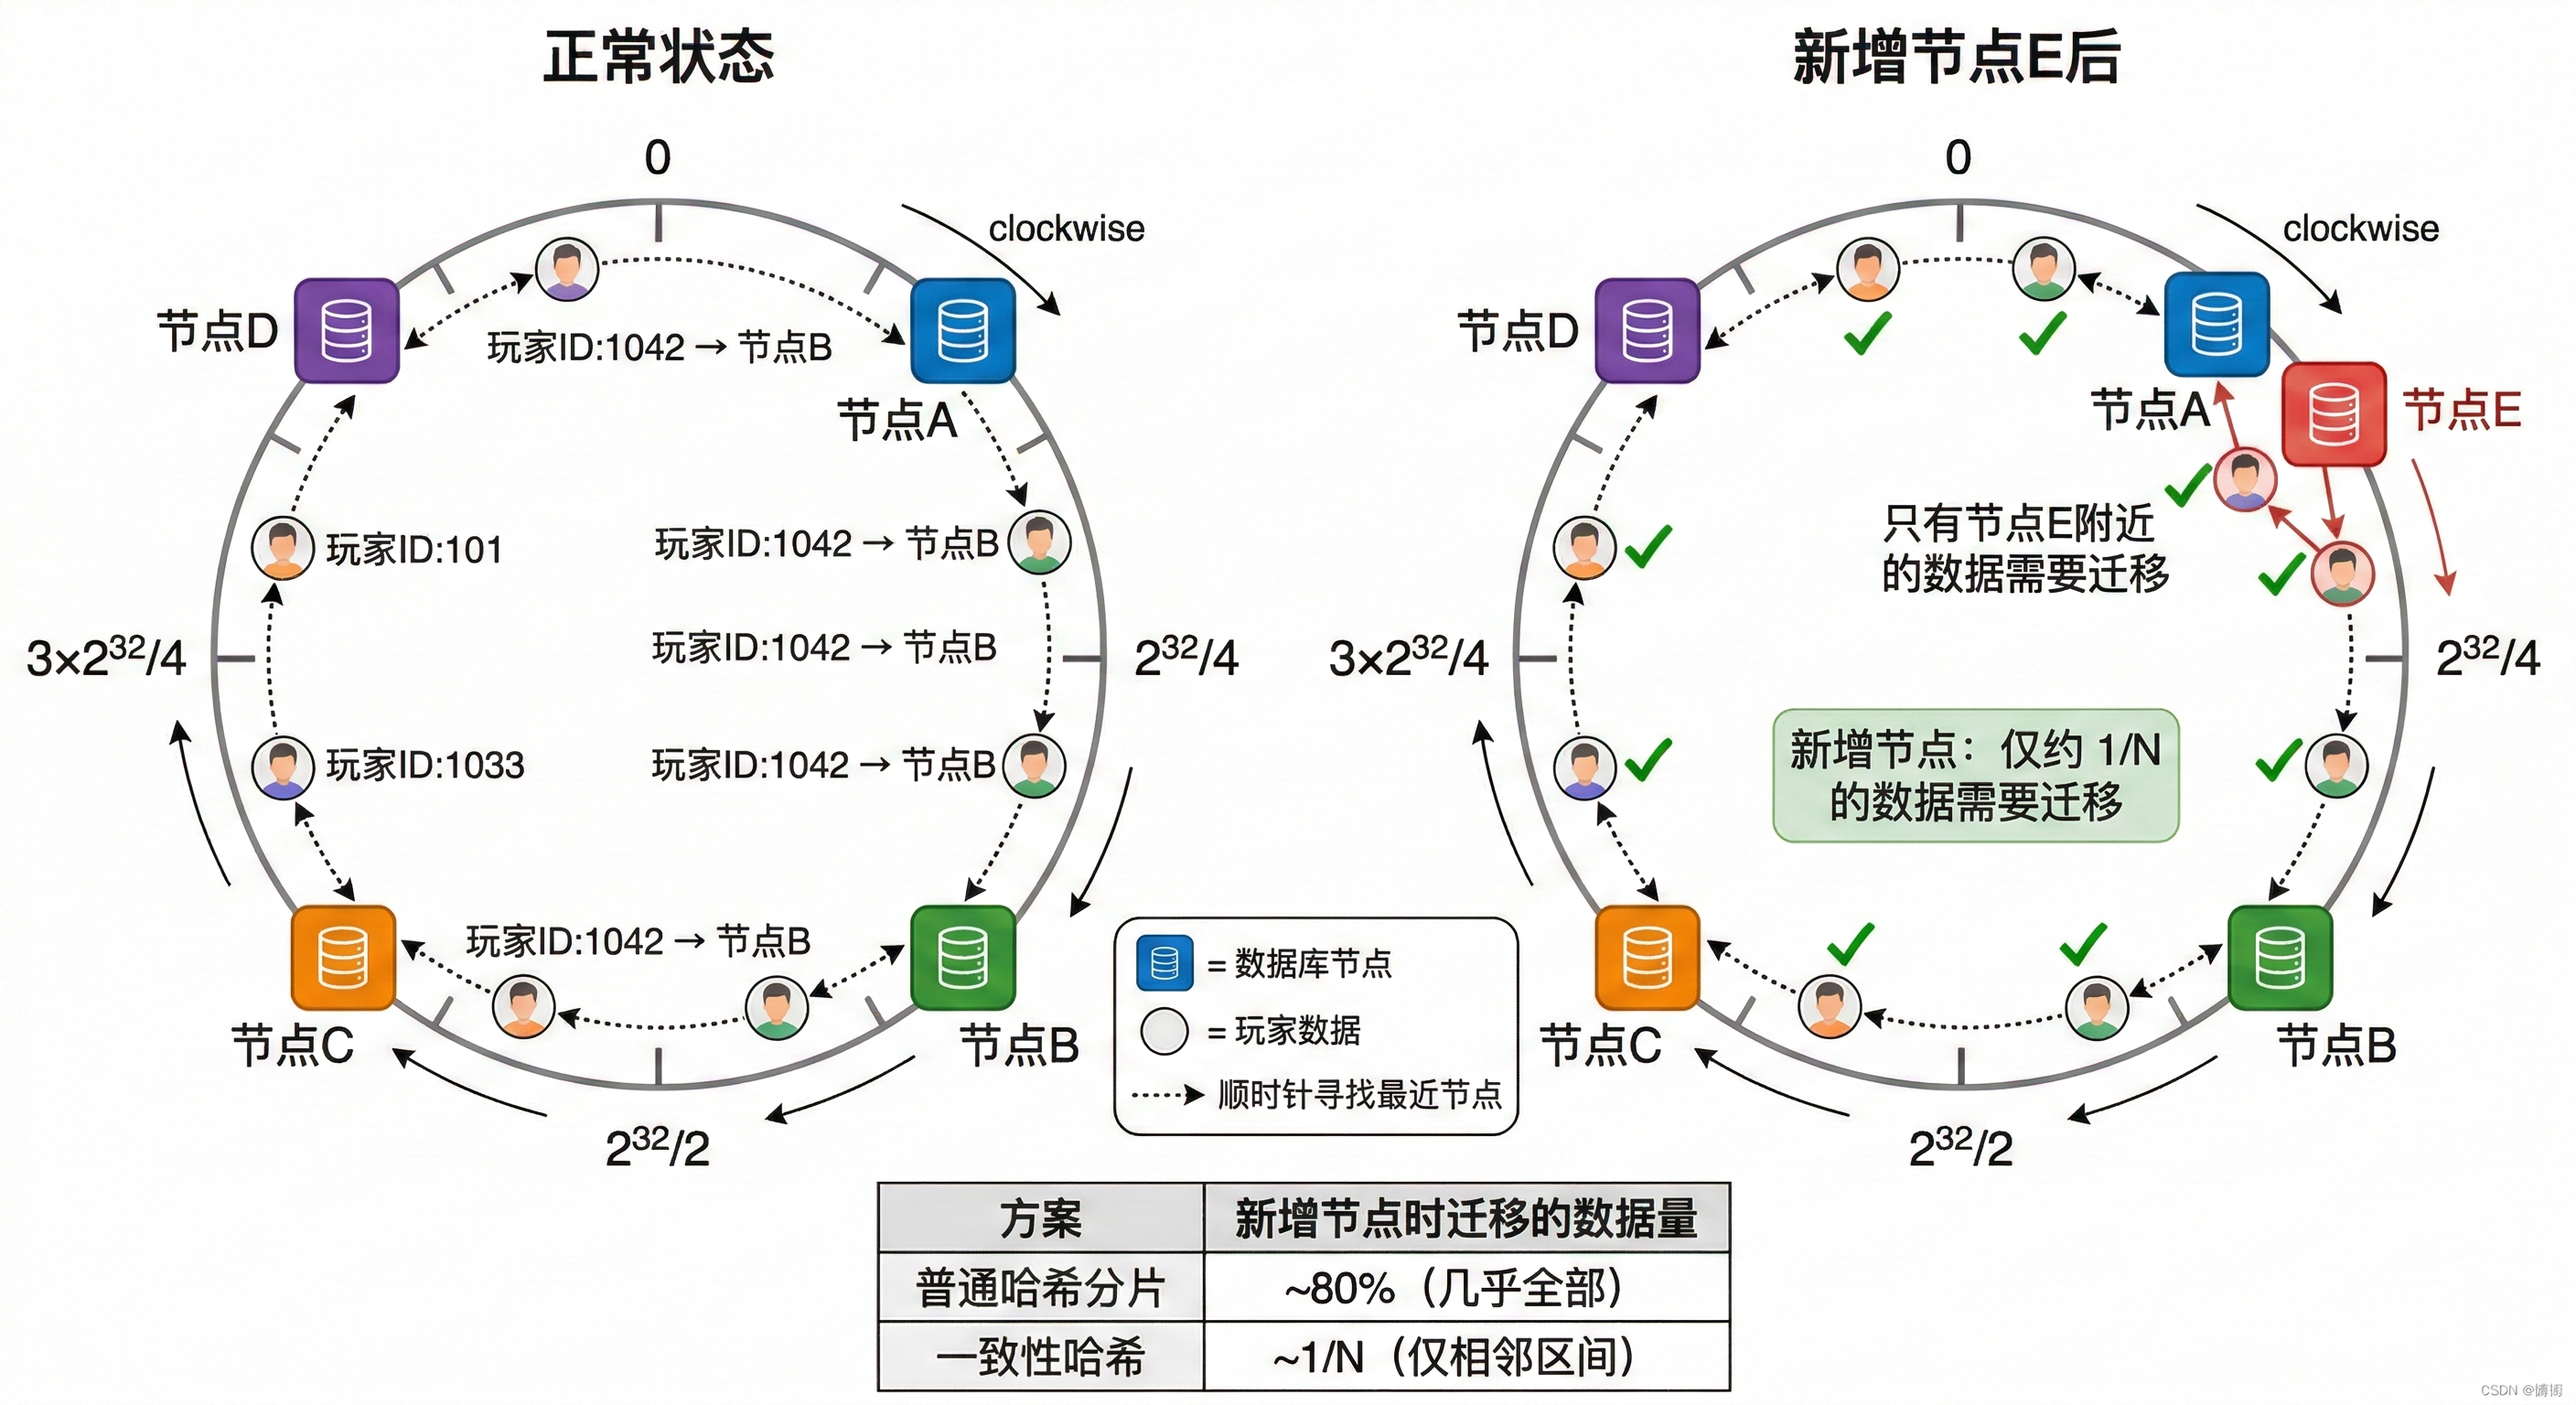
\includegraphics[width=1\linewidth]{figures/sec4/4-6.png}
    \caption{一致性哈希环示意：数据库节点与玩家ID均映射到哈希环上，玩家数据存储在顺时针方向最近的节点；新增节点时，只有该节点附近区间的数据需要迁移，大幅降低扩容成本}
    \label{fig:consistent_hashing}
\end{figure}

\subsubsection{一致性哈希的算法描述}

一致性哈希算法由三个核心操作组成：构建哈希环、路由查询和节点变更。哈希环本质上是一个有序的键值映射结构，其中键是哈希值（整数），值是对应的数据库节点标识。初始化时，对每个数据库节点的标识（如节点名称或 IP 地址）应用哈希函数，将得到的哈希值作为该节点在环上的位置。为了保证负载均衡，通常还会引入虚拟节点：每个物理节点对应环上的多个位置，每个位置通过对节点标识加上不同的后缀再次哈希得到。哈希环使用有序列表维护所有虚拟节点的位置，这是为了在查询时能够使用二分查找，将路由的时间复杂度控制在 $O(\log n)$，其中 $n$ 是虚拟节点的总数。虚拟节点的键由"节点名\#副本编号"拼接后哈希得到，确保同一物理节点的多个虚拟节点在环上的分布尽量分散，从而让不同物理节点负责的数据区间趋于均匀。

\begin{tcolorbox}[title=算法一：构建一致性哈希环]
\begin{lstlisting}[style=codeblock, language=go]
type HashRing struct {
    ring     map[uint32]string
    sorted   []uint32
    replicas int
}

func BuildRing(nodes []string, replicas int) *HashRing {
    r := &HashRing{
        ring:     make(map[uint32]string),
        replicas: replicas,
    }
    for _, node := range nodes {
        AddNode(r, node)
    }
    return r
}

func AddNode(r *HashRing, node string) {
    for i := 0; i < r.replicas; i++ {
        key := hash(fmt.Sprintf("%s#%d", node, i))
        r.ring[key] = node
        r.sorted = append(r.sorted, key)
    }
    sort.Slice(r.sorted, func(i, j int) bool {
        return r.sorted[i] < r.sorted[j]
    })
}
\end{lstlisting}
\end{tcolorbox}

给定一个玩家 ID，查询其应存放的数据库节点时，算法首先对玩家 ID 求哈希，得到其在环上的位置，然后在有序的虚拟节点列表中找到第一个大于等于该位置的节点，即为顺时针方向最近的节点。若玩家的哈希值大于环上所有节点的位置（即已经超过了最大刻度），则顺时针绕回环的起点，取第一个节点。路由查询的正确性依赖于"顺时针最近"的语义——对于任意玩家 ID，其归属节点唯一确定，不存在歧义。这也保证了在节点集合不变的情况下，同一个玩家 ID 每次查询都会路由到同一个节点，满足缓存和分片场景下的稳定性要求。

\begin{tcolorbox}[title=算法二：路由查询]
\begin{lstlisting}[style=codeblock, language=go]
func Lookup(r *HashRing, playerID string) string {
    if len(r.ring) == 0 {
        return ""
    }
    h := hash(playerID)
    idx := sort.Search(len(r.sorted), func(i int) bool {
        return r.sorted[i] >= h
    })
    if idx == len(r.sorted) {
        idx = 0
    }
    return r.ring[r.sorted[idx]]
}
\end{lstlisting}
\end{tcolorbox}

一致性哈希的核心优势体现在节点变更时的迁移范围。当新增一个物理节点时，该节点的若干虚拟节点被插入哈希环。对于每一个新插入的虚拟节点 $v_{new}$，设其在环上的位置为 $p_{new}$，其顺时针方向的下一个节点为 $v_{next}$，位置为 $p_{next}$。那么，只有原本落在区间 $(p_{prev},\, p_{new}]$ 内的玩家数据需要从 $v_{next}$ 迁移到 $v_{new}$，其中 $p_{prev}$ 是 $v_{new}$ 逆时针方向的前一个节点位置，环上其余区间的数据归属完全不受影响。整体迁移量约占全部数据的 $\frac{1}{N+1}$，其中 $N$ 为原有物理节点数。当 $N = 4$ 时，新增第 5 个节点仅需迁移约 $20\%$ 的数据，而普通哈希分片在同等情况下需要迁移约 $80\%$，体现出一致性哈希在水平扩展场景下的显著优势。

\begin{tcolorbox}[title=算法三：新增节点时计算需要迁移的数据范围]
\begin{lstlisting}[style=codeblock, language=go]
type MigrateRange struct {
    From     string
    To       string
    StartKey uint32
    EndKey   uint32
}

func MigrateRanges(r *HashRing, newNode string) []MigrateRange {
    var ranges []MigrateRange
    for i := 0; i < r.replicas; i++ {
        newKey := hash(fmt.Sprintf("%s#%d", newNode, i))
        idx := sort.SearchUints(r.sorted, newKey)
        var prevKey uint32
        if idx == 0 {
            prevKey = r.sorted[len(r.sorted)-1]
        } else {
            prevKey = r.sorted[idx-1]
        }
        srcNode := r.ring[r.sorted[idx%len(r.sorted)]]
        ranges = append(ranges, MigrateRange{
            From:     srcNode,
            To:       newNode,
            StartKey: prevKey,
            EndKey:   newKey,
        })
    }
    return ranges
}
\end{lstlisting}
\end{tcolorbox}

从算法三可以清楚地看到，需要迁移的数据区间数量等于虚拟节点数 \texttt{replicas}，而每个区间的大小约为 $\frac{1}{N+1}$ 的环空间。这种局部迁移的特性，使得系统能够更加平滑地进行水平扩展，减少了扩容对线上服务的影响。

一致性哈希的优势在于扩容时的迁移成本大大降低。当我们新增一个数据库实例时，只有环上部分位置的数据需要迁移——具体来说，只有新实例与其顺时针方向下一个实例之间的那一段数据需要重新分配，其他数据则保持不变。假设原本有 4 个分片均匀分布在环上，每个分片负责 25\% 的数据；当我们新增第 5 个分片时，只有约 20\% 的数据需要迁移，其余 80\% 的数据不受影响。

在实际应用中，为了进一步提升负载均衡的效果，通常会引入虚拟节点的概念。每个物理数据库实例在哈希环上不是只占据一个位置，而是对应多个虚拟节点（比如 150 个），这些虚拟节点均匀分布在环上。这样做的好处是即使物理节点数量较少，也能通过虚拟节点实现更均匀的数据分布，避免因哈希函数的随机性导致某些物理节点负载过高。虚拟节点数 \texttt{replicas} 的选择需要在负载均衡精度和内存开销之间取得平衡：虚拟节点数越多，各物理节点在环上的分布越均匀，负载偏差越小，但同时哈希环占用的内存也线性增长，查询时的二分查找开销也略有上升。在实际工程中，每个物理节点配置 100 到 200 个虚拟节点是常见的经验值，此时各节点的负载标准差通常可以控制在 5\% 以内，足以满足生产环境的均衡要求。对于我们的游戏服务器场景，若有 4 个数据库分片，配置 150 个虚拟节点意味着哈希环上共有 600 个条目，内存开销极小，但负载分布已经足够均匀，是工程性价比较高的选择。

\subsubsection{分片路由的实现}

理解了分片策略之后，接下来需要解决的问题是：应用层如何知道某个玩家的数据在哪个分片上？这就需要实现一个分片路由层。分片路由层维护着分片规则和分片实例信息，负责将应用层的数据库请求转发到正确的分片上。

最直接的实现方式是在应用层代码中嵌入分片路由逻辑。应用服务器启动时，从配置文件或配置中心读取分片规则（比如使用哈希分片，共 4 个分片）和各分片的数据库连接信息（IP 地址、端口、账号密码等），构建一个分片路由表。当需要查询某个玩家的数据时，应用层先根据玩家 ID 和分片规则计算出目标分片编号，再从路由表中获取对应的数据库连接，最后向该数据库发起查询。

\begin{tcolorbox}[title=应用层分片路由的实现示例]
\begin{lstlisting}[
    language=go,
    basicstyle=\ttfamily\footnotesize,
    aboveskip=0pt, belowskip=0pt,
    lineskip=-1pt,
    commentstyle=\color{gray},
    keywordstyle=\color{blue}\bfseries,
    breaklines=true
]
// 分片路由器
type ShardRouter struct {
    numShards int
    dbConnections []*sql.DB  // 各分片的数据库连接
}

// 根据玩家ID获取目标分片的数据库连接
func (r *ShardRouter) getDBConnection(playerID int) *sql.DB {
    shardID := playerID % r.numShards
    return r.dbConnections[shardID]
}

// 查询玩家数据
func (r *ShardRouter) queryPlayer(playerID int) (*Player, error) {
    // 1. 计算目标分片
    db := r.getDBConnection(playerID)
    
    // 2. 向目标分片发起查询
    var player Player
    err := db.QueryRow(
        "SELECT id, name, power FROM players WHERE id = ?",
        playerID,
    ).Scan(&player.ID, &player.Name, &player.Power)
    
    return &player, err
}
\end{lstlisting}
\end{tcolorbox}

这种应用层路由的优点是实现简单、性能开销低——路由计算只是一个简单的取模操作，几乎不消耗时间。但缺点也很明显：分片逻辑与业务代码耦合在一起，如果需要调整分片策略（比如从哈希分片改为一致性哈希）或增加分片数量，可能需要修改应用层代码并重新部署。

另一种实现方式是引入数据库代理中间件（Database Proxy）。中间件作为独立的服务部署在应用服务器和数据库之间，应用层不再直接连接各个分片，而是统一连接到中间件。中间件负责接收应用层的 SQL 请求，解析 SQL 语句，提取分片键（如 WHERE 子句中的玩家 ID），计算目标分片，将请求转发到对应的数据库实例，最后将结果返回给应用层。这种方式的优点是业务代码与分片逻辑完全解耦，分片策略的调整不需要修改应用代码；缺点是引入了额外的网络跳转和 SQL 解析开销，可能对性能有一定影响。

\subsubsection{分片后的查询与事务挑战}

数据拆分完成之后，应用层所面对的数据库世界已经发生了根本性的变化。这种变化不仅体现在连接方式和路由逻辑上，更深刻地影响了某些类型查询和事务的实现方式。

首先是跨分片查询的问题。前面提到的分片路由，针对的是"查询单个玩家数据"这种场景——给定一个玩家 ID，我们可以明确地知道数据在哪个分片，直接向该分片发起查询即可。但有些查询并不是针对单个玩家的，而是需要聚合多个分片的数据。最典型的例子是全服排行榜：假设我们需要查询战力值排名前一百的玩家。

在单一数据库时代，这只需要执行一条 SQL 语句：

\begin{tcolorbox}[title=单一数据库中的排行榜查询]
\begin{lstlisting}[
    language=SQL,
    basicstyle=\ttfamily\footnotesize,
    aboveskip=0pt, belowskip=0pt,
    lineskip=-1pt,
    commentstyle=\color{gray},
    keywordstyle=\color{blue}\bfseries,
    breaklines=true
]
SELECT id, name, power 
FROM players 
ORDER BY power DESC 
LIMIT 100;
-- 数据库自动扫描所有玩家，按战力排序，返回前100名
\end{lstlisting}
\end{tcolorbox}

但在数据拆分之后，不同玩家的数据分散在不同的分片中。应用层需要采用"分散查询、集中汇总"的策略：首先向所有分片分别发起查询，每个分片返回自己负责的那部分玩家中战力值最高的 100 个；然后应用层将这些结果合并到一起（比如分片 0 返回 100 个，分片 1 返回 100 个，分片 2 返回 100 个，分片 3 返回 100 个，总共 400 个），在应用层重新排序，最终截取战力值最高的 100 个作为全服排行榜。

\begin{tcolorbox}[title=分片环境下的排行榜查询]
\begin{lstlisting}[
    language=go,
    basicstyle=\ttfamily\footnotesize,
    aboveskip=0pt, belowskip=0pt,
    lineskip=-1pt,
    commentstyle=\color{gray},
    keywordstyle=\color{blue}\bfseries,
    breaklines=true
]
func (r *ShardRouter) getRanking() ([]Player, error) {
    var allResults []Player
    
    // 1. 向所有分片并发发起查询
    for i := 0; i < r.numShards; i++ {
        var shardResults []Player
        rows, _ := r.dbConnections[i].Query(
            "SELECT id, name, power FROM players ORDER BY power DESC LIMIT 100",
        )
        // 读取该分片的Top100到shardResults...
        allResults = append(allResults, shardResults...)
    }
    
    // 2. 在应用层合并并重新排序
    sort.Slice(allResults, func(i, j int) bool {
        return allResults[i].Power > allResults[j].Power
    })
    
    // 3. 截取最终的Top100
    if len(allResults) > 100 {
        allResults = allResults[:100]
    }
    
    return allResults, nil
}
\end{lstlisting}
\end{tcolorbox}

这种跨分片查询的效率明显低于单库查询。首先，需要向多个分片发起查询，网络开销成倍增加；其次，每个分片都要执行完整的排序操作，计算资源消耗是单库的数倍；最后，应用层还需要对合并后的结果进行二次排序，增加了应用服务器的 CPU 负担。因此，在设计分片策略时，应尽量避免频繁的跨分片查询。对于排行榜这类必须进行全局聚合的数据，更好的做法是采用异步汇总：通过后台定时任务，定期从各个分片拉取数据并汇总到一个专门的"排行榜缓存"中（比如 Redis），玩家查询排行榜时直接读取缓存，而不是实时跨分片查询。

更棘手的是跨分片事务问题。在我们的对战游戏中，假设玩家 A（ID 为 1001，存储在分片 1）与玩家 B（ID 为 2002，存储在分片 2）进行了一场战斗。战斗结束后，需要同时更新两位玩家的战绩：

\begin{enumerate}
\item 在分片 1 中更新玩家 A 的胜场数：\texttt{UPDATE players SET wins = wins + 1 WHERE id = 1001}
\item 在分片 2 中更新玩家 B 的负场数：\texttt{UPDATE players SET losses = losses + 1 WHERE id = 2002}
\end{enumerate}

在单一数据库中，这两个操作可以放在同一个事务中，数据库保证要么全部成功
（玩家 A 的胜场加一，玩家 B 的败场加一），要么全部失败（都回滚，谁的战绩都不变）。
但在拆分后的世界里，这两个操作分别发生在两个独立的数据库实例上。
如果简单地依次执行，就可能出现"部分成功"的情况：
第一个操作成功了（A 的胜场已经加一），第二个操作却因为网络故障失败了（B 的败场没有更新），
数据库里就留下了一场只有赢家、没有输家的战斗记录——这正是分布式环境下事务一致性问题的典型表现。

要解决跨分片事务问题，需要引入分布式事务协议，最经典的是两阶段提交协议
（Two-Phase Commit，2PC）。其完整流程如图~\ref{fig:2pc} 所示。
第一阶段称为准备阶段（Prepare Phase）：由一个协调者（Coordinator）同时向所有参与事务的分片
发出"准备提交"请求（图中步骤①）。各分片收到请求后，在本地执行操作并将结果写入事务日志，
但不立即提交，而是对相关数据行加锁以防止其他事务并发修改，然后向协调者回复"就绪"
（Vote: Ready）或"失败"（Vote: Abort）（图中步骤②）。
这把锁不会在准备阶段结束——它必须一直持续到协调者发出第二阶段的最终指令为止，
图中红色括注的区间正是行锁被持有的全程，这也是 2PC 拉长锁持有时间、降低并发度的根本原因。

第二阶段称为提交阶段（Commit Phase）：协调者收集完所有分片的投票后进行裁决（图中步骤③）。
若所有分片均回复"就绪"，协调者向所有分片广播"正式提交"指令，
各分片将准备好的操作真正落库并释放行锁（图中成功路径步骤④）；
若任意一个分片回复"失败"，或协调者在超时时间内未收到全部响应，
则广播"回滚"指令，各分片撤销准备阶段的操作并同样释放锁（图中失败路径步骤④）。
在我们的战斗场景中，这意味着玩家 A 的胜场更新和玩家 B 的败场更新要么同时落库，
要么同时撤销，从协议层面保证了跨分片操作的原子性。

然而 2PC 的代价是显著的，体现在图中三个灰色注记上。
其一，整个流程涉及两轮网络往返——准备阶段一轮，提交阶段一轮——
每轮都需要协调者与全部参与分片完成请求和响应，事务的端到端延迟远高于单分片事务。
其二，准备阶段到提交阶段之间行锁持续持有，其他需要读写同一数据行的事务都要排队等待，
在高并发的游戏场景下这会显著压缩系统的吞吐量上限。
其三，协调者存在单点崩溃风险：若协调者在广播"准备"之后、发出"提交"之前宕机，
各分片将永远停留在"就绪"状态，行锁无法自动释放，后续所有操作都会被阻塞，
必须依靠超时机制或人工介入才能恢复，这在生产环境中是极难排查的故障场景。

\begin{figure}[htbp]
    \centering
    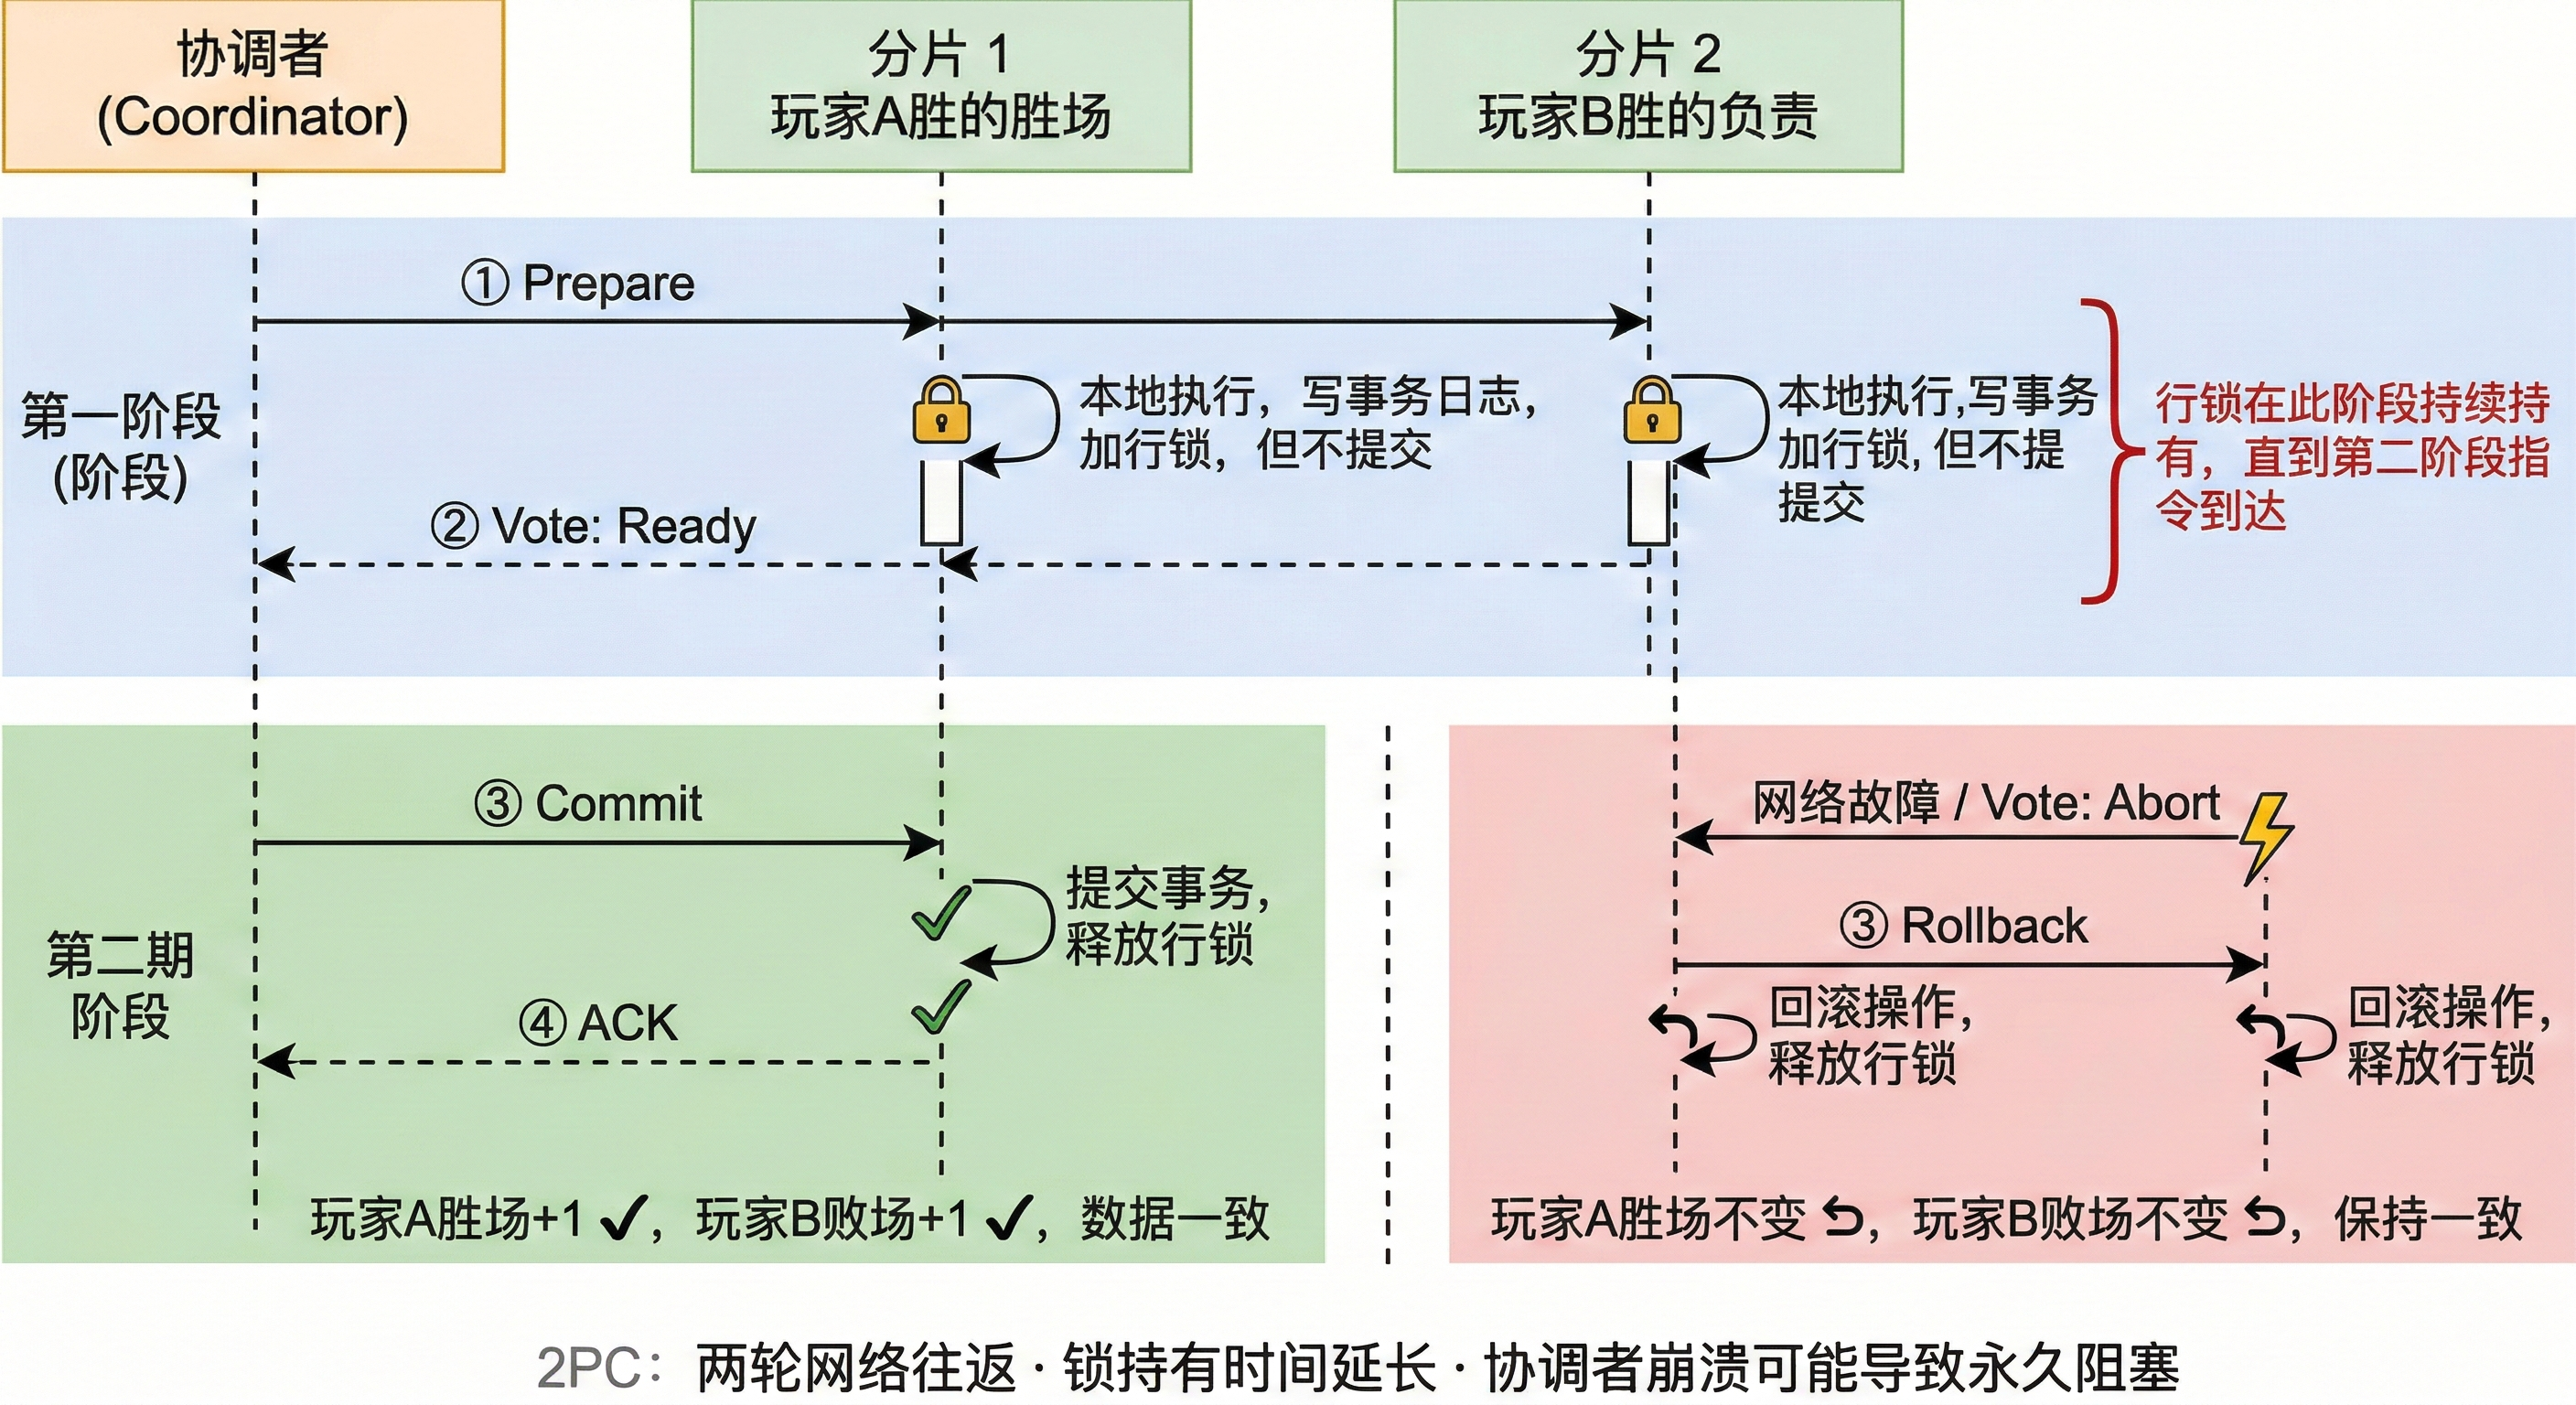
\includegraphics[width=1\linewidth]{figures/sec4/两阶段提交.png}
    \caption{两阶段提交协议（2PC）的时序图：第一阶段协调者收集各分片的投票并持锁等待，
    第二阶段根据投票结果广播提交或回滚指令；红色括注区间为行锁持有期，
    右侧失败路径展示协调者收到 Abort 或超时后触发全局回滚的流程}
    \label{fig:2pc}
\end{figure}

因此，在实际工程中引入 2PC 的代价往往超过其带来的收益。
更实用的做法是从业务设计层面入手，将跨分片操作转化为可以在单分片内完成的操作，
或者接受短暂的数据不一致并通过异步机制保证最终收敛。
这里介绍两种常见的工程策略。

第一种策略是异步消息队列。战斗结束后，战斗服务器不直接向两个分片发起写操作，
而是将战斗结果——包括双方玩家 ID、胜负情况、时间戳——作为一条消息投递到消息队列。
专门的战绩更新服务从队列中消费消息，依次向各分片发起更新；
若某次更新因分片暂时不可用而失败，消息会保留在队列中持续重试，最终一定会被成功处理，
不存在"永久丢失"的风险。这种方案以"最终一致性"替代"强一致性"——
战绩会在数秒内更新完毕，对玩家几乎无感知，系统换来的是更高的可用性和远低于 2PC 的实现复杂度。
需要注意的是，消息队列本身必须具备持久化和至少一次投递的保障，
否则队列自身的故障反而会成为新的数据丢失入口。

第二种策略是重新设计数据模型，从根本上消除跨分片事务存在的前提。
如果战绩是高频写入的核心数据，可以将战绩从玩家分片中完全剥离，
交由一个独立的战绩服务集中管理。这个服务可以使用单一数据库（若数据量可控），
也可以使用专门为追加写入优化的时序数据库，所有对战绩的读写操作都发生在该服务内部，
从结构上不再存在跨分片写入的问题。代价是系统多了一个独立服务和对应的数据库，
运维复杂度略有上升；但换来的是战绩访问路径的简单清晰——
尤其对于玩家查询历史对战记录这类高频只读场景，单服务内的查询比跨分片聚合要高效得多。


\subsubsection{容错机制与备份策略}

数据拆分到多个数据库实例之后，虽然降低了单点故障的全局影响，但每个数据库实例仍然需要有自己的容错机制。最常见的做法是为每个数据库实例部署主从复制架构（Master-Slave Replication）。

在主从架构中，每个分片包含一个主库（Master）和一个或多个从库（Slave）。主库负责处理所有的写操作（INSERT、UPDATE、DELETE），从库通过 binlog（二进制日志）实时同步主库的数据变化，并承担读操作的负载。具体的同步过程是：主库在执行每个写操作时，会将操作记录到 binlog 中；从库会持续监听主库的 binlog，读取新的日志条目，并在本地重放（Replay）这些操作，从而保持与主库的数据一致。

\begin{figure}[htbp]
    \centering
    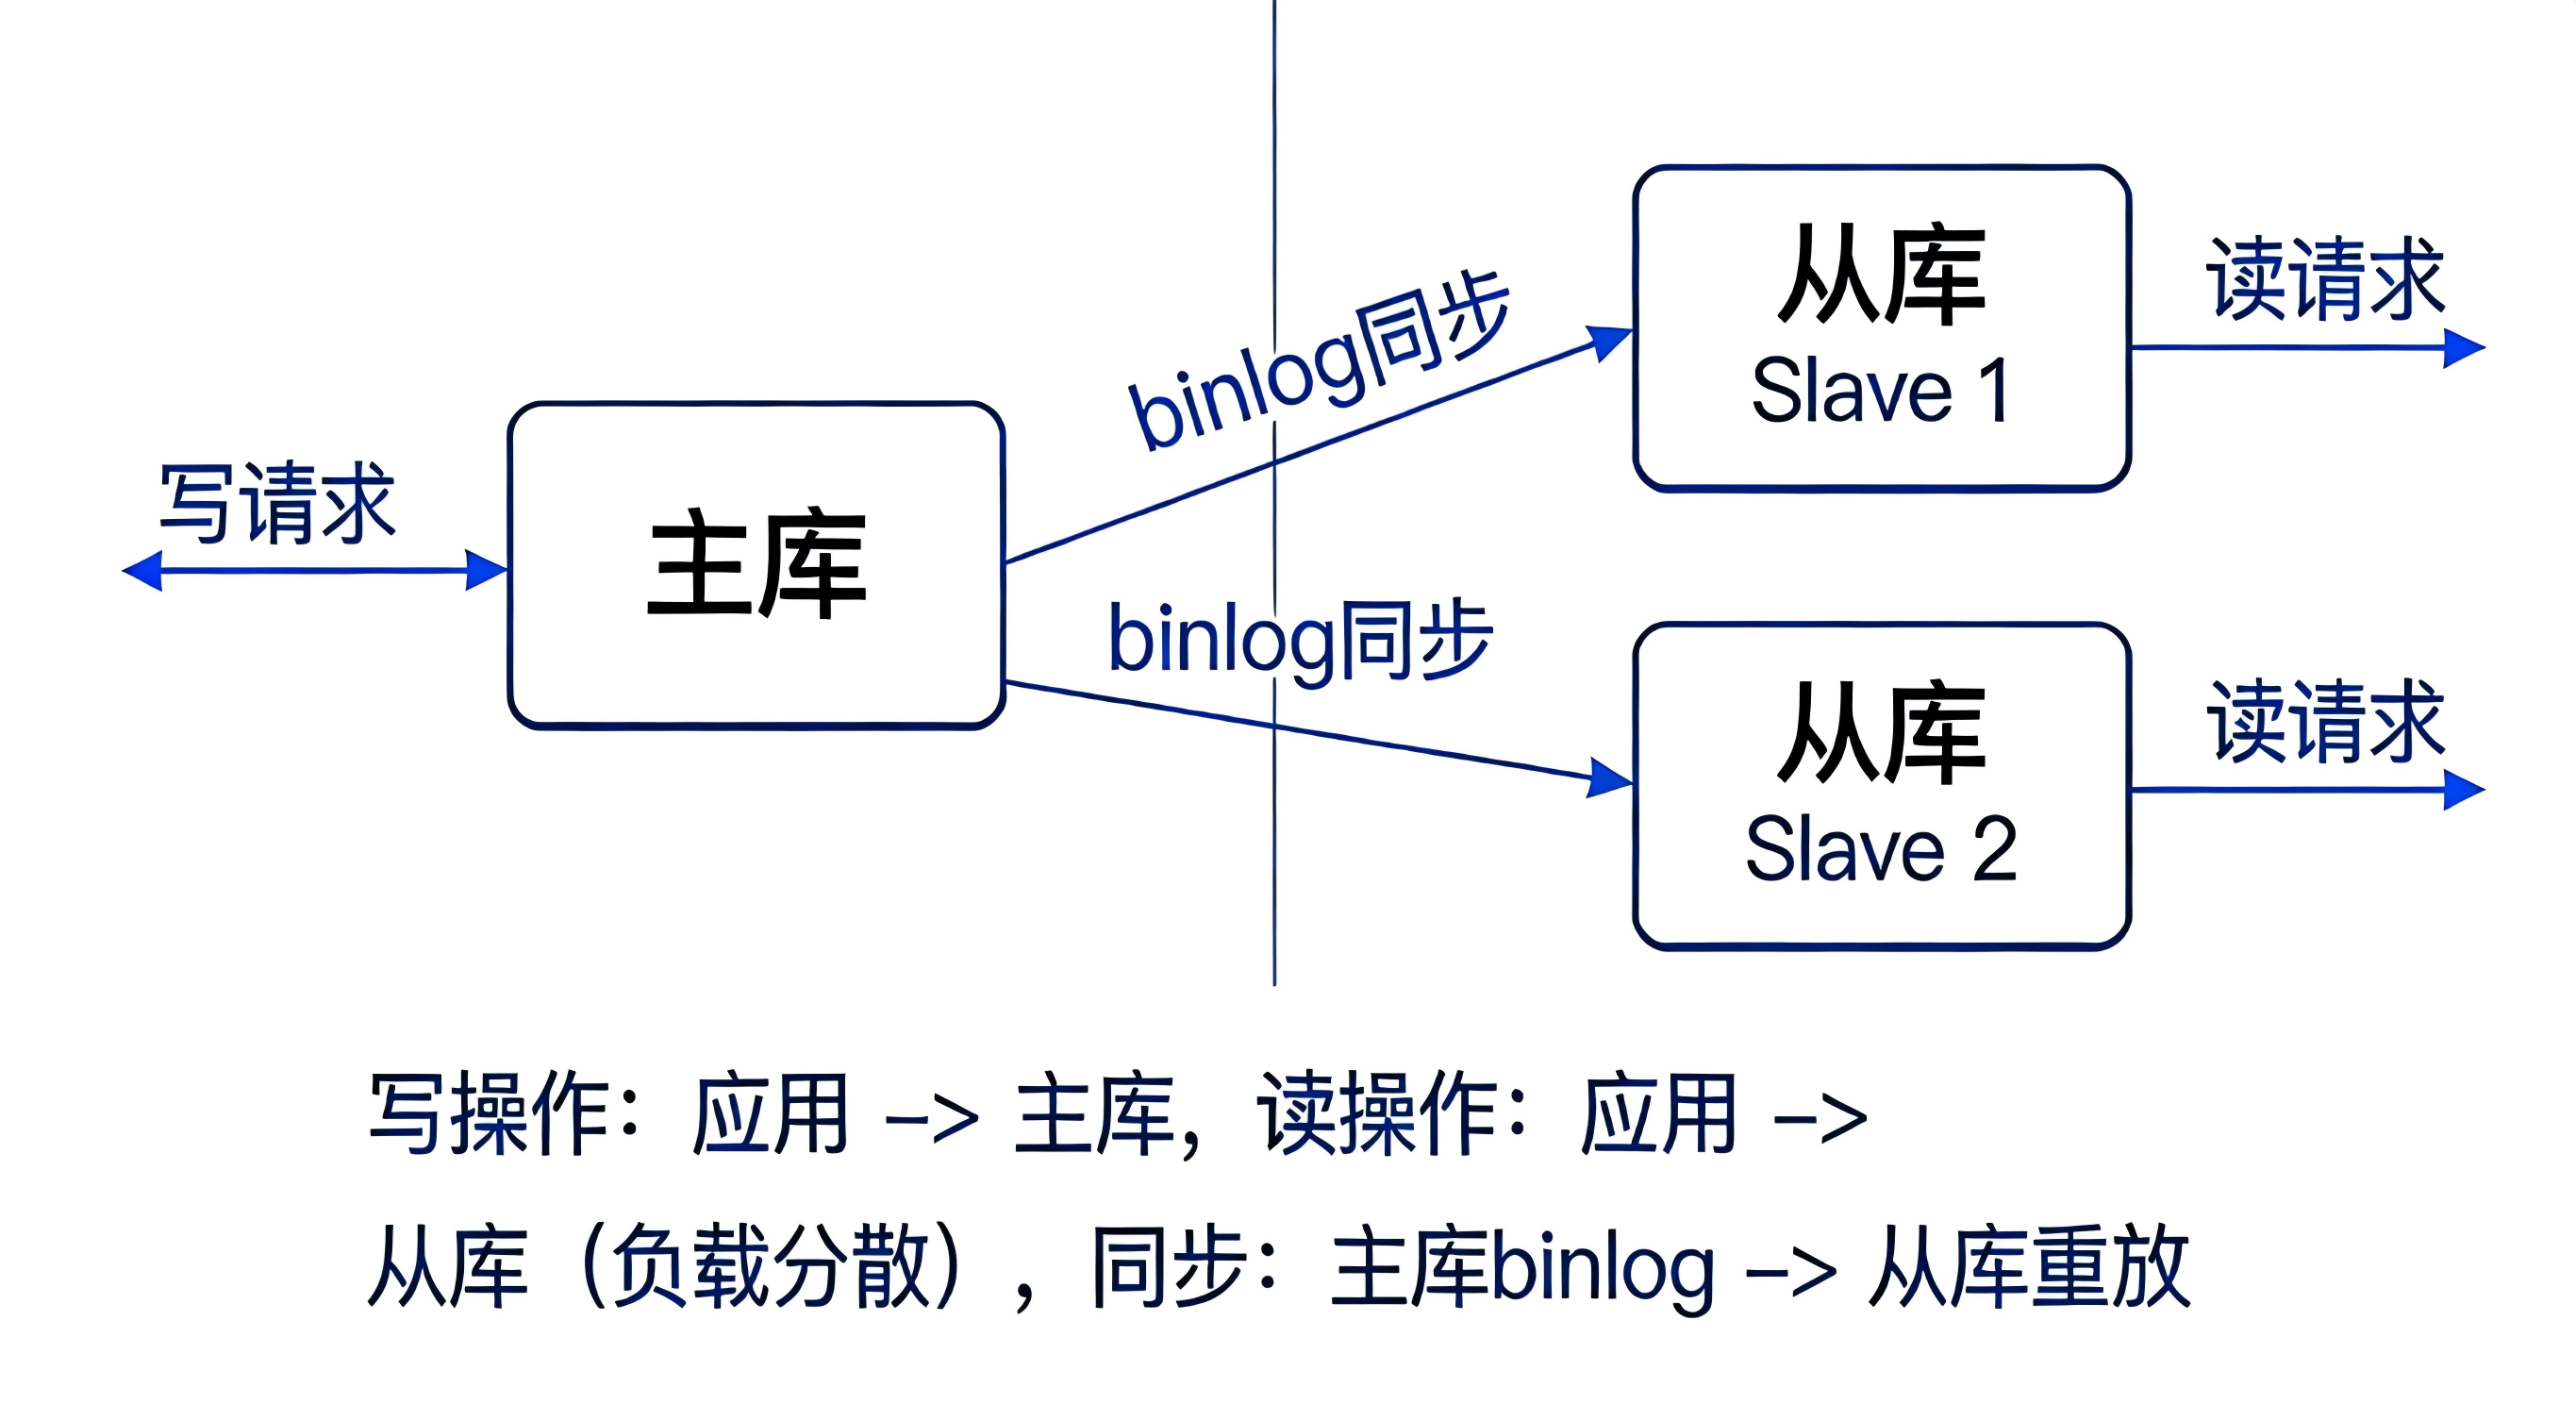
\includegraphics[width=1\linewidth]{figures/sec4/4-3.png}
    % 图片描述：主从复制架构示意图
    % 左侧：一个"主库"矩形框，标注"Master"，接收"写请求"箭头
    % 右侧：两个"从库"矩形框，标注"Slave 1"和"Slave 2"，接收"读请求"箭头
    % 主库向两个从库各有一条箭头，标注"binlog同步"
    % 下方用文字说明：
    %   - 写操作：应用 -> 主库
    %   - 读操作：应用 -> 从库（负载分散）
    %   - 同步：主库binlog -> 从库重放
    % 所有文字使用简体中文
    \caption{数据库主从复制架构}
    \label{fig:master_slave_replication}
\end{figure}

这种主从架构有两个核心好处。第一，提升了读取并发能力。由于大部分游戏场景中读操作远多于写操作（比如玩家登录时读取角色信息、查看背包、查询战绩等），将读请求分散到多个从库上，可以有效降低主库的压力，提升系统的整体查询吞吐量。应用层可以采用简单的轮询策略，将读请求依次分配给不同的从库，或者根据从库的负载情况动态选择。

第二，实现了数据的热备份。当主库出现故障时——比如硬件损坏、进程崩溃、网络中断——可以快速将某个从库提升为新的主库（这个过程称为故障转移，Failover），继续提供服务。具体的故障转移流程通常由自动化工具或数据库代理中间件来完成：首先，通过心跳检测发现主库不可用；然后，从多个从库中选择一个数据最新、延迟最低的作为新主库；接着，通知应用层和其他从库切换连接目标；最后，新主库开始接收写请求，其他从库从新主库同步数据。整个过程通常可以在数十秒内完成，大大缩短了故障恢复时间。

除了主从复制，还需要建立完善的备份策略。主从复制虽然提供了实时的热备份，但它无法防范某些类型的错误——比如误操作删除了大量数据，或者数据被恶意篡改。这种情况下，从库会同步主库的错误操作，热备份无法起到保护作用。因此，我们还需要定期执行冷备份：

全量备份（Full Backup）：定期（比如每天凌晨）对整个数据库做一次完整的快照，导出所有表的数据和结构，存储到独立的备份服务器或云存储服务（如 Amazon S3、阿里云 OSS）中。全量备份的好处是恢复简单——只需要将备份文件导入即可恢复到备份时刻的完整状态；缺点是备份文件较大，占用存储空间多，备份和恢复过程耗时较长。

增量备份（Incremental Backup）：在两次全量备份之间，定期（比如每小时）备份自上次备份以来发生变化的数据。增量备份通常通过备份 binlog 来实现——binlog 记录了所有的数据变更操作，通过重放 binlog 可以将数据库恢复到任意时间点。增量备份的好处是备份文件小、备份速度快；缺点是恢复时需要先恢复最近的全量备份，再依次重放所有增量备份，过程较复杂。

在实际部署中，通常会结合全量备份和增量备份：每天做一次全量备份，每小时做一次增量备份。这样，当需要恢复数据时，可以先恢复最近的全量备份（比如昨天凌晨的），再重放之后的增量备份（昨天凌晨到故障时刻之间的 binlog），将数据恢复到故障发生前的最新状态，数据丢失的时间窗口可以控制在一小时以内。

最后，备份的存在只是保障的第一步，更关键的是要定期进行恢复演练。很多系统在真正需要恢复数据时才发现备份文件损坏、恢复脚本有 bug、或者恢复时间远超预期。因此，建议每月至少进行一次备份恢复演练：在测试环境中，使用真实的备份文件模拟完整的恢复流程，记录恢复所需的时间，发现并修复流程中的问题。通过这些容错机制——主从复制、定期备份、恢复演练——即使某个分片出现故障，也能在最短时间内恢复服务，将对玩家的影响降到最低。



\subsubsection{缓存层的分布式演进：从单机Redis到集群}

% 前面几节讨论了PostgreSQL数据库的分片策略，但不要忘记，在第三章中我们建立的分层存储架构还包含Redis缓存层。当数据库从单实例拆分为多个分片时，Redis同样面临容量和可用性的挑战：单机Redis的内存上限通常在几十GB到上百GB之间，当热数据总量超过这个上限时，单个Redis实例将无法容纳所有在线玩家的实时状态；同时，单机Redis也存在单点故障风险——一旦宕机，所有依赖缓存的热数据访问都会直接穿透到数据库，瞬间压垮后端。

% 解决思路与数据库分片类似：将数据分散到多个Redis节点上。Redis Cluster是官方提供的分布式方案，它将整个键空间划分为16384个哈希槽（Hash Slot），每个节点负责一部分槽位。当应用写入一个键时，Redis客户端通过CRC16哈希算法计算该键应落入哪个槽位，再路由到对应的节点。这种机制与第三章中单机Redis的使用方式在应用层几乎透明——开发者仍然使用相同的SET、GET、ZADD等命令，只是底层的数据分布由集群自动管理。

% 需要注意的是，Redis分片与数据库分片的分片键通常保持一致。如果数据库按玩家ID哈希分片，Redis中以玩家ID为前缀的键（如\texttt{player:1001:pos}、\texttt{player:1001:online}）也应当路由到对应的Redis节点，这样同一个玩家的热数据和冷数据在物理上保持亲和性，避免跨节点访问。对于排行榜这类全局聚合数据，则可以使用独立的Redis实例集中存储，由后台任务定期从各分片汇总更新。

在前文中，我们已经用玩家 ID 作为分片键，将冷数据拆分到多个 PostgreSQL 实例上；从本质上讲，Redis 缓存层面对的是同一类问题：单机内存容量和单点故障风险。当在线玩家规模从几千增长到几十万时，单个 Redis 实例的内存不足以容纳所有玩家的在线状态、实时位置、排行榜片段等热数据，一旦出现故障，所有访问都会瞬间穿透到后端数据库，形成“雪崩效应”。

因此，Redis 层的演进思路与数据库分片是一致的：同样以玩家 ID 作为分片键，将键空间拆分到多个 Redis 节点上，实现容量和吞吐的水平扩展，并通过多节点降低单点故障风险。不同之处在于实现机制：数据库分片可以使用范围分片、哈希分片或一致性哈希，而 Redis 官方的 Redis Cluster 则将整个键空间划分为 16384 个哈希槽（Hash Slot），每个槽位对应一个范围编号，由不同节点负责一部分槽位。

具体来说，当我们在应用中写入一个键时，Redis 客户端会对键名执行 CRC16 哈希运算，再对 16384 取模，得到一个槽位编号；集群根据槽位所属范围，将请求路由到对应节点上。形式上，这与“玩家 ID 经过哈希后落在哈希环上，再映射到某个分片节点”是同一套思路，只是 PostgreSQL 分片由我们自己定义哈希规则，而 Redis Cluster 固定使用“槽位”的抽象。

在具体设计时，有一个需要与数据库分片刻意对齐的点：分片键的一致性。如果数据库是按玩家 ID 进行哈希分片，那么 Redis 中与该玩家相关的缓存键（例如 \texttt{player:1001:pos}、\texttt{player:1001:online}、\texttt{player:1001:inventory}）也应当围绕玩家 ID 组织，并路由到与该玩家冷数据同一个逻辑分片上。对于 Redis Cluster，可以利用哈希标签（Hash Tag）保证相关键落在同一个槽位，例如使用 \texttt{{player:1001}:pos}、\texttt{{player:1001}:online} 的形式，使大括号中的部分作为共同哈希片段，从而将同一玩家的多种状态键聚集在同一节点上，减少跨节点访问和多键操作受限的问题。

% 需要注意的是，Redis 的分片与复制是两条正交的维度：分片解决的是“如何把不同玩家的数据分布到多台节点上”，复制（主从/主备）解决的是“同一份数据如何在多台节点之间做高可用冗余”。在一个成熟的部署中，通常会将前文的思路整体套用到缓存层：每个 Redis 分片节点后面再挂一到多个副本节点，既通过分片实现容量与性能的水平扩展，又通过复制实现故障时的快速切换，避免缓存层成为新的单点短板。

\subsection{负载均衡：合理分配玩家流量}

当数据库和缓存层都完成分布式拆分之后，游戏系统已经具备了在多台机器上存储和管理
玩家数据的能力。但仅有数据层的拆分还不够，计算层——也就是运行游戏逻辑、
处理玩家操作的游戏服务器——同样需要进行扩展和分配。
可以想象这样一个场景：我们把玩家数据分片存储到了四台数据库服务器上，
每台数据库都能稳定地承载 25 万玩家的数据，从存储容量的角度看似乎万事大吉。
但当这 100 万玩家真正上线游戏时，他们需要连接的不是数据库，而是游戏服务器——
游戏服务器负责处理玩家的登录请求、匹配对手、模拟战斗、结算奖励，
这些都是实时的、计算密集的任务。如果我们只部署了一台游戏服务器，
那么即使数据库已经完成了分片，这台游戏服务器仍然会成为新的瓶颈：
它的 CPU 要处理所有玩家的战斗逻辑，它的网络要承载所有玩家的消息收发，
它的内存要维护所有在线玩家的会话状态。

在理解这一问题时，有一个容易产生的误解需要先澄清：游戏服务器与数据库分片之间，
并不存在一一对应的绑定关系。下图展示了这一点。
数据库分片解决的是\textbf{存储层}的问题——将玩家的冷数据按分片键切割，
分散存放到多个独立的数据库实例上，每个分片负责一个哈希区间内的玩家数据。
游戏服务器解决的是\textbf{计算层}的问题——将玩家的实时连接和计算请求分散到多台服务器上，
每台服务器负责维护一部分在线玩家的会话和战斗逻辑。
这两个维度是相互独立的：任意一台游戏服务器在需要读写某个玩家的数据时，
都通过分片路由层计算出目标分片编号，再向对应的数据库实例发起请求——
是"多对多"的访问关系，而不是固定的"服务器 1 专属对应分片 1"的绑定关系。
这种解耦带来了极大的灵活性：当在线玩家数量激增、计算层成为瓶颈时，
我们可以单独增加游戏服务器的数量而无需触动数据库配置；
当玩家数据总量增长、存储层遇到容量上限时，
可以单独为数据库增加新的分片而不必同步扩容游戏服务器。
两个维度按照各自的压力独立伸缩，这正是分层架构的核心价值所在。

\begin{figure}[htbp]
    \centering
    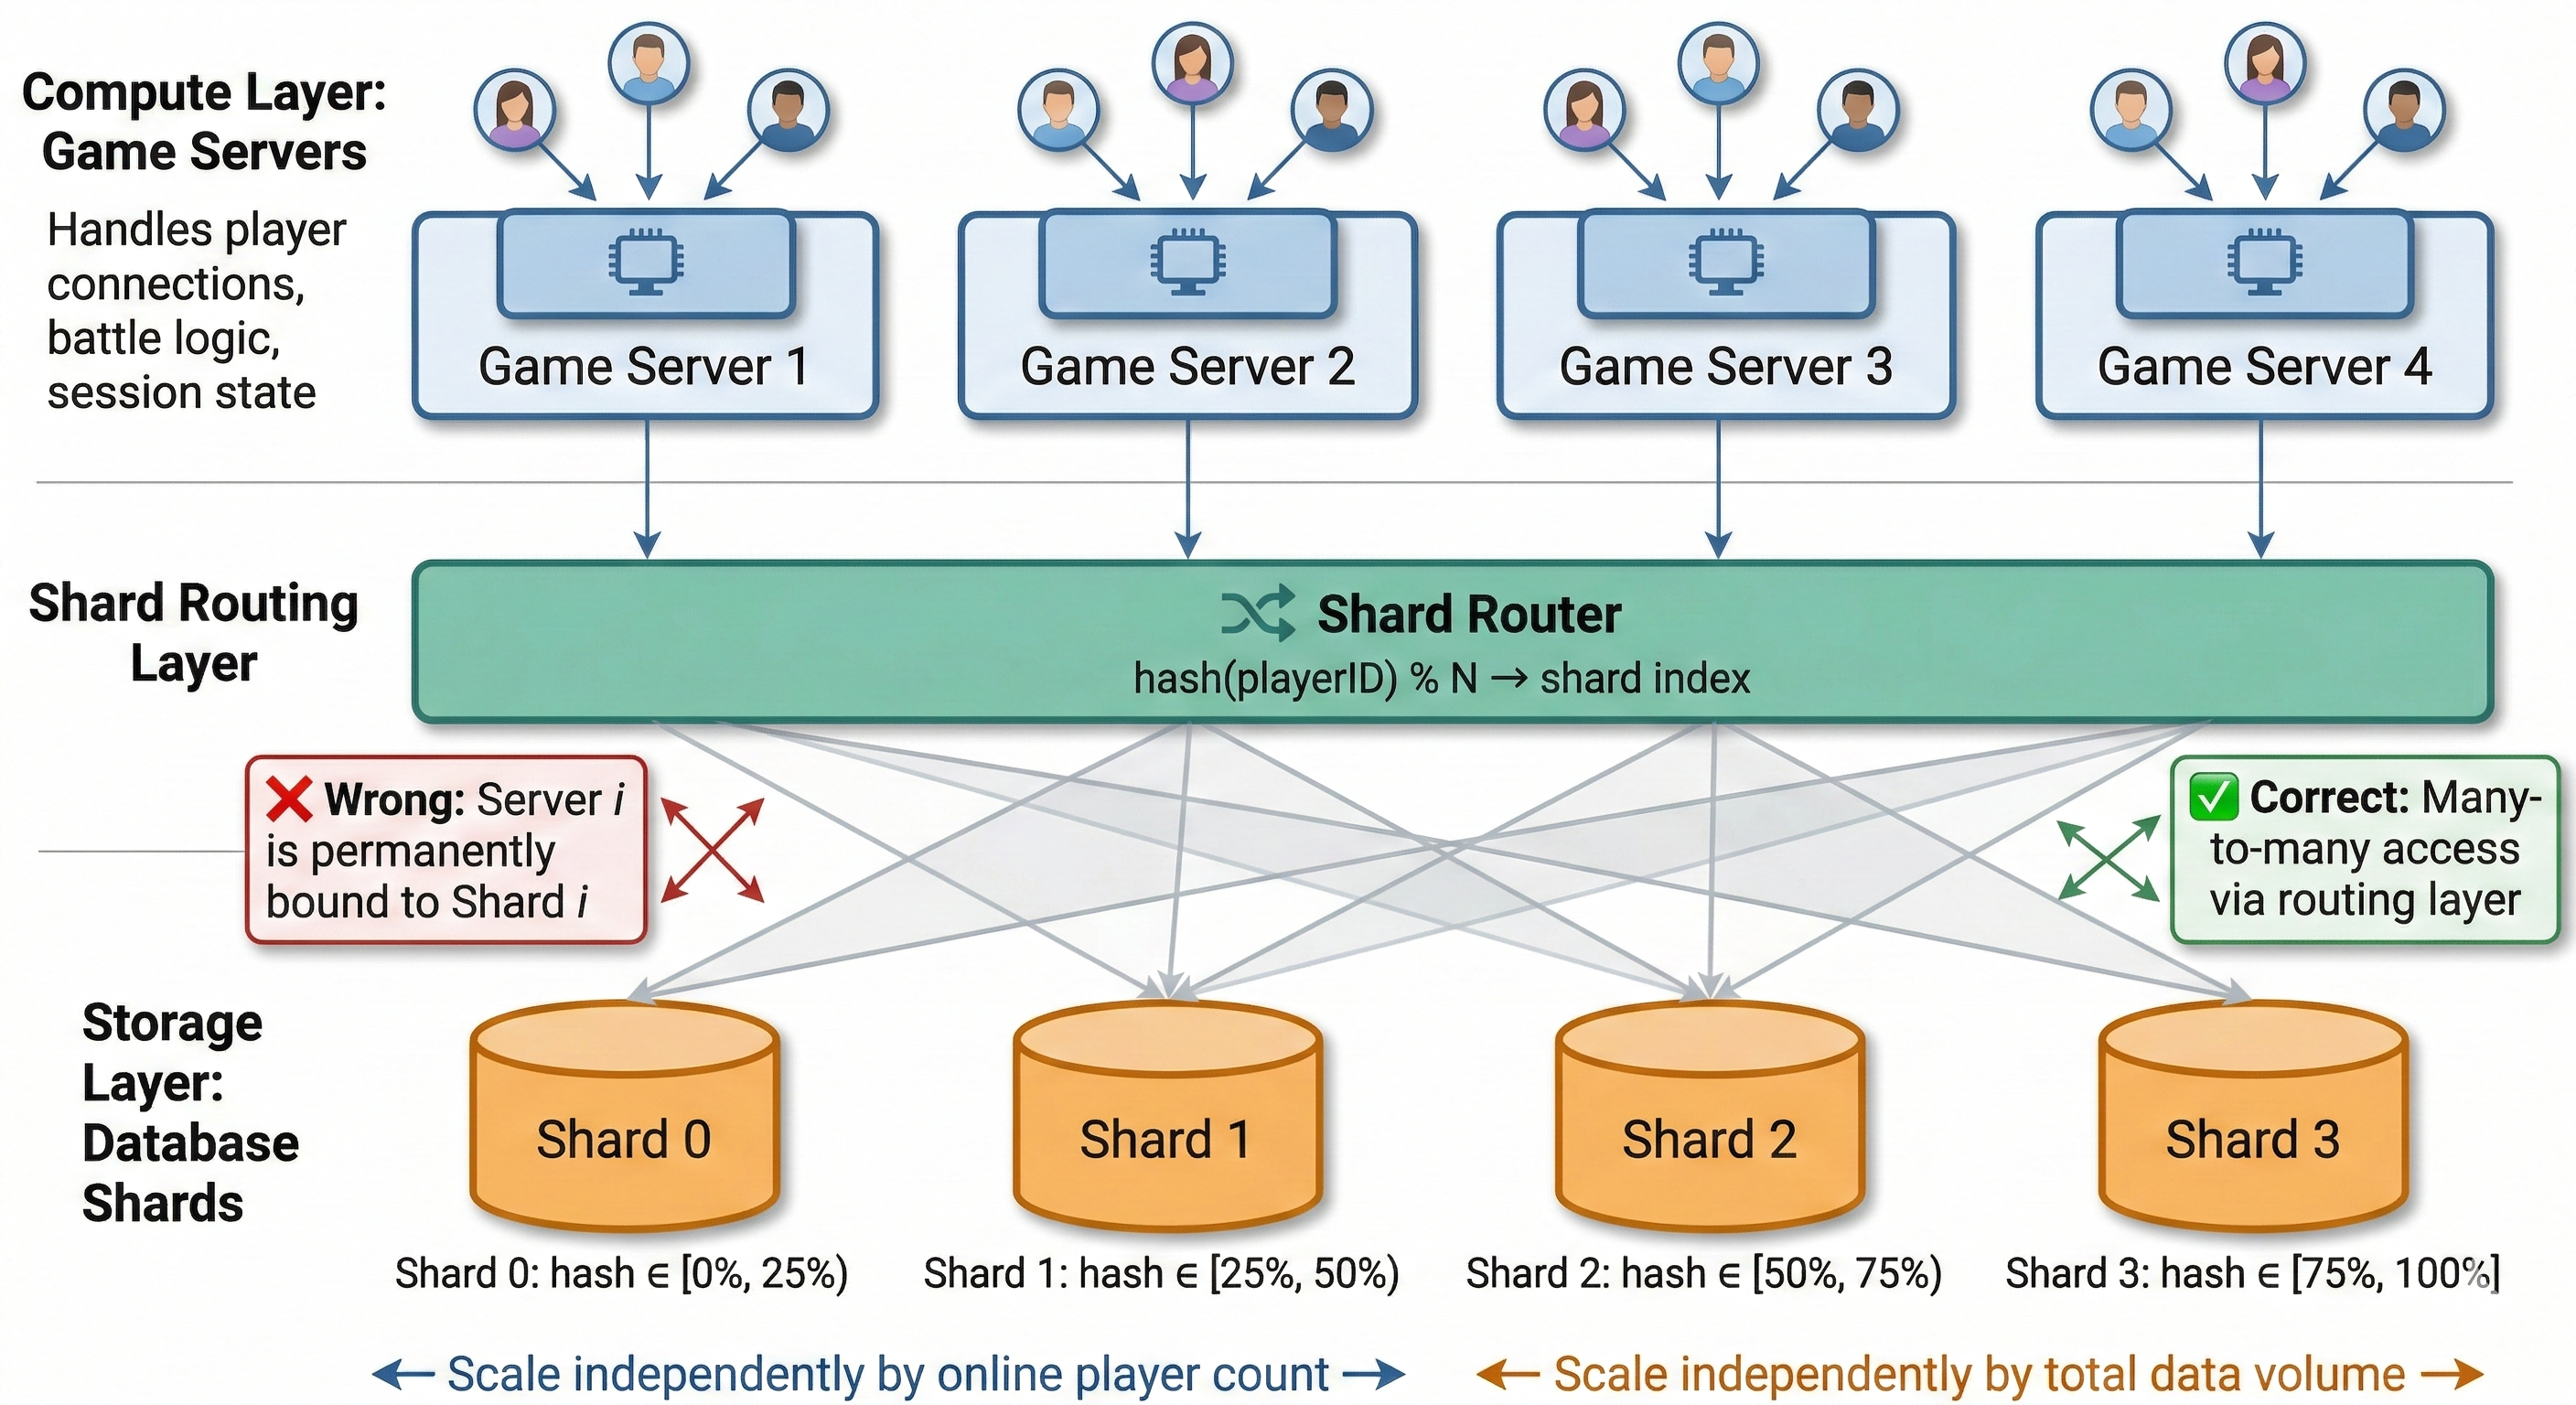
\includegraphics[width=1\linewidth]{figures/sec4/4-server-db.png}
    \caption{游戏服务器（计算层）与数据库分片（存储层）的解耦关系：
    任意游戏服务器均可经由分片路由层访问任意数据库分片，
    两层按各自压力独立水平扩展，不存在一一绑定关系}
    \label{fig:server_db_relationship}
\end{figure}

明确了计算层与存储层的解耦关系之后，计算层扩展的核心问题便清晰地浮现出来：
当我们部署了多台游戏服务器之后，如何让每一台服务器都承担合适的玩家数量和计算压力，
而不是有的服务器人满为患、有的服务器门可罗雀？这正是负载均衡要解决的核心问题。
负载均衡器作为计算层的入口，承担着与分片路由层对等的角色：
分片路由层决定"一条数据库请求去往哪个分片"，
负载均衡器则决定"一个玩家的连接请求去往哪台游戏服务器"。
两者共同构成了整个分布式游戏系统中的两级路由体系，分别守护着存储层和计算层的入口。


\subsubsection{负载不均的表现与根源}

从玩家的视角看，负载不均衡通常表现为两个极端。一方面，有的游戏区服在登录时总是排队，玩家点击"进入游戏"后会看到"当前服务器繁忙，排队中...前方还有 XXX 人"的提示，等待数分钟才能进入；即使成功登录，进入游戏后也感觉卡顿明显——点击匹配按钮后要等很久才能找到对手，战斗过程中画面偶尔会停顿，战斗结算慢，有时甚至会出现"操作超时"的错误提示。另一方面，另一些区服则人迹罕至，玩家登录几乎不需要等待，但进入游戏后发现世界频道冷冷清清，几分钟都没人说话，想要匹配对手时系统提示"当前在线人数较少，匹配时间可能较长"，等了十几分钟也没匹配到人，只能放弃。

这种体验上的巨大差异，归根结底是因为服务器资源没有被合理利用。把这种现象翻译到服务器背后，可以看到一个简单但严重的事实：不同的游戏服务器承载的玩家数量和计算负载差异巨大。假设我们部署了五台游戏服务器，理想情况下每台服务器应该承载大约 20\% 的在线玩家，CPU 使用率都在 60\% 左右，响应时间都在 100 毫秒以内。但现实往往是：服务器 1 承载了 40\% 的玩家，CPU 使用率常年在 90\% 以上，内存占用接近上限，平均响应时间超过 500 毫秒，玩家感受到明显的卡顿；服务器 2 和服务器 3 各承载了 20\% 的玩家，运行状态正常；服务器 4 只有 15\% 的玩家，CPU 使用率只有 40\%，还有大量闲置资源；服务器 5 更是只有 5\% 的玩家，几乎处于空转状态，每天大部分时间都在等待请求。

造成这种不均衡的原因是多方面的。开服时间的差异是最常见的一种：服务器 1 可能是游戏刚上线时开的第一批服务器，大量早期玩家都注册在这个服务器上，形成了庞大的玩家基数和成熟的社交网络；即使后来开了新服务器，老玩家也不愿意迁移，因为他们在老服上有朋友、有公会、有积累。社区效应也会加剧这种不均衡：某个知名主播或游戏公会宣布在服务器 1 上活动，吸引了大量粉丝和玩家涌入；又或者某个服务器因为运气好、氛围好，在玩家社区中形成了"这个服人气旺、高手多"的口碑，进一步吸引新玩家加入，形成正反馈循环。还有技术层面的失误：在没有负载均衡机制的情况下，玩家选服时看到的服务器列表可能是按开服时间或名称排序的，很多玩家会习惯性地选择列表中的第一个或最上面的服务器，导致某几个服务器被优先填满。

这种不均衡不仅造成了资源浪费——服务器 4 和服务器 5 的硬件闲置率极高，相当于花钱买了机器却没有充分使用——更严重的是，它直接影响了玩家的游戏体验。在过载的服务器上，玩家忍受着糟糕的性能；在冷清的服务器上，玩家感受不到多人游戏应有的社交氛围和竞技乐趣。长此以往，过载服务器的玩家会因为体验太差而流失，冷清服务器的玩家会因为找不到对手而离开，最终两边都留不住玩家。

负载均衡的目标，就是通过科学的流量调度策略，让每一台游戏服务器都处于一个相对均衡的工作状态，既不至于过载崩溃，也不会过度闲置。可以把负载均衡器想象成一个站在"入口大厅"的智能引导员：所有新登录的玩家都先来到这个入口，引导员手里有一张实时更新的"服务器状态表"，记录着每台服务器当前的在线人数、CPU 使用率、内存占用、平均响应时间等信息；当一个新玩家到来时，引导员快速查看这张表，找出当前负载最轻、最适合接纳新玩家的服务器，然后将这个玩家的连接请求转发到那台服务器上。整个过程对玩家来说是透明的——玩家只知道自己点击了"开始游戏"，几秒钟后就进入了游戏世界，并不知道背后经历了负载均衡器的选择和转发。

\subsubsection{从轮询到动态调度的策略演进}

要实现负载均衡，最直接的想法是采用轮询策略。假设我们有三台游戏服务器 A、B、C，负载均衡器维护一个简单的计数器，按照固定顺序依次分配玩家：第一个玩家分配到 A，计数器加 1；第二个玩家分配到 B，计数器加 1；第三个玩家分配到 C，计数器加 1；第四个玩家再回到 A，计数器归零后重新开始循环，如此往复。

\begin{tcolorbox}[title=轮询策略的核心逻辑]
\begin{lstlisting}[
    language=go,
    basicstyle=\ttfamily\footnotesize,
    aboveskip=0pt, belowskip=0pt,
    lineskip=-1pt,
    commentstyle=\color{gray},
    keywordstyle=\color{blue}\bfseries,
    breaklines=true
]
// 选择下一个服务器（轮询）
current = (current + 1) % numServers
return servers[current]
\end{lstlisting}
\end{tcolorbox}

这种策略的优点在于规则清晰、实现简单，代码量很少，逻辑一目了然，不需要收集任何服务器的实时状态信息，不需要复杂的计算和判断。而且从统计学的角度看，如果玩家登录是随机分布的，经过足够长的时间，每台服务器理论上都会接收到大致相同数量的新玩家——假设有 10000 个玩家陆续登录，三台服务器最终各自会分配到约 3333 个玩家，偏差不会太大。

但轮询策略有一个明显的局限：它只关心"过去分配了多少人"，而完全不关心"现在每台服务器到底有多忙"。这种"盲目"的分配方式在某些情况下会导致严重的问题。假设服务器 A 因为历史原因已经承载了 5000 个老玩家，这些老玩家虽然没有在刚才的轮询分配中被计入，但他们确实占用着服务器 A 的 CPU、内存和网络资源。此时，如果继续按照轮询规则将新玩家平均分配给三台服务器，服务器 A 就会承受双重压力：5000 个老玩家加上新分配来的约 3333 个新玩家，总共 8333 个玩家；而服务器 B 和 C 可能只有新分配的 3333 个玩家。结果是服务器 A 的负载远高于 B 和 C，性能急剧下降，玩家体验变差。

更极端的情况是，某台服务器正在处理突发的高负载事件。比如，服务器 A 上的两个大型公会正在进行一场 100 人规模的公会战，这场战斗涉及大量的位置同步、技能计算、伤害结算，CPU 使用率已经飙升到 95\%，响应时间从平时的 50 毫秒增加到了 800 毫秒。但轮询策略对这一切毫无感知，它仍然会按照固定的顺序，将下一批新登录的玩家中的三分之一分配给服务器 A。这些新玩家刚登录就会感受到明显的延迟和卡顿，甚至可能因为服务器过载而连接失败。与此同时，服务器 B 和 C 可能相对空闲，CPU 使用率只有 30\%，完全有余力接纳更多玩家，但轮询策略并不会将更多玩家导向它们。

为了克服这个问题，我们需要让负载均衡器具备"感知"能力——它需要知道每台服务器当前的真实负载状况，并根据这些信息做出更智能的分配决策。具体做法是让每台游戏服务器定期向负载均衡器报告自己的当前状态，这个报告过程通常通过心跳机制来实现：每台游戏服务器每隔一段时间（比如每 5 秒）向负载均衡器发送一条心跳消息，消息中包含该服务器的关键指标，包括在线玩家数、CPU 使用率、内存占用率、平均响应时间、当前活跃战斗数等。

\begin{tcolorbox}[title=服务器心跳上报的关键数据]
\begin{lstlisting}[
    language=go,
    basicstyle=\ttfamily\footnotesize,
    aboveskip=0pt, belowskip=0pt,
    lineskip=-1pt,
    commentstyle=\color{gray},
    keywordstyle=\color{blue}\bfseries,
    breaklines=true
]
type ServerStatus struct {
    ServerID      string
    OnlinePlayers int     // 在线玩家数
    CPUUsage      float64 // CPU使用率 (0-100)
    MemUsage      float64 // 内存使用率 (0-100)
    AvgRespTime   int     // 平均响应时间（毫秒）
    ActiveBattles int     // 活跃战斗数
}
// 每5秒发送一次心跳到负载均衡器
\end{lstlisting}
\end{tcolorbox}

负载均衡器收集到这些信息之后，会在内存中维护一张"服务器状态表"，记录每台服务器的最新状态。游戏服务器启动时会创建一个定时器，每隔固定时间间隔读取自身的运行指标，将这些指标打包成一条消息发送给负载均衡器；负载均衡器收到心跳后，更新对应服务器在状态表中的记录，并记录心跳的接收时间，用于后续的健康检查。

有了这些实时状态信息，负载均衡器就可以做出更明智的决策。最简单的一种动态策略是"最少连接优先"：负载均衡器会优先将新玩家分配到当前在线玩家数最少的服务器上。这种策略的直觉很简单——玩家数少的服务器通常意味着负载较轻，还有余力接纳更多玩家；而玩家数多的服务器可能已经接近满负载，不应该继续向它分配新玩家。实现时，负载均衡器在收到新玩家的连接请求后，遍历服务器状态表，找出在线玩家数最少的那台服务器，将玩家的连接转发给它。

最少连接策略相比轮询策略有了显著的改进。当某台服务器因为历史原因积累了大量玩家时，负载均衡器会自动减少向它分配新玩家，转而将更多新玩家导向那些相对空闲的服务器，从而实现负载的动态平衡。随着时间推移，各台服务器的玩家数量会逐渐趋于一致，不再出现某台服务器人满为患、另一台服务器门可罗雀的极端情况。

但"最少连接"也不是万能的。玩家数量并不总是等同于计算负载，这是一个非常重要但容易被忽视的事实。我们可以构造这样一个场景来说明问题：服务器 A 当前在线 2000 个玩家，服务器 B 当前在线 3000 个玩家。从玩家数量上看，服务器 A 明显更少，按照最少连接策略，下一个玩家应该被分配到服务器 A。但实际情况可能是：服务器 A 上的 2000 个玩家中有 1500 个正在进行激烈的实时对战，每场战斗都需要频繁的位置同步、技能判定、伤害计算，CPU 使用率已经达到 85\%；而服务器 B 上的 3000 个玩家中有 2000 个处于挂机状态（可能在等待体力恢复、在城镇闲逛、或者打开了游戏但没有实际操作），只有 1000 个在进行战斗，CPU 使用率只有 50\%。在这种情况下，如果继续将新玩家分配给服务器 A，很可能导致它过载；而服务器 B 虽然玩家更多，但实际上还有充足的计算资源可以接纳更多玩家。

这个例子揭示了一个关键问题：玩家数量是一个简单但粗糙的指标，它无法准确反映服务器的真实负载。要做出更精准的负载评估，我们需要综合考虑多个维度的指标：在线玩家数（反映需要维护的连接数和会话状态数量）、CPU 使用率（反映计算压力，战斗计算、路径寻找、AI 决策等都会消耗 CPU）、内存占用率（反映内存使用情况，过高可能触发系统回收机制）、平均响应时间（反映整体性能表现，是玩家最直接感受到的指标）、活跃战斗数（反映当前的业务负载强度，在对战游戏中这是计算密集型任务）。

我们可以为每个指标设置一个权重，然后将各个指标的数值按权重加总，得到一个综合负载值。权重的设置需要根据具体的游戏特性和硬件配置来调整。例如，对于我们的对战游戏，战斗计算是主要的性能瓶颈，CPU 使用率和活跃战斗数应该占更高的权重；而对于社交类游戏，在线玩家数和网络带宽可能更重要。

\begin{tcolorbox}[title=综合负载值的计算方法]
\begin{lstlisting}[
    language=go,
    basicstyle=\ttfamily\footnotesize,
    aboveskip=0pt, belowskip=0pt,
    lineskip=-1pt,
    commentstyle=\color{gray},
    keywordstyle=\color{blue}\bfseries,
    breaklines=true
]
// 计算综合负载值（0-100，值越高负载越重）
loadScore = playerScore*0.2 + cpuScore*0.3 + memScore*0.2 
          + respTimeScore*0.2 + battleScore*0.1

// 选择负载最低的服务器
bestServer = findMinLoadScore(allServers)
\end{lstlisting}
\end{tcolorbox}

计算时，首先将各项指标归一化到 0-100 的范围（比如假设 5000 人为玩家数满载，1000 毫秒为严重延迟的响应时间），然后按照预设的权重进行加权求和，最终得到一个 0-100 的综合负载值，数值越高表示负载越重。负载均衡器在分配玩家时，选择综合负载值最低的服务器。

通过这种加权负载评估，负载均衡器可以更全面地了解每台服务器的真实状况。即使某台服务器的在线玩家数较少，但如果它的 CPU 使用率很高、活跃战斗数很多，综合负载值仍然会比较高，负载均衡器就不会继续向它分配新玩家；相反，如果另一台服务器虽然玩家数较多，但大部分玩家处于空闲状态，各项指标都比较健康，综合负载值较低，负载均衡器就会优先将新玩家分配给它。

% \begin{figure}[htbp]
%     \centering
%     % 图片描述：不同负载均衡策略的对比示意图
%     % 三个子图水平排列：
%     % 左图：轮询策略
%     %   - 三台服务器A、B、C的柱状图，高度相同（各33.3%）
%     %   - 标注"平均分配，但未考虑实际负载"
%     % 中图：最少连接策略
%     %   - 三台服务器的柱状图，高度根据玩家数动态调整
%     %   - 服务器A: 40%（老玩家多），服务器B: 35%，服务器C: 25%（新开服）
%     %   - 标注"根据玩家数动态调整"
%     % 右图：加权负载策略
%     %   - 三台服务器的柱状图，高度根据综合负载值调整
%     %   - 每个柱子分段显示不同指标的贡献（CPU、内存、玩家数等）
%     %   - 服务器A综合负载85分，服务器B: 60分，服务器C: 45分
%     %   - 标注"多维度综合评估"
%     % 所有文字使用简体中文
%     \caption{不同负载均衡策略的分配效果对比}
%     \label{fig:load_balancing_comparison}
% \end{figure}

\subsubsection{硬件差异与动态权重}

在实际部署中，还有一个现实问题需要考虑：不同的游戏服务器可能拥有不同的硬件配置。在游戏运营的早期阶段，我们可能只有几台配置一般的服务器（比如 8 核 CPU、32GB 内存）；随着玩家增长，我们陆续采购了一些性能更强的服务器（比如 16 核 CPU、64GB 内存）；到了后期，可能还会租用云服务器，这些云服务器的配置可能又各不相同。如果采用完全均等的负载均衡策略，不考虑硬件差异，就会导致一个问题：配置较低的服务器更容易过载，而配置较高的服务器则没有充分发挥性能优势。

假设服务器 A 是老旧的 8 核服务器，承载能力大约是 2000 个并发玩家；服务器 B 是新购的 16 核服务器，承载能力大约是 4000 个并发玩家。如果负载均衡器简单地将玩家平均分配，最终两台服务器各承载 3000 个玩家，结果就是：服务器 A 严重过载（超出承载能力 50\%），CPU 使用率常年在 95\% 以上，玩家体验很差；而服务器 B 还有余力（只用了 75\% 的承载能力），但由于负载均衡器的限制，没能接纳更多玩家。

为了解决这个问题，我们可以为每台服务器设置一个权重值。权重值通常根据服务器的硬件配置来确定，配置越高、承载能力越强的服务器，权重值越大。负载均衡器在分配玩家时，会按照权重比例进行分配，让硬件资源得到更充分的利用。例如，如果服务器 A（8 核）权重设为 1，服务器 B（16 核）权重设为 2，服务器 C（24 核）权重设为 3，那么在长期运行中，三台服务器接收到的玩家数量会大致符合 1:2:3 的比例，服务器 A 接收约 16.7\% 的流量，服务器 B 接收约 33.3\%，服务器 C 接收约 50\%。通过权重机制，我们可以让高配置服务器承担更多的玩家，低配置服务器承担较少的玩家，使得每台服务器都工作在合理的负载水平上，既不会因为配置低而过载，也不会因为配置高而闲置。

但权重也不应该是固定不变的。随着服务器运行时间的增长，硬件可能会老化，性能有所下降；或者某台服务器上积累了大量的历史数据（比如战斗记录、聊天日志），导致数据库查询变慢；又或者某台服务器因为网络拓扑的原因，与部分玩家之间的延迟较高。这些因素都会影响服务器的实际承载能力。因此，更好的做法是引入动态权重调整机制：负载均衡器不仅在启动时从配置中读取静态权重，还会根据服务器的实时表现动态调整权重。如果某台服务器虽然硬件配置高，但实际表现不佳（比如平均响应时间持续偏高），负载均衡器会逐步降低它的权重，减少向它分配的流量；反之，如果某台服务器表现优异，权重可以适当提升。调整的方式可以是：每次收集到服务器状态信息后，根据综合负载值与目标负载值的差距，微调该服务器的权重——如果综合负载持续高于目标值，权重逐步下降；如果持续低于目标值，权重逐步上升。这种微调是渐进的、平滑的，避免权重的剧烈波动导致流量分配不稳定。

\subsubsection{健康检查与故障隔离}

除了动态权重，负载均衡器还需要建立健康检查机制。所谓健康检查，就是负载均衡器定期向每台游戏服务器发送探测请求，检测服务器是否正常响应。这个探测可以是一个简单的 HTTP 请求（比如访问一个专门的健康检查端点），也可以是一个轻量级的 RPC 调用。服务器收到探测请求后，应该快速返回一个包含自身状态信息的响应，表明自己还活着并且运行正常。响应中不仅包含一个简单的"我还活着"的标志，还可以包含一些关键指标的快照，比如当前 CPU 使用率、是否能正常连接数据库、是否有严重的错误日志等。

如果某台服务器连续多次健康检查失败——可能是进程崩溃、可能是网络中断、可能是硬件故障——负载均衡器就会将这台服务器标记为"不可用"，暂停向它分配新玩家。这个标记过程通常会设置一个失败次数阈值，避免因为偶发的网络抖动而误判。比如，只有当连续三次健康检查都失败时，才将服务器标记为不可用；而当服务器恢复正常、连续三次健康检查都成功时，才将它重新标记为可用。标记为不可用的服务器会被从分配池中移除，新玩家的连接请求不会再被转发到这台服务器，所有流量都会被导向其他健康的服务器。

对于已经连接到故障服务器的玩家，负载均衡器还需要考虑如何处理。最简单的做法是让这些玩家的连接自然断开，等他们重新登录时再分配到其他健康的服务器上。但这种方式对玩家体验影响较大——正在进行战斗的玩家会突然掉线，正在浏览背包的玩家会看到"连接丢失"的错误。更好的做法是引入连接迁移机制：当负载均衡器检测到某台服务器不健康时，会向该服务器上的所有玩家发送一条"服务器维护"的通知，引导他们在未来的某个时间点（比如当前战斗结束后、或者 5 分钟后）重新连接到其他服务器。这样可以给玩家一个缓冲期，避免突然的连接中断。待故障服务器恢复正常后，负载均衡器会重新将其纳入分配池。但不应该立即将大量玩家分配给刚恢复的服务器，因为它可能还处于不稳定状态，或者需要时间来预热（比如加载缓存、建立数据库连接池等）。更稳妥的做法是逐步恢复：刚恢复时，只分配少量玩家；观察一段时间后，如果服务器表现稳定，再逐步增加分配的流量，直到恢复到正常的权重比例。

\subsubsection{运行时动态迁移应对突发负载}

负载均衡不仅仅发生在玩家刚登录的那个瞬间。在游戏运行过程中，各台服务器的负载可能因为各种
原因发生剧烈波动。最典型的情况是突发事件：某个服务器上正在举行一场大型公会战，
参战的 200 个玩家几乎同时上线并进入战场，短时间内该服务器的活跃战斗数从 50 场飙升到 150 场，
CPU 使用率从平时的 50\% 跃升到 90\%，平均响应时间从 100 毫秒增加到 600 毫秒。
与此同时，另一些服务器可能相对空闲——也许是因为时区差异导致欧洲玩家还没上线，
也许只是这一批玩家碰巧都在做日常任务、没人打排位赛。
如果仅靠"不再向过载服务器分配新玩家"这一策略，只能防止问题进一步恶化，
但无法缓解已经发生的过载——过载服务器上那批老玩家还在继续游戏，CPU 仍然居高不下。
为此，一些高级的负载均衡系统会引入运行时的动态迁移机制，
主动将过载服务器上的部分玩家迁移到相对空闲的服务器上。

动态迁移的第一个问题是"迁移谁"。并不是所有玩家都适合在运行时被迁移——
正在战斗中的玩家、正在进行购买或开箱等关键操作的玩家，迁移会打断他们的状态，
造成不良体验甚至数据丢失。更合适的迁移对象是那些暂时不活跃的玩家：
超过 10 分钟没有任何操作的挂机玩家、刚结束战斗正在查看战绩的玩家、
在城镇闲逛或浏览商店的玩家。这些玩家当前的游戏状态较为简单，
迁移时需要同步的数据量小，中断带来的影响也最轻微。

动态迁移的第二个、也是更核心的问题是"怎么迁移"。
这里所说的迁移，并非重启连接这么简单——玩家登录游戏后，
服务器内存中保存着他当前的完整游戏状态：角色在地图上的位置、当前血量和技能冷却、
进行中的任务进度、战斗中的仇恨列表，乃至玩家客户端的网络连接上下文。
如果只是断开连接然后让玩家重新登录，固然可行，但玩家体验很差——
相当于强制把玩家踢出再拉回来。真正的状态热迁移要求：在玩家几乎无感知的前提下，
将这份内存中的活跃状态完整地搬到另一台服务器上，并由目标服务器无缝接管后续的服务。
根据如何处理"迁移期间源服务器仍在运行、状态仍在变化"这一核心矛盾，
主要有以下三种方案，复杂度和效果依次递进。

\paragraph{方案一：停止复制法（Stop-and-Copy）}

最直接的做法是"先停、再搬、再启"，即停止复制法（Stop-and-Copy），
如图~\ref{fig:migration_stop_copy} 所示。
迁移开始时，源服务器立即停止处理该玩家的所有请求，
将玩家的完整会话状态序列化为一个可传输的数据结构，
通过网络传输到目标服务器，目标服务器反序列化后恢复玩家会话，
最后原服务器关闭连接，玩家的客户端重连到目标服务器。
这种方案的优点是实现极为简单：停机期间状态不再变化，不存在任何数据竞争，
序列化的快照完全一致，目标服务器恢复时无需任何额外协调。
缺点也同样明显：玩家在整个传输过程中处于完全停服状态，
停机时长与需要迁移的状态数据量成正比——
对于一个状态复杂的玩家（身处大型公会战、同屏数十个技能特效全部需要同步），
全量序列化和传输可能耗时数秒甚至更长，玩家会明显看到"连接断开"或"转圈等待"。
因此，停止复制法通常只适用于离线维护窗口或玩家处于彻底挂机状态的场景，
不适合作为生产环境中的主动负载均衡手段。

\begin{figure}[htbp]
    \centering
    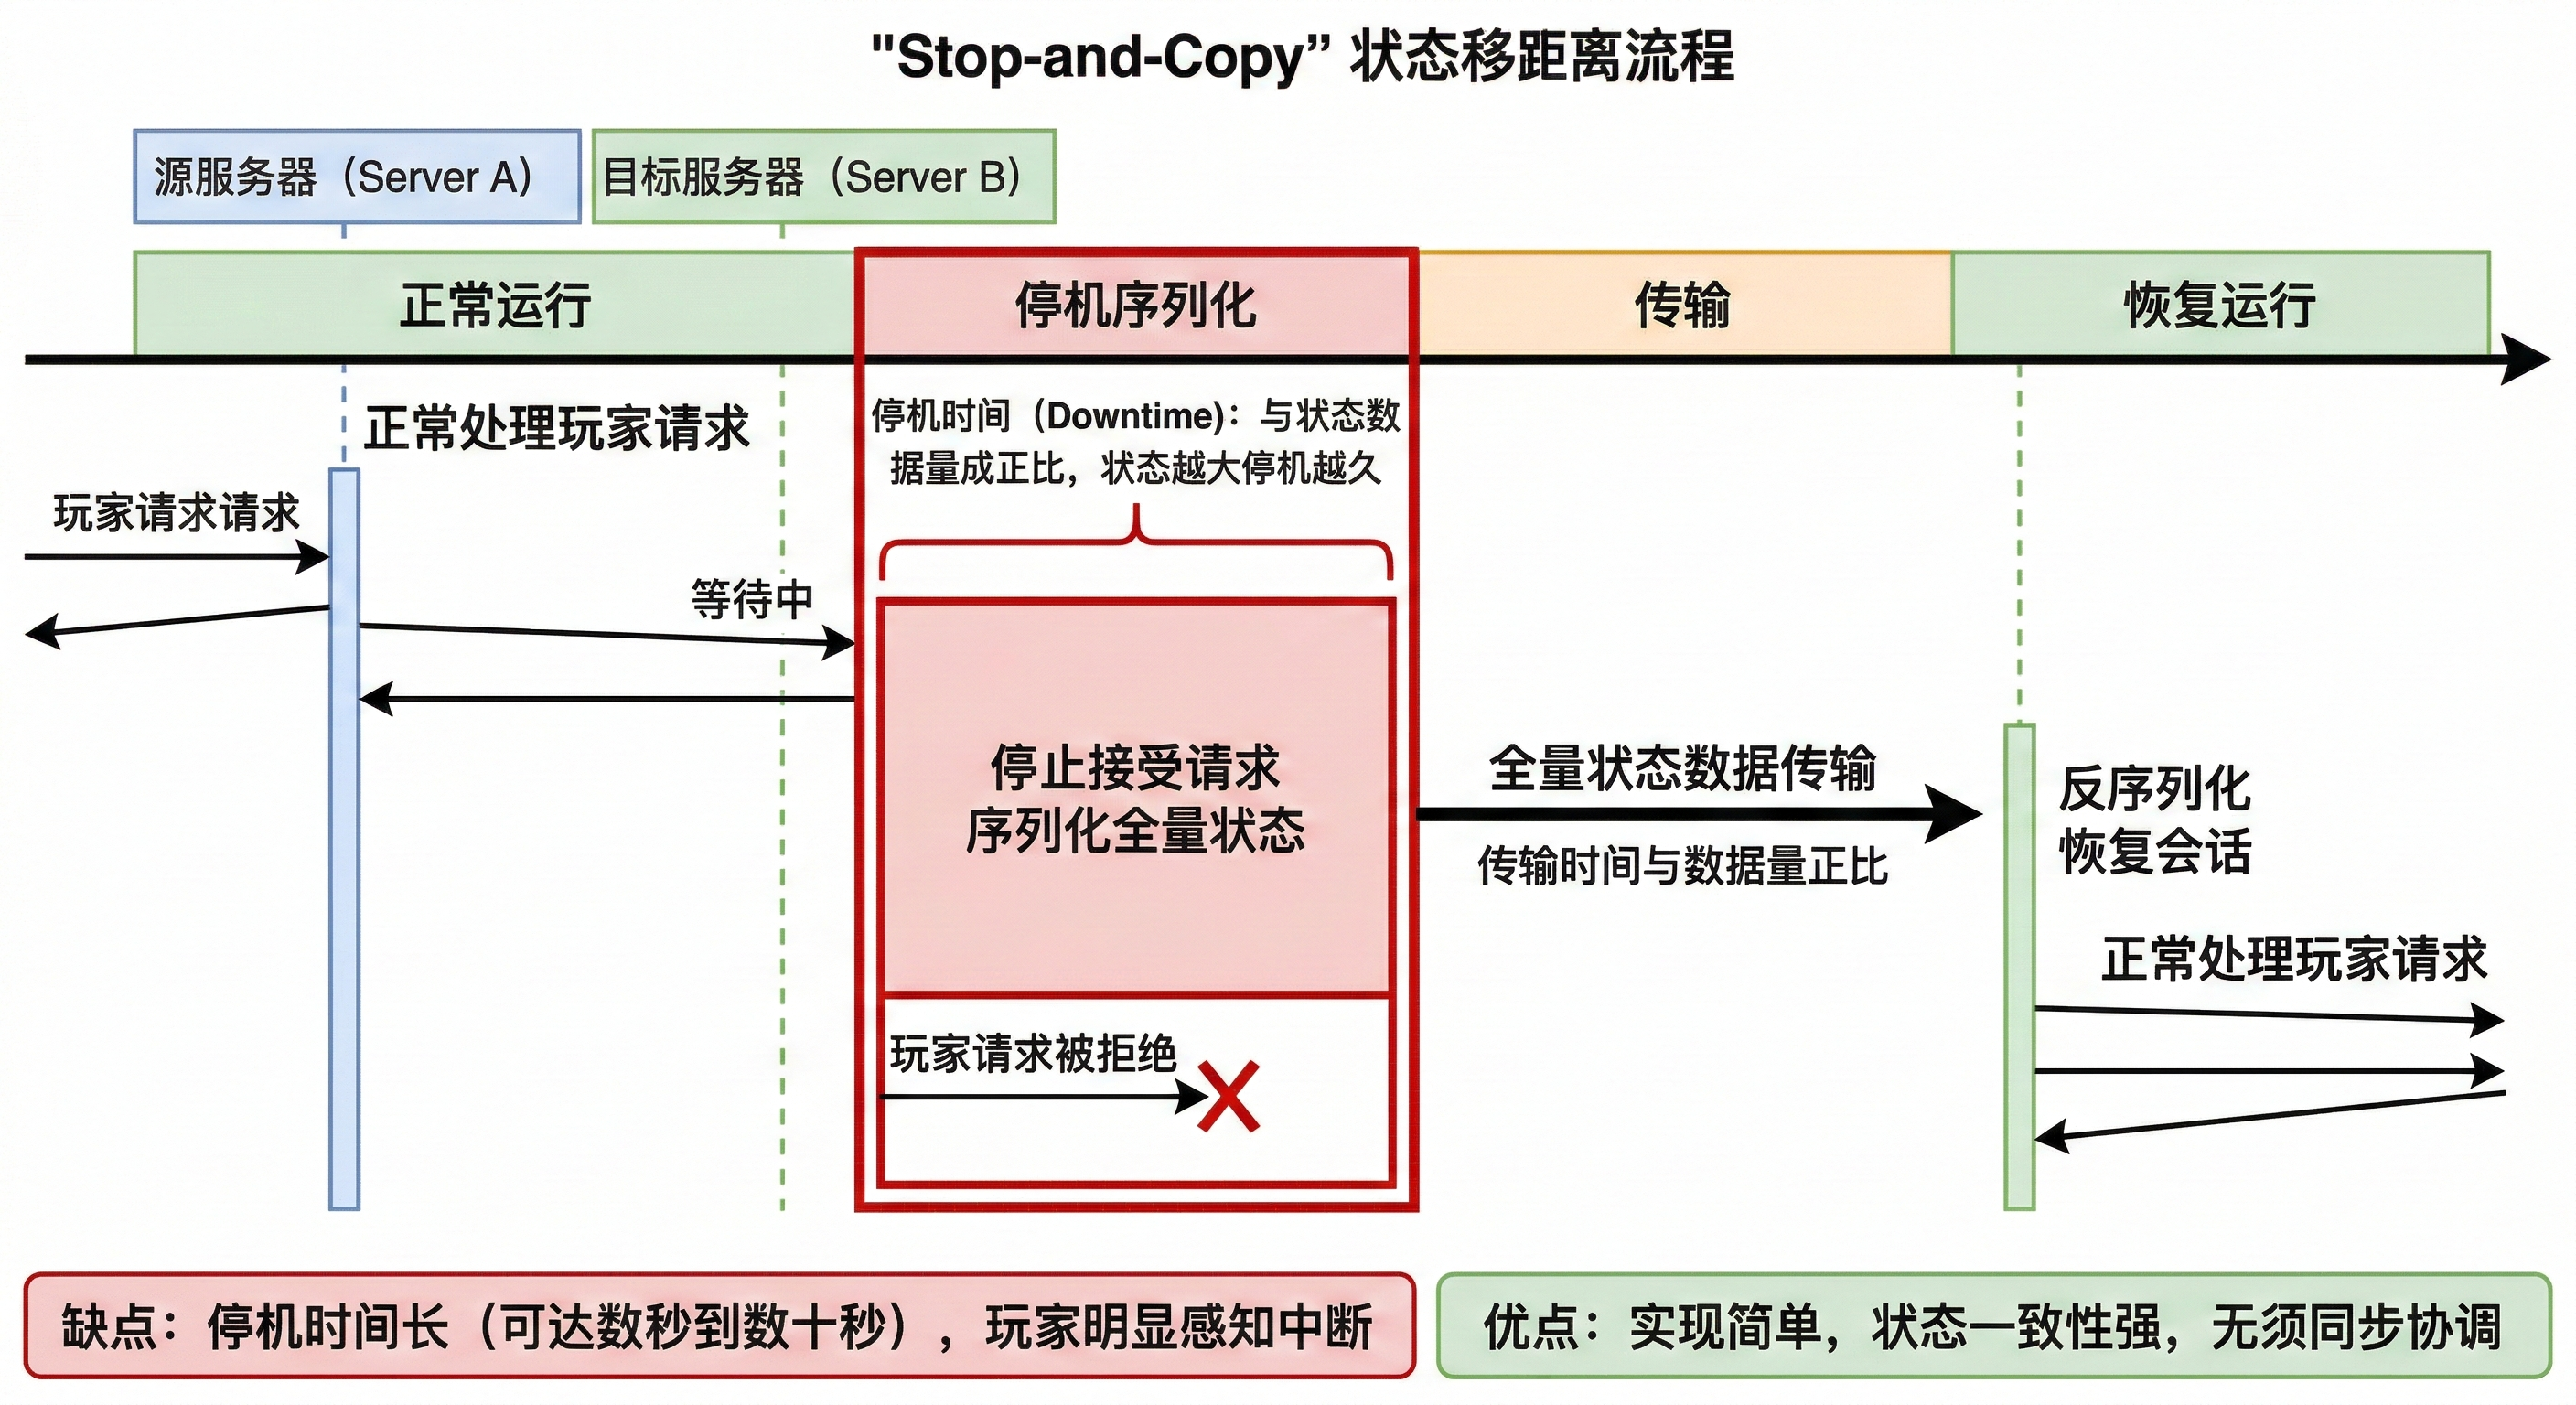
\includegraphics[width=1\linewidth]{figures/sec4/4-migrate-stop.png}
    \caption{停止复制法（Stop-and-Copy）：源服务器停机后传输全量状态，
    停机时间与状态数据量成正比，玩家会明显感知到连接中断}
    \label{fig:migration_stop_copy}
\end{figure}

\paragraph{方案二：预复制法（Pre-Copy）}

为了缩短玩家感知到的停机时间，可以把大部分数据的传输提前到停机之前完成，
这就是预复制法（Pre-Copy），如图~\ref{fig:migration_precopy} 所示。
其核心思路是：在源服务器仍然运行的同时，持续地将玩家状态的内存快照传输到目标服务器；
每一轮传输结束后，追踪本轮期间哪些内存页被修改过（称为"脏页"，Dirty Pages），
再在下一轮只传输这些脏页，逐轮迭代，直到每轮的脏页数量收敛到足够小；
最后才进行一次极短暂的停机，将最后一批脏页和 CPU 寄存器状态传输过去，
完成最终切换。
这里有个关键直觉值得理解：游戏服务器的内存并不会在每一秒内把所有状态全部修改一遍，
绝大多数玩家数据（已完成的任务记录、背包里不在使用的装备、离线好友列表等）
在单次传输间隔内根本不会被修改，只有当前正在活跃变化的那部分状态（当前帧的位置、血量）
才会产生新的脏页。随着迭代轮次增加，每轮需要重传的脏页越来越少，
最终只需在极短的窗口内传输最后一批脏页就能完成切换，
停机时间通常可以从秒级压缩到百毫秒级甚至更低。
预复制法的代价是总传输量会超过全量状态大小——部分脏页在多轮迭代中被反复传输，
网络带宽的消耗高于停止复制法；对于那些高频修改的"热页"（比如每帧都在变化的角色位置），
无论迭代多少轮都无法在停机前完全收敛，最终仍然要在停机阶段传输，
这构成了预复制法停机时间的理论下界。

\begin{figure}[htbp]
    \centering
    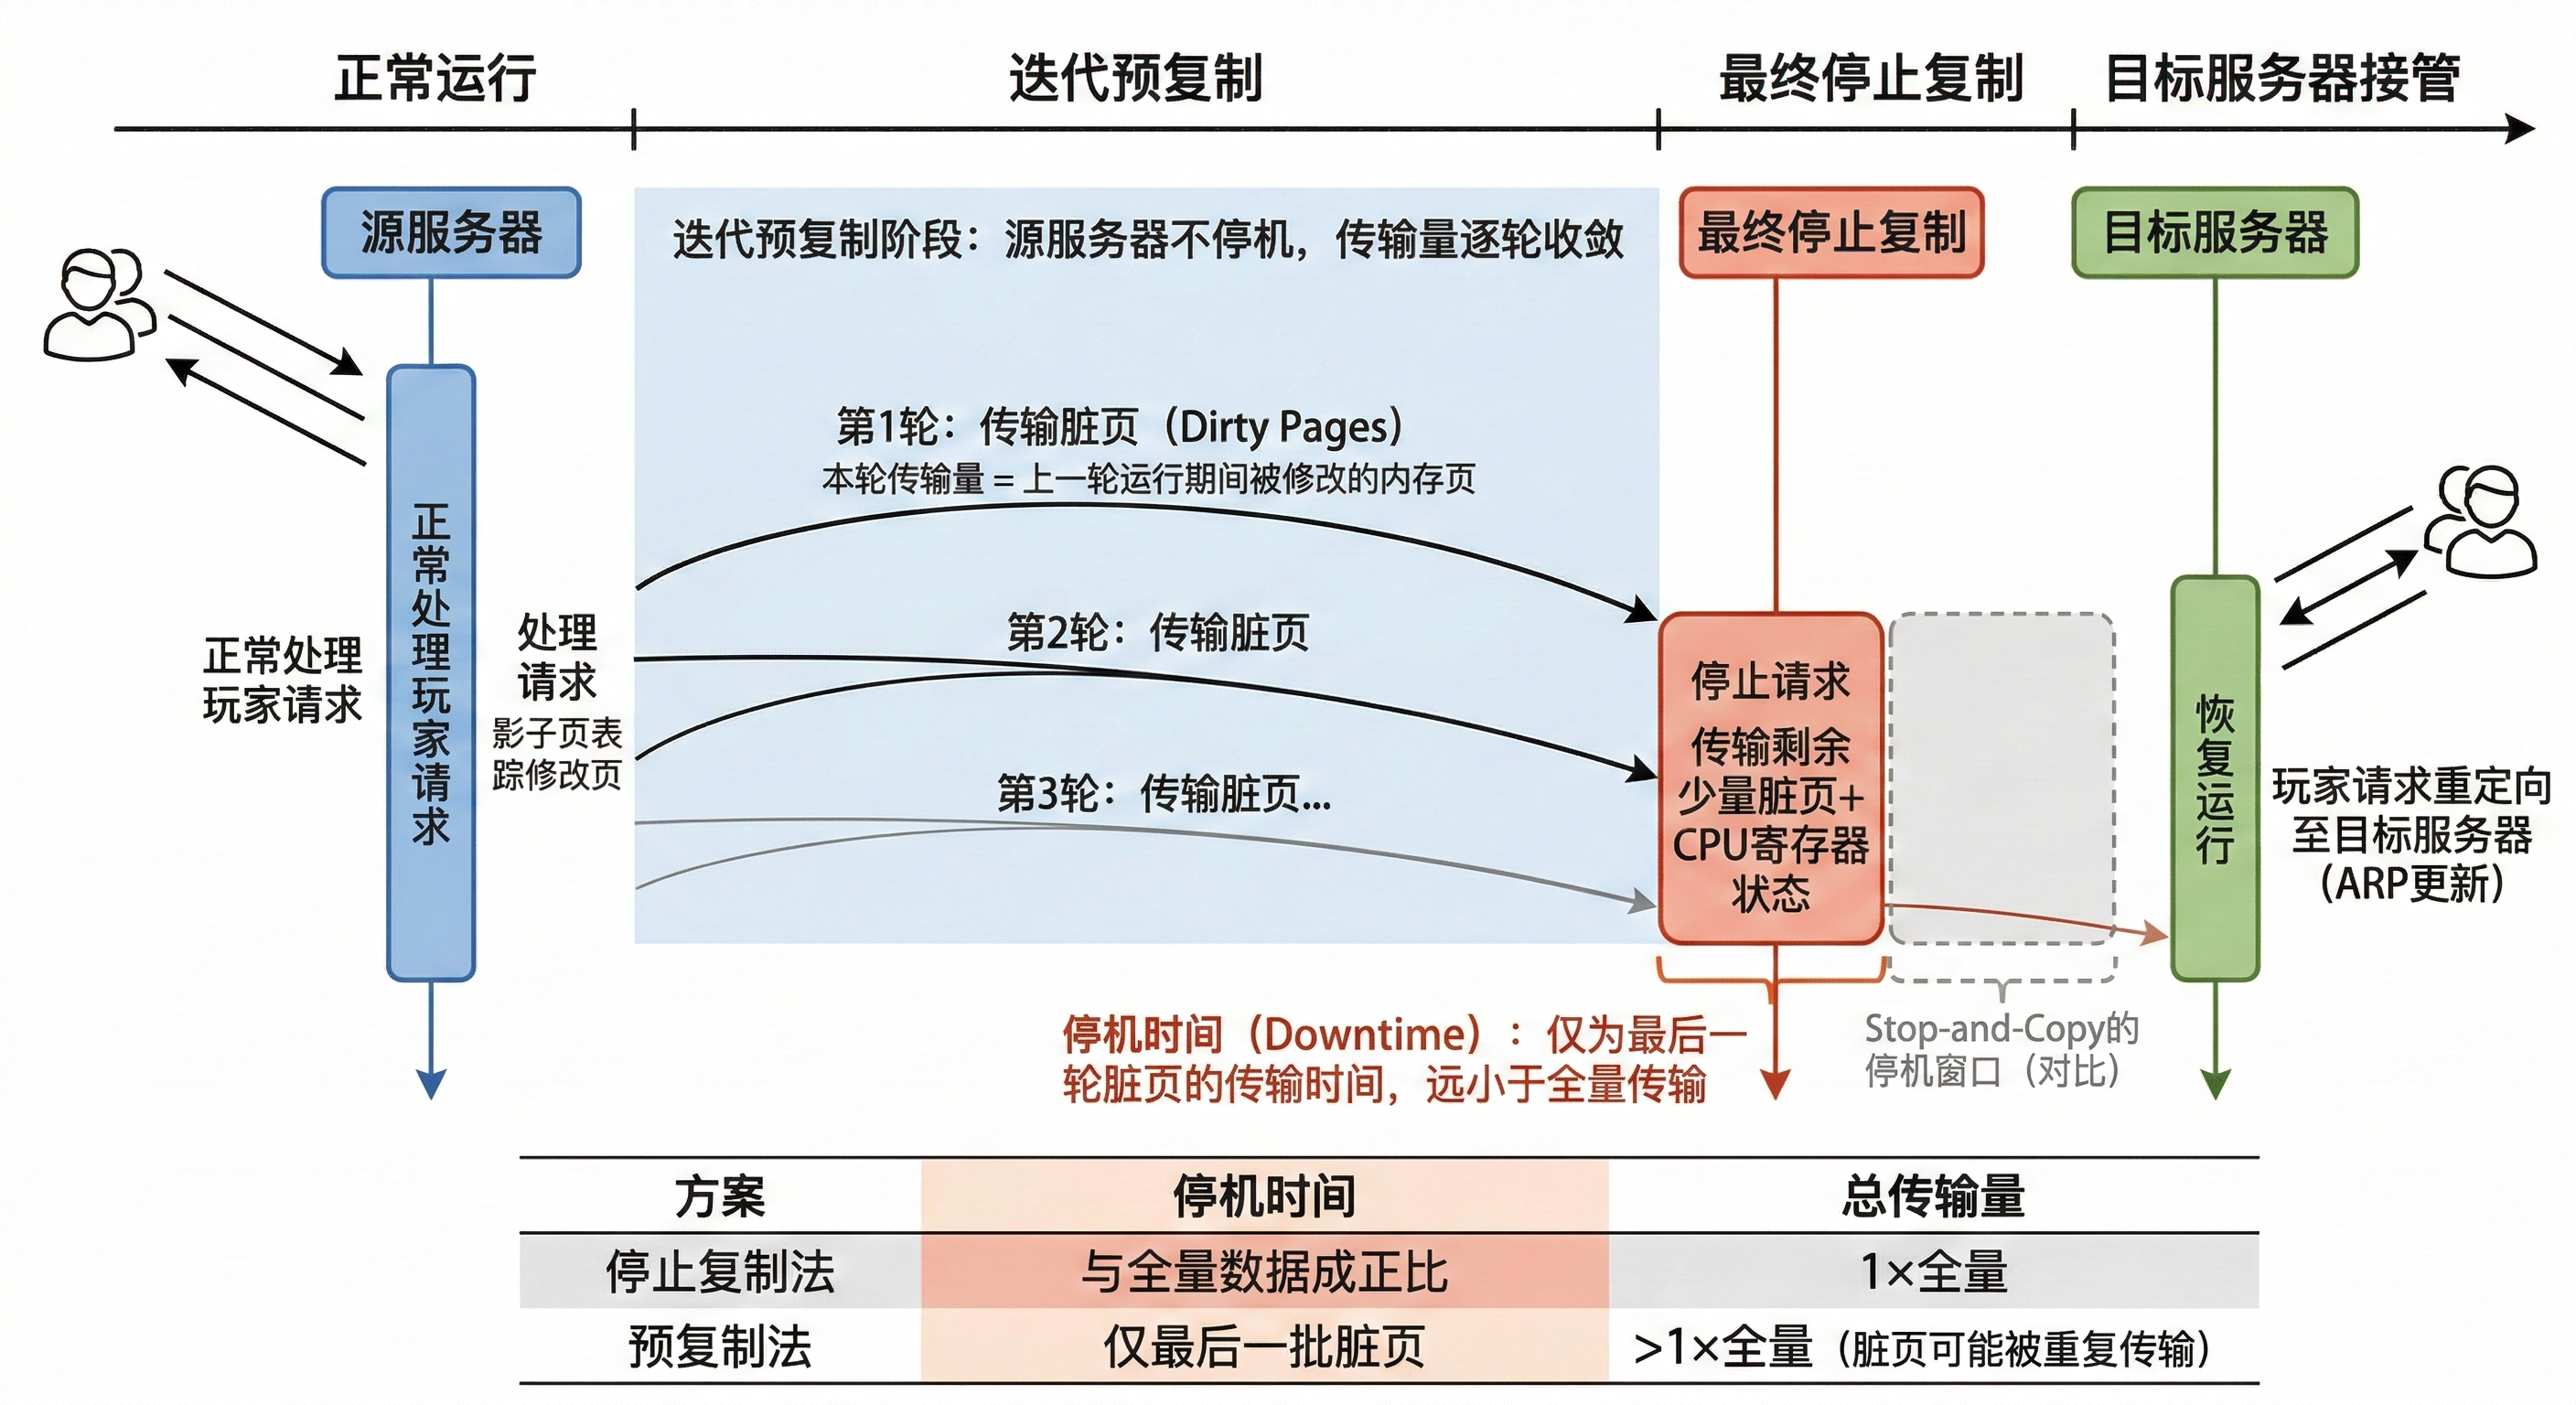
\includegraphics[width=1\linewidth]{figures/sec4/4-migrate-precopy.png}
    \caption{预复制法（Pre-Copy）：源服务器持续运行，迭代传输脏页直至收敛，
    最终仅需极短停机传输剩余脏页；停机时间远小于停止复制法，但总传输量更大}
    \label{fig:migration_precopy}
\end{figure}

\paragraph{方案三：按优先级分波迁移（Wave-Based Migration）}

停止复制法和预复制法都来源于虚拟机迁移领域，将玩家所在的整个服务器进程视为迁移单元，
迁移的是完整的内存镜像。但对于游戏服务器来说，并不是所有内存状态对玩家的即时体验
都同等重要——在玩家切换服务器的那一帧，最关键的只是角色位置、动画帧、生命值这几项数据；
场景中视野外的敌人状态、已完成战斗的历史记录，晚几百毫秒同步完全没有问题。
这一洞察催生了面向游戏场景的分波迁移法（Wave-Based Migration），
如图~\ref{fig:migration_wave} 所示。

分波迁移的流程分为三个阶段。第一步是预热阶段：在迁移实际发生之前，
目标服务器提前收到指令，加载该玩家所在关卡的静态资源（地图、关卡配置、
通用对象列表），这一步可以在玩家完全无感知的情况下在后台完成，
将原本需要数秒的资源加载时间从关键路径上彻底移除。
第二步是触发与第一波同步：当迁移正式触发时，
源服务器向目标服务器发送第一波状态——仅包含对即时玩家体验至关重要的少量数据：
玩家角色的当前位置与朝向、精确到帧的动画状态、当前血量与技能冷却。
由于第一波数据极小（通常在数 KB 以内），目标服务器几乎立刻就能据此渲染出
对玩家而言视觉连续的第一帧画面并发回客户端，使得玩家感知到的服务中断时间
压缩至不足 25 毫秒——在 30 帧/秒的游戏中，这甚至不到一帧的时间。
第三步是后续波次的静默同步：在客户端已经恢复正常接收帧的同时，
源服务器继续将视野范围内的其他对象状态（第二波）、视野外的全局对象状态（第三波）
逐步传输给目标服务器，目标服务器在后台完成这些数据的恢复，整个过程对玩家完全透明。

\begin{tcolorbox}[title=按优先级分波迁移的核心逻辑]
\begin{lstlisting}[
    language=go,
    basicstyle=\ttfamily\footnotesize,
    aboveskip=0pt, belowskip=0pt,
    lineskip=-1pt,
    commentstyle=\color{gray},
    keywordstyle=\color{blue}\bfseries,
    breaklines=true
]
// 阶段0：提前预热目标服务器（后台静默执行）
targetServer.PreloadStaticAssets(player.CurrentLevel)

// 触发迁移：发送触发信号，源服务器发出最后一帧
triggerMigration(sourceServer, targetServer, player)

// 第一波：最小关键状态（毫秒级，决定玩家感知的中断时长）
wave1 := PlayerCriticalState{
    Position:      player.Position,
    AnimatorFrame: player.AnimatorFrame,  // 精确到帧，保证动画连续
    HP:            player.HP,
    CameraState:   player.Camera,
}
targetServer.ApplyWave(1, wave1)
// 目标服务器立即渲染第一帧并发回客户端，服务恢复

// 第二波：视野内其他对象（后台同步，玩家已恢复正常游戏）
wave2 := collectVisibleObjects(player)
targetServer.ApplyWave(2, wave2)

// 第三波：视野外全局对象（后台静默，完全无感）
wave3 := collectAllRemainingObjects(player)
targetServer.ApplyWave(3, wave3)

// 源服务器确认迁移完成，清理该玩家的会话和内存
sourceServer.CleanupPlayer(player)
\end{lstlisting}
\end{tcolorbox}

\begin{figure}[htbp]
    \centering
    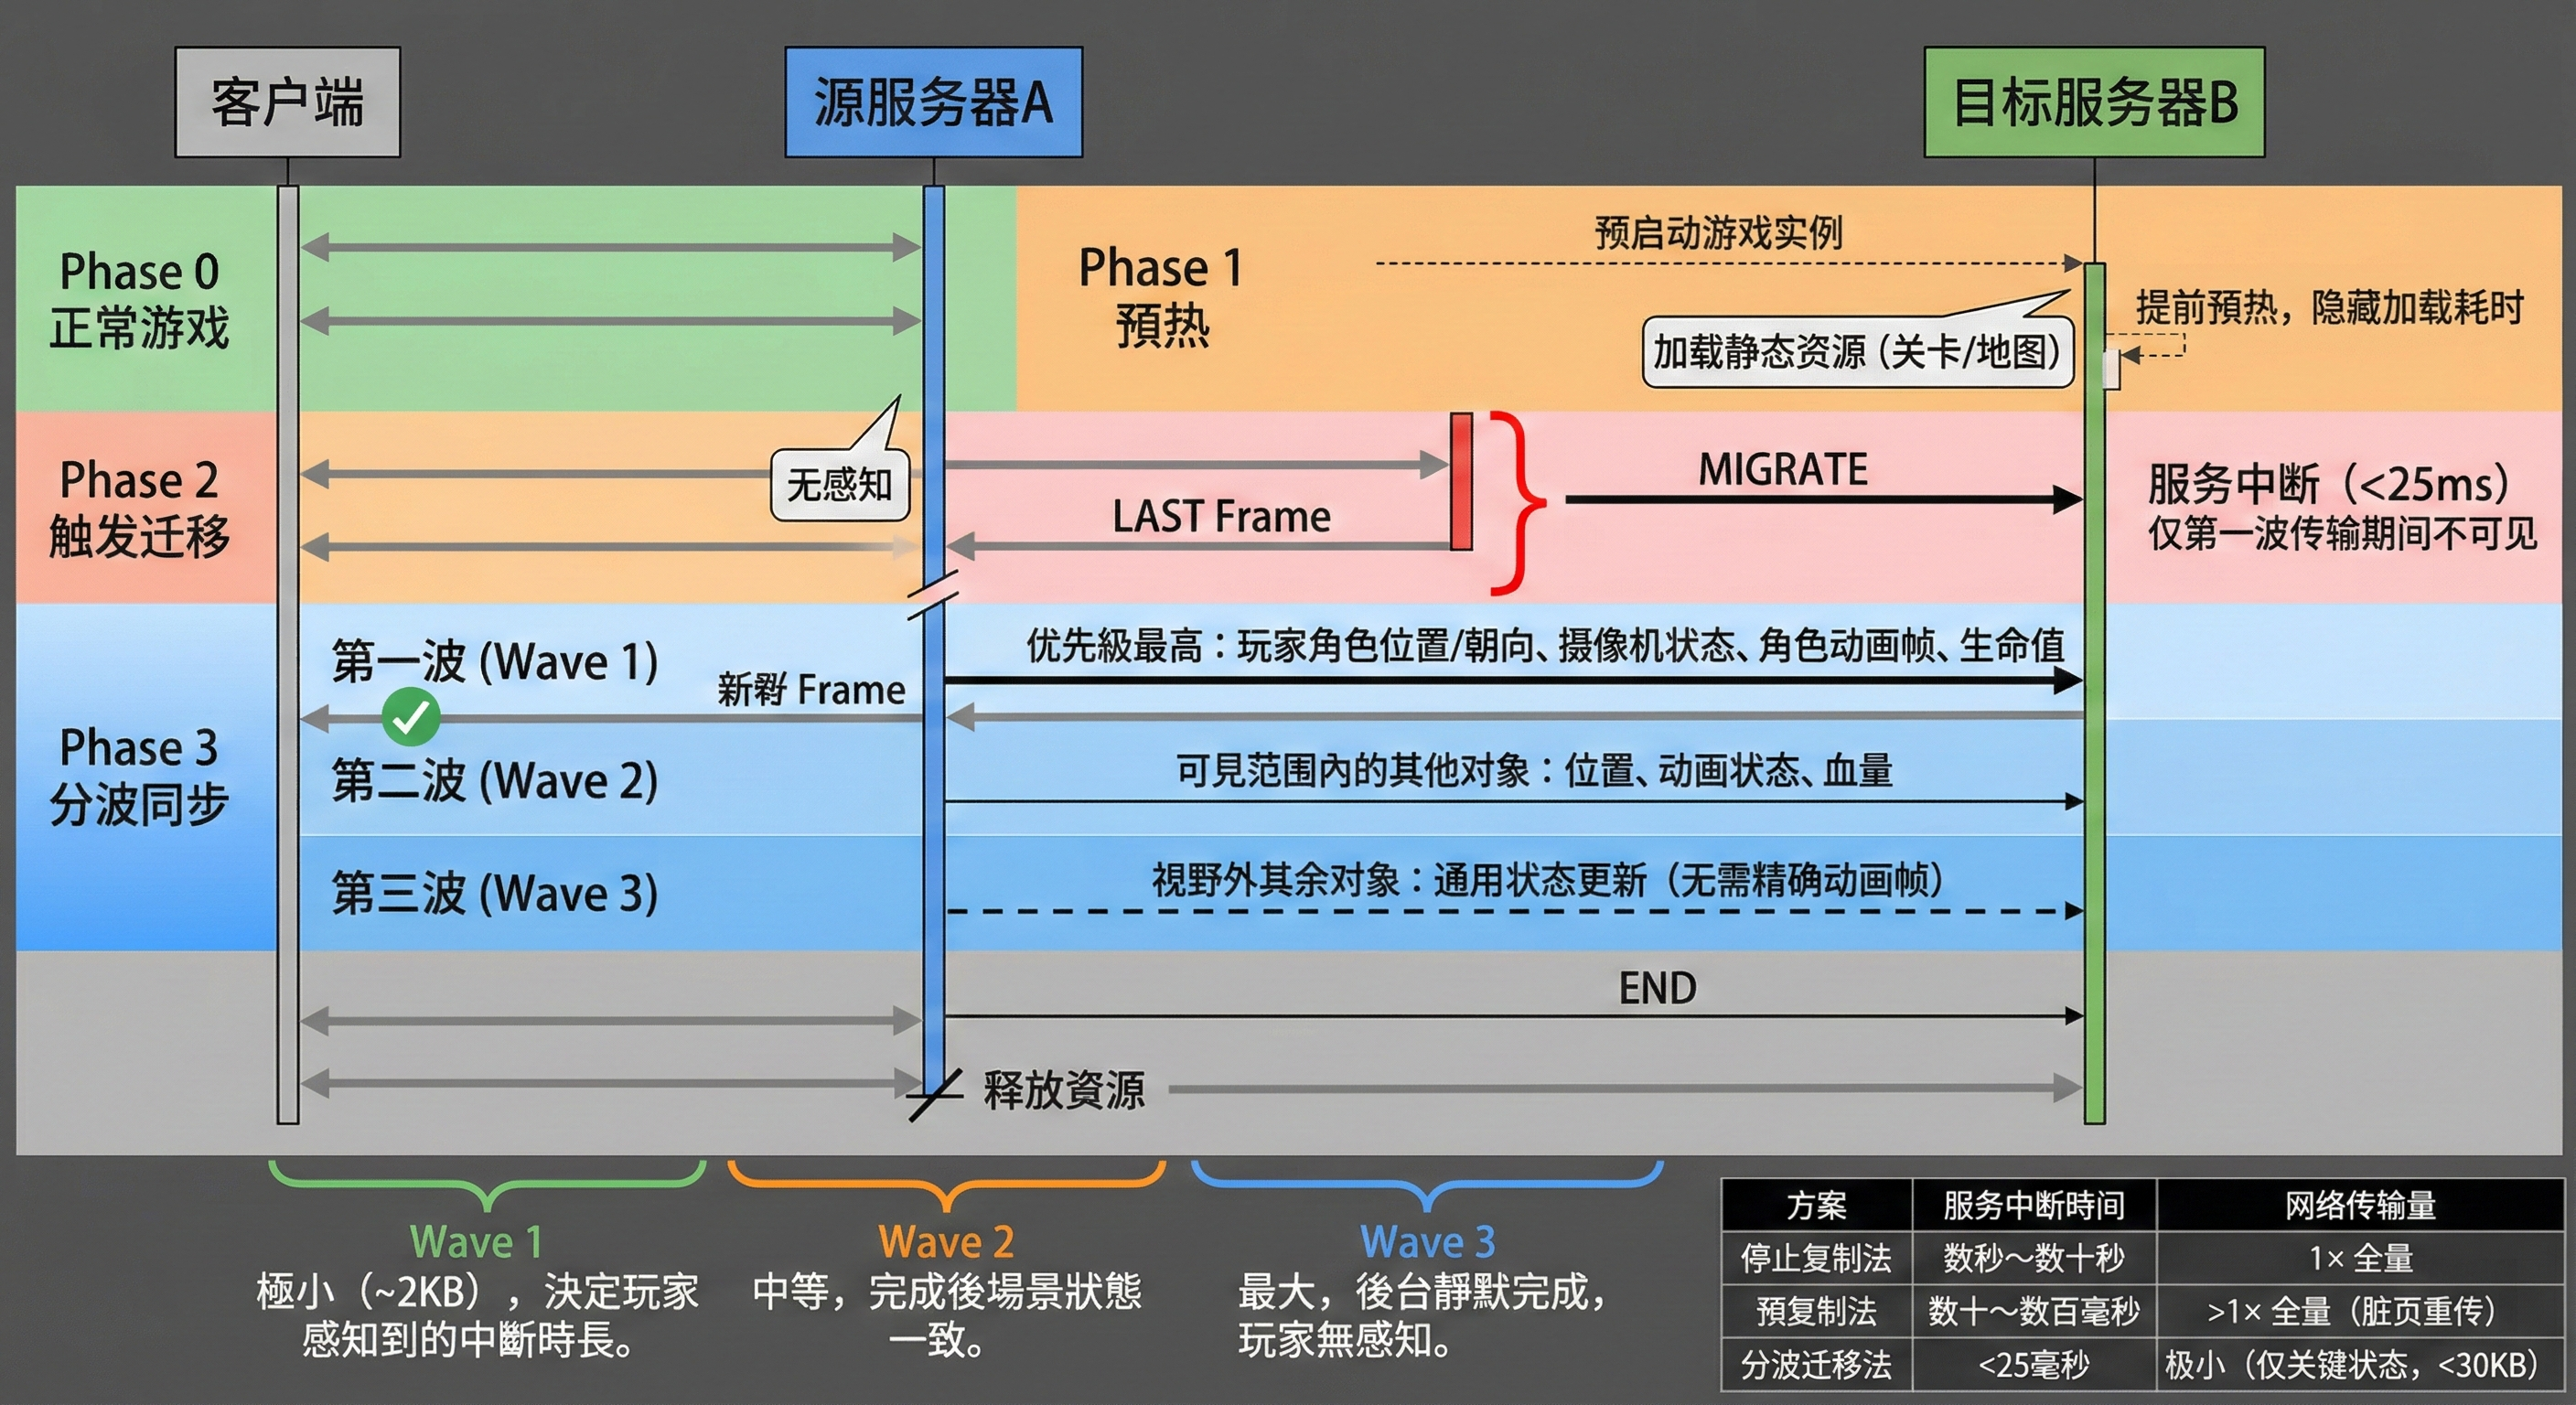
\includegraphics[width=1\linewidth]{figures/sec4/4-migrate-wave.png}
    \caption{按优先级分波迁移：第一波仅传输角色位置、动画帧等极少量关键数据（<30KB），
    使玩家服务中断低于 25ms；后续波次在客户端已恢复正常后于后台静默完成，
    总传输量远小于全量内存复制}
    \label{fig:migration_wave}
\end{figure}

三种方案的本质区别在于如何权衡停机时间、传输量和实现复杂度。
停止复制法以最简单的实现换来最长的停机时间，适合维护窗口或离线场景。
预复制法通过迭代传输脏页大幅压缩停机时间，但总传输量更大，
适合通用服务器迁移场景，VMware 的 vMotion 和 Xen 的虚拟机热迁移均采用此思路。
分波迁移法则针对游戏场景的领域特性——状态有明确的重要性层次——
将停机时间压缩到单帧以内，代价是需要开发者在引擎层面对游戏状态进行优先级分类，
实现复杂度最高，但玩家体验最佳。

无论采用哪种迁移方案，在工程实践中都需要配合两项约束来防止迁移本身成为新的负担。
其一是迁移冷却期：同一台服务器在执行一次迁移后需要等待一段时间（如 30 分钟）
才能再次触发，避免迁移操作频繁进行，给服务器间网络带宽带来持续压力。
其二是单次迁移的玩家数量上限：每次迁移不宜超过一定规模（如 100 人），
防止目标服务器因短时间内涌入大量新会话而出现新的过载，
使得原本的缓解措施反而制造了新的热点。



\subsection{跨服擂台：分布式环境下的玩家交互}

当数据被拆分、负载被均衡之后，游戏世界从"一台大服务器"演化成了"许多协同工作的服务器"：不同机器上运行着不同的游戏区服，每一台都在忙碌地照看自己负责的那一片玩家群体。在这样的世界里，一个自然的想法会浮现出来：既然玩家已经被分散到多个服务器上，能不能让他们在某一个玩法里"跨服相遇"？

这个想法并非凭空而来，而是源于分布式架构本身带来的一个副作用。当我们为了承载更多玩家而将他们分散到多台服务器时，无意中也在玩家群体之间竖起了一道道无形的墙——服务器 1 的玩家只能看到服务器 1 的其他玩家，服务器 2 的玩家只能看到服务器 2 的其他玩家，彼此之间完全隔离，就像生活在平行宇宙中。对于一些需要大量玩家参与的玩法（比如公会战、世界 BOSS），这种隔离问题不大；但对于竞技性的 PvP 玩法，这种隔离会带来一些负面影响：人少的服务器玩家找不到对手，人多的服务器玩家总是遇到同样的老面孔，新鲜感和竞技性都会下降。

跨服擂台，正是这样一种试图打破服务器壁垒、把分布式架构转化为玩法优势的尝试。它的核心理念是：虽然玩家的数据分散存储在不同的数据库分片上，虽然玩家平时连接的是不同的游戏服务器，但在"擂台"这个特定的玩法场景中，我们可以让所有服务器的玩家汇聚到一个统一的竞技平台上，在这里他们可以看到来自全区全服的对手，可以挑战任何一个报名参赛的玩家，不再受服务器边界的限制。本节将通过这个跨服擂台案例，展示分布式环境下如何实现玩家交互、如何保证全局一致性，以及如何设计一个可靠的协调机制。

\subsubsection{跨服交互的设计思路与核心挑战}

在传统的单服架构中，玩家只能与同一台服务器上的其他玩家互动。这种限制在一定程度上保证了系统的简单性——所有相关的数据都在同一个数据库中，所有相关的计算都在同一台服务器上，不需要考虑跨机器通信、数据同步、一致性保证这些复杂问题。但它也带来了一个显而易见的弊端：服务器之间的玩家群体是割裂的。

这种割裂在不同规模的服务器上会产生不同的问题。对于玩家数量较少的服务器——可能是新开的服务器，也可能是老服务器上的玩家逐渐流失——活跃玩家之间很快就会互相熟悉，每天匹配到的对手总是那么几个人。久而久之，玩家会感到竞技的新鲜感在下降，因为对手的打法、战力、习惯都已经了如指掌，缺少了探索和未知的乐趣。更严重的是，当活跃玩家数量低于某个阈值时，匹配系统可能需要很长时间才能找到一个合适的对手，甚至完全匹配不到人，玩家只能放弃这个玩法。对于玩家数量众多的服务器，虽然不存在"找不到人"的问题，但也有另一种困扰：人多的服务器往往竞争更激烈，想要在排行榜上占据靠前的位置，需要投入大量的时间和精力，甚至需要氪金强化装备。而在人少的服务器上，同样的战力可能轻松登顶。这种服务器之间的难度差异，会让玩家产生"选错服务器"的遗憾感。

跨服擂台的设计初衷，就是打破这种服务器之间的壁垒，让来自不同服务器的玩家能够在一个统一的竞技平台上相遇、较量。从玩家的角度看，这意味着潜在的对手池从"本服的几百人"扩大到了"全区全服的几万人甚至几十万人"，匹配速度更快，对手更多样化，竞技性更强。从运营的角度看，跨服玩法可以缓解不同服务器之间玩家活跃度差异带来的问题，让所有玩家都能享受到足够的游戏乐趣，减少因"服务器人太少"而导致的玩家流失。

但要在分布式环境下实现跨服交互，技术复杂度会显著提升。在单服环境中，当两个玩家进行战斗时，他们的状态数据都在同一个服务器的内存中，战斗逻辑可以直接读取双方的属性、技能、装备，模拟战斗过程，计算伤害和血量变化，最后给出胜负结果，整个过程都是本地的、同步的、确定的。但在跨服环境中，挑战者可能在服务器 1，被挑战者可能在服务器 2，他们的状态数据分别存储在两个不同的数据库分片中。这就带来了一系列问题：战斗逻辑该在哪里执行？是在服务器 1、服务器 2，还是需要一个第三方的"战斗服务器"？如果战斗结果在服务器 1 上计算出来，如何确保服务器 2 也能及时、准确地获取这个结果，并更新本地玩家的数据？如果网络出现延迟或中断，导致两台服务器对同一场战斗的结果产生了分歧，又该如何处理？

为了在有限的篇幅内清晰地讲解跨服交互的核心概念，而不被过多的实现细节淹没，我们在设计跨服擂台时做了一个重要的简化：刻意弱化空间维度，只保留最核心的一条规则——每位玩家有一个战力值，当玩家在擂台中挑战他人时，系统只需要根据双方战力的大小关系给出胜负结果。在这个模式里，没有位置信息、没有移动轨迹、没有碰撞检测、没有技能释放、没有实时的帧同步，整个玩法更像是一场静态的"战力比拼"——比的不是操作技巧或战术策略，而是角色的培养程度和装备强度。这种简化让我们可以把注意力集中在分布式系统的核心问题上：如何在多台独立的服务器之间协调状态、如何保证全局的一致性、如何设计一个可靠的裁决机制。这些问题在任何跨服玩法中都会遇到，无论是简单的战力比拼，还是复杂的实时对战。

\subsubsection{架构设计：协调服务器与代理模式}

从玩家的视角看，跨服擂台的使用流程是这样的：无论玩家身处哪个服务器，只要等级或条件满足，便可以在本服的界面上打开"擂台入口"。入口中会列出当前所有已经报名的擂台玩家，他们来自不同的大区和服务器，每个人的条目上标记着名字、战力值以及所属服务器。玩家可以从列表中选择一个对手发起挑战，系统片刻之后返回战斗结果——比如"恭喜你战胜了来自华北三区的剑客李四！"整个流程在玩家看来是连贯而自然的，但在服务器背后，却涉及多个独立系统之间的协同工作。

把玩家的体验流程翻译回服务器世界，可以得到这样一幅架构图景：在众多游戏服务器之外，需要部署一个专门负责擂台逻辑的"擂台协调服务器"。这个协调服务器是整个跨服擂台系统的核心，它既不承载普通的游戏地图，也不处理玩家的移动和战斗，而是专注于三个职责：第一，维护一份全局的擂台报名列表，记录所有参与擂台的玩家信息（包括玩家 ID、昵称、战力值、所属服务器、当前状态等）；第二，在有人发起挑战时根据双方战力值给出裁决，判定胜负；第三，将战斗结果以事件的形式分发给相关的游戏服务器，通知它们更新本地数据。

各个游戏服务器在这个架构中扮演的是"擂台代理"的角色。一方面，它们负责把本服想要报名的玩家信息发送到擂台协调服务器，相当于在全局的擂台名单中"登记"一个条目；另一方面，当本服玩家想要查看对手列表或发起挑战时，游戏服务器会将请求转发给擂台协调服务器，等待协调服务器返回结果，再把结果呈现给玩家；最后，当战斗结束、协调服务器返回战斗结果时，游戏服务器负责把这些变化融入本地的任务系统、奖励系统和界面表现之中——比如增加玩家的擂台积分、更新擂台排名、发放胜利奖励、推送战斗通知等。

\begin{figure}[htbp]
    \centering
    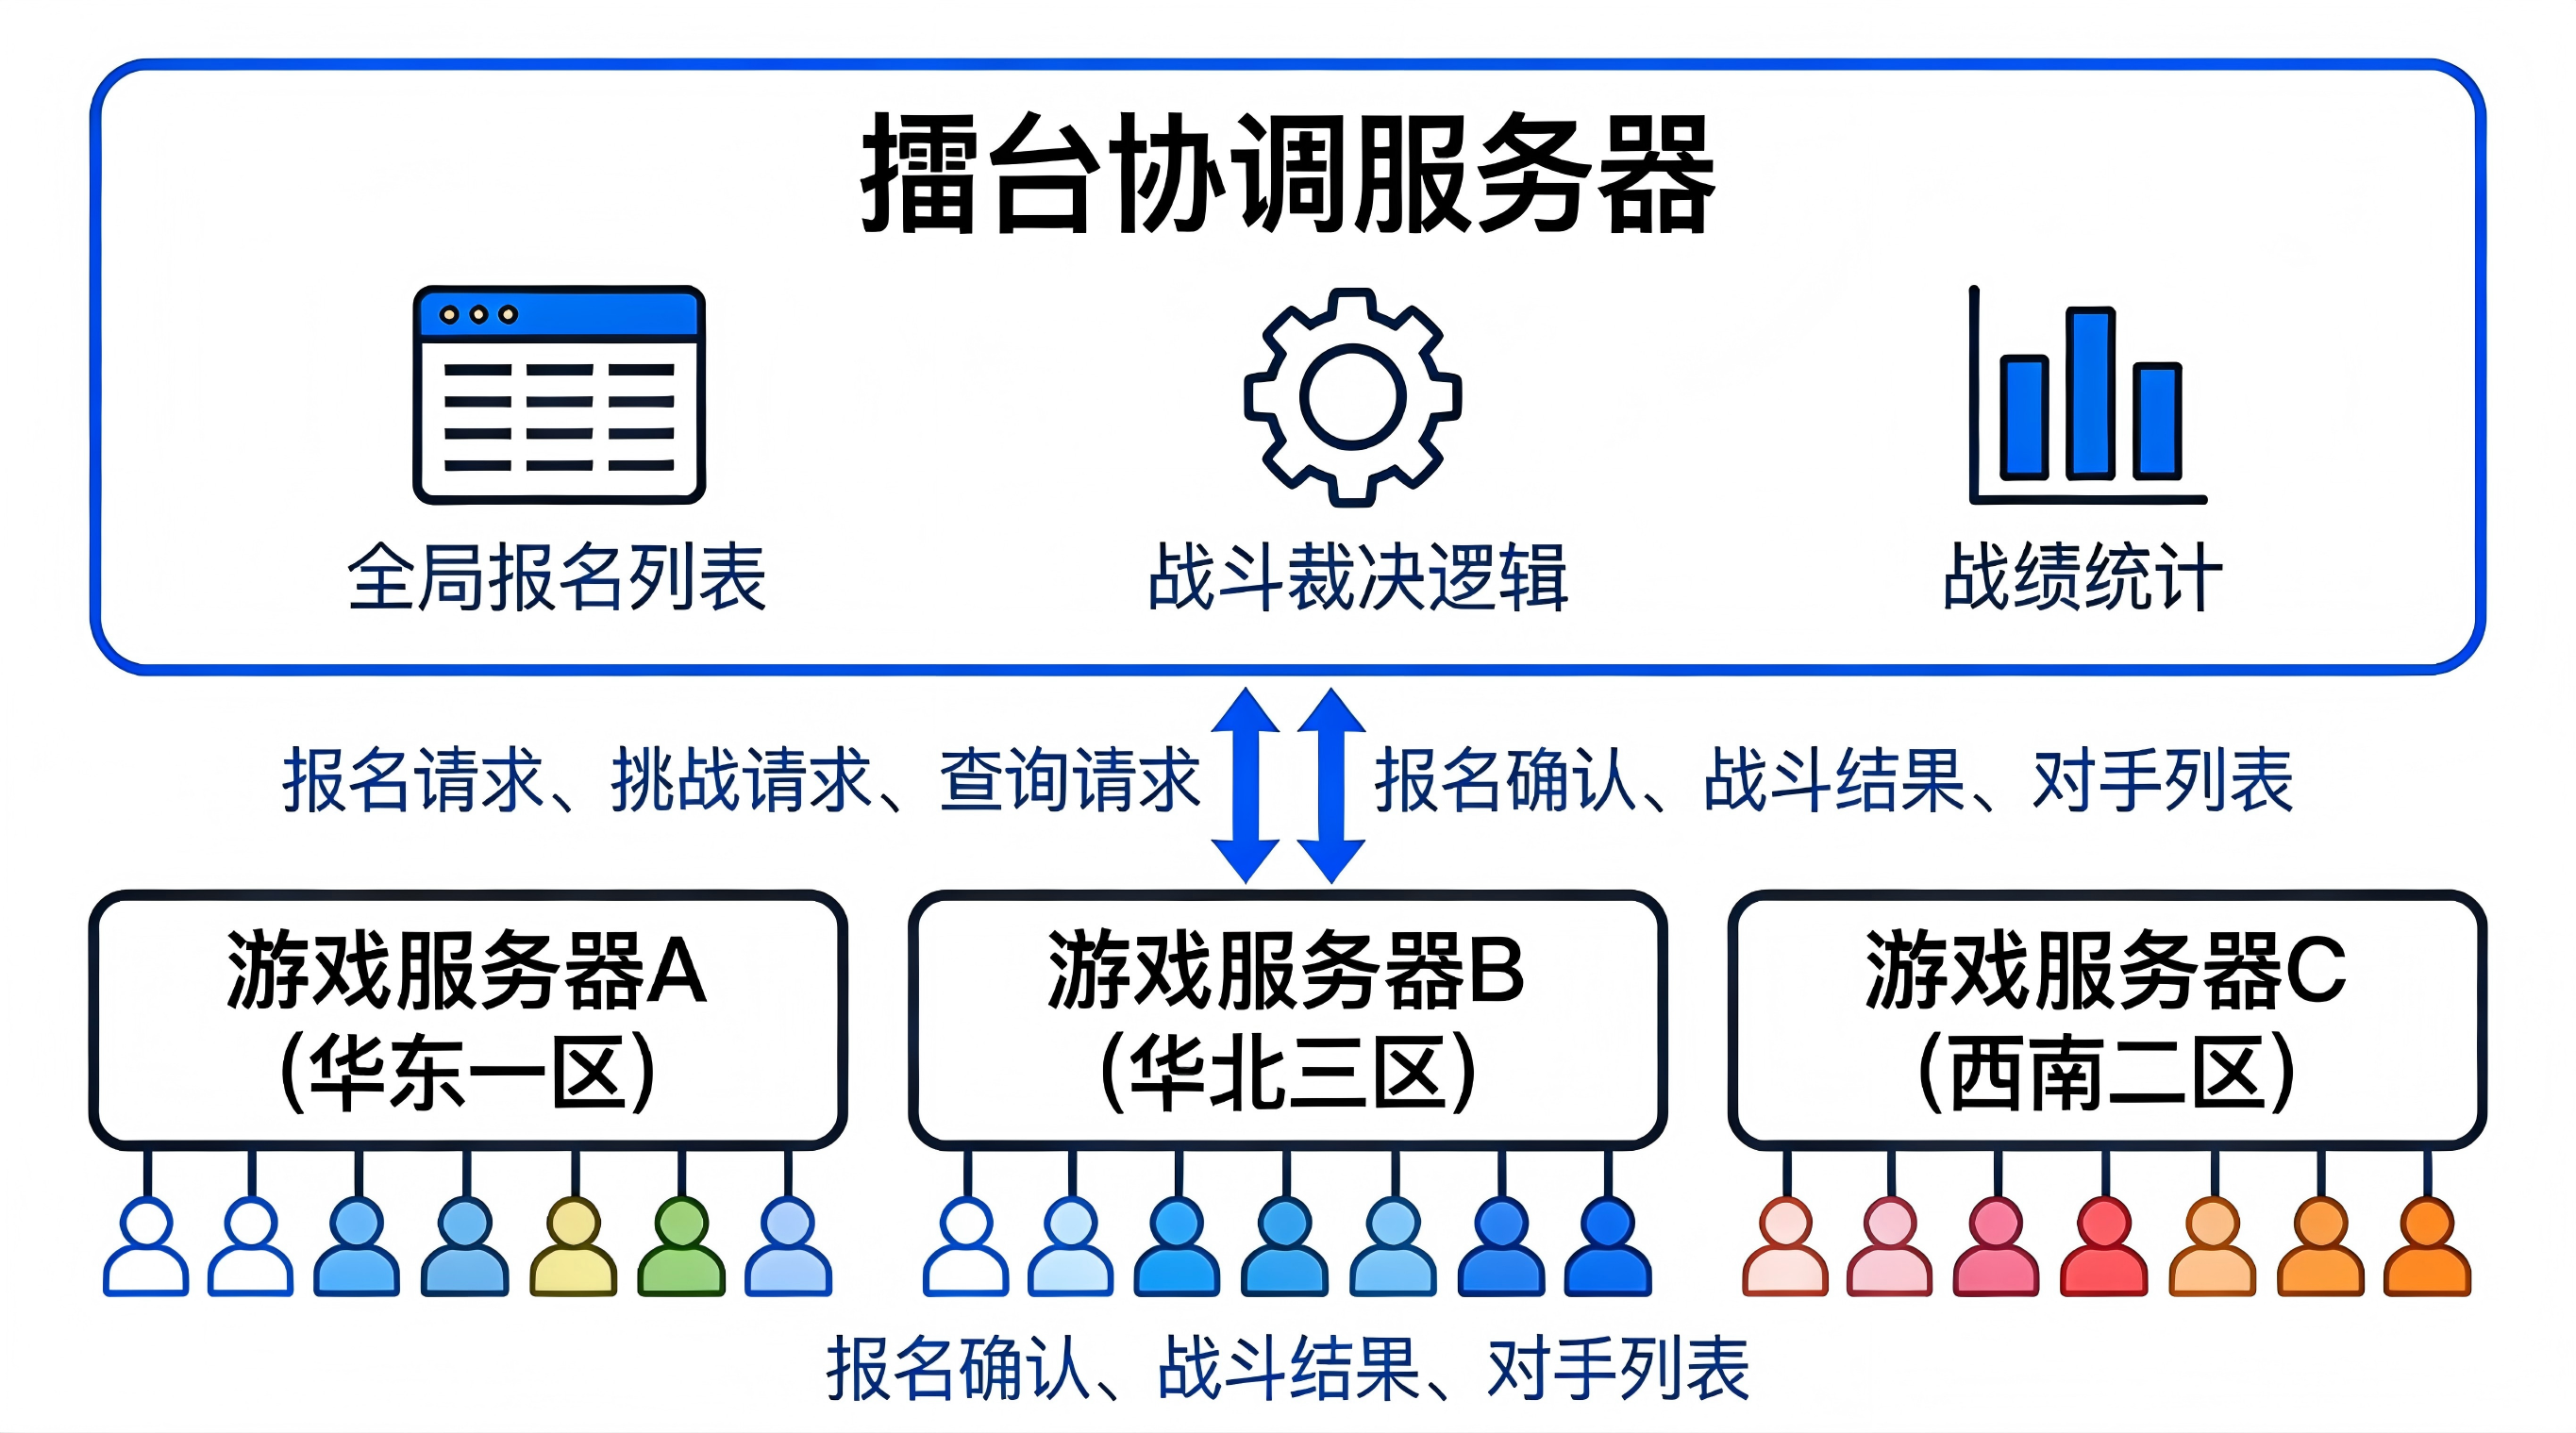
\includegraphics[width=1\linewidth]{figures/sec4/4-4.png}
    % 图片描述：跨服擂台的架构示意图
    % 顶部：一个大的矩形框，标注"擂台协调服务器"，内部包含：
    %   - "全局报名列表"（表格图标）
    %   - "战斗裁决逻辑"（齿轮图标）
    %   - "战绩统计"（柱状图图标）
    % 底部：三个游戏服务器并排，分别标注"游戏服务器A（华东一区）"、"游戏服务器B（华北三区）"、"游戏服务器C（西南二区）"
    % 每个游戏服务器下方连接若干玩家图标
    % 游戏服务器与擂台协调服务器之间有双向箭头，标注：
    %   - 上行箭头："报名请求、挑战请求、查询请求"
    %   - 下行箭头："报名确认、战斗结果、对手列表"
    % 用不同颜色区分不同服务器的玩家
    % 所有文字使用简体中文
    \caption{跨服擂台的整体架构}
    \label{fig:cross_server_arena_architecture}
\end{figure}

在这种架构下，擂台协调服务器承担了一个跨服视角下的"统一真相源"角色。它知道有哪些玩家正在参与擂台——无论这些玩家来自哪个服务器、数据存储在哪个分片——他们各自的战力是多少、目前是否在战斗之中、已经打了多少场、胜率如何。这一层信息在逻辑上属于全局，没有哪个单独的游戏服务器可以声称"我拥有全部擂台的信息"。即使是人数最多的服务器，也只知道本服玩家的情况，对其他服务器的玩家一无所知。而各个游戏服务器则负责把这一全局真相以本服玩家能够理解和感知的方式呈现出来：在界面上以列表展示所有参赛玩家，在本地记录本服玩家的胜负场次、更新积分和排名、发放奖励。从数据流的角度看，擂台协调服务器是"上游"，负责维护全局状态和做出权威裁决；各个游戏服务器是"下游"，负责接收上游的指令并在本地执行。这种单向的数据流和清晰的职责划分，是保证跨服系统正确运行的关键。

\subsubsection{报名与查询：全局状态的构建}

现在我们逐一分析跨服擂台的几个核心流程。首先是报名流程。当玩家小明在"华东一区"的游戏服务器上点击"报名参赛"按钮时，客户端会向游戏服务器发送一条报名请求消息。游戏服务器收到这条消息后，首先会执行一系列本地的前置检查：玩家等级是否达到参赛要求（比如至少 30 级）？玩家当前是否处于其他战斗中？玩家是否已经在擂台中报名？玩家今天是否还有剩余的报名次数？玩家的战力值是否已正确计算？这些检查的目的是在数据离开本服之前，就把明显不合法的请求过滤掉，减轻协调服务器的压力，也能更快地给玩家反馈。

如果所有检查都通过，游戏服务器会提取玩家的关键信息，构造一条报名请求，发送给擂台协调服务器。这条请求中包含玩家 ID、昵称、战力值、所属服务器 ID、报名时间戳等信息。擂台协调服务器收到报名请求后，也会执行一系列检查：检查这个玩家 ID 是否已经在全局的报名列表中（注意这里检查的是全局列表，即使玩家之前在另一台游戏服务器上报名，也能被检测到）；检查擂台当前是否已达到人数上限（为了保证系统性能和用户体验，擂台可能会设置一个参赛人数上限，比如最多 10 万人）；检查擂台当前是否处于开放时间（有些擂台玩法会设置固定的开放时间，比如每周六 14:00-16:00）；检查擂台是否正在维护。

\begin{tcolorbox}[title=报名请求的处理流程]
\begin{lstlisting}[
    language=go,
    basicstyle=\ttfamily\footnotesize,
    aboveskip=0pt, belowskip=0pt,
    lineskip=-1pt,
    commentstyle=\color{gray},
    keywordstyle=\color{blue}\bfseries,
    breaklines=true
]
// 游戏服务器：本地检查 -> 构造请求
if player.Level < 30 {
    return "等级不足，需要30级"
}
req = {PlayerID, Nickname, PowerValue, ServerID, Timestamp}
resp = arenaCoordinator.Register(req)

// 协调服务器：全局检查 -> 添加到列表
if alreadyExists(req.PlayerID) {
    return "已经报名"
}
addToGlobalList(req)
return {Success: true, TotalPlayers: len(globalList)}
\end{lstlisting}
\end{tcolorbox}

如果一切正常，协调服务器会将玩家信息添加到全局的报名列表中，并返回报名成功的响应。响应中包含当前的总参赛人数，游戏服务器收到后会在界面上显示"报名成功！当前全区共有 8327 名玩家参赛"，给玩家一个直观的反馈——这个数字不仅仅是本服的参赛人数，而是所有服务器加起来的总数，这正是跨服玩法的魅力所在。

报名成功后，玩家需要看到当前有哪些对手可以挑战。最直接的做法是，游戏服务器向擂台协调服务器发起一个查询请求："给我当前所有已报名且未在战斗中的玩家列表。"协调服务器遍历全局的报名列表，筛选出符合条件的玩家，将完整的列表返回给游戏服务器。但这种做法在擂台人数较多时会遇到性能问题。假设有 10 万玩家报名，每个玩家的信息包含 ID、昵称、战力值、服务器 ID 等字段，平均每条记录 100 字节，完整的列表就是 10MB 的数据。如果同时有 1000 个玩家在查询对手列表，协调服务器需要在短时间内发送 10GB 的数据，这对网络带宽和服务器 CPU 都是巨大的压力。更严重的是，这 10 万条记录中，大部分玩家对于当前请求的玩家来说都是"不相关"的——比如战力相差太大的玩家，挑战胜算很小或根本没有挑战价值。

因此，实际系统中通常会采用分页查询和条件筛选的方式。玩家不是一次性拿到所有对手的列表，而是先拿到一小部分（比如 50 个），在界面上滚动浏览时再加载更多。同时，查询请求中可以携带筛选条件，比如"只返回战力在我 ±5000 范围内的对手"、"只返回胜率低于 60\% 的对手"、"优先返回与我同服务器的对手"等，大大减少返回的数据量。协调服务器在收到查询请求后，会先根据筛选条件过滤出符合要求的玩家，再按战力值或其他维度排序，最后截取指定页码的数据返回。这样每次请求返回的数据量可以控制在一个合理的范围内（比如 50 条记录约 5KB），即使有数万玩家同时查询，协调服务器也能稳定应对。

\subsubsection{挑战与裁决：唯一真相源的必要性}

当玩家从对手列表中选择一个目标并点击"挑战"按钮时，整个系统进入了最核心的环节：战斗裁决。游戏服务器会构造一条挑战请求，包含挑战者的玩家 ID 和被挑战者的玩家 ID，发送给擂台协调服务器。协调服务器收到挑战请求后，首先要做一系列的合法性检查，这是保证系统正确性和公平性的关键：挑战者和被挑战者是否都在报名列表中（有可能某个玩家刚刚取消报名或被系统移除，但客户端界面还没刷新）？挑战者和被挑战者是否都处于"空闲"状态（如果其中任何一方正在进行其他战斗，不允许开始新的战斗，避免一个玩家同时参与多场战斗导致状态混乱）？挑战者今天的挑战次数是否已用完？挑战者是否在冷却时间内？

如果所有检查都通过，协调服务器会将双方的状态标记为"战斗中"，防止在战斗结束之前被其他玩家同时挑战。想象一下，如果玩家 A 正在与玩家 B 战斗，此时玩家 C 也向 B 发起挑战，那 B 应该同时与 A 和 C 战斗吗？显然不合理。通过状态锁定机制，我们确保同一时刻一个玩家只能参与一场战斗。

接下来是战斗裁决的核心逻辑。在我们简化的跨服擂台中，战斗规则非常简单：比较双方的战力值，战力值更高的一方获胜。如果战力值相等，可以引入随机因素或其他平局打破器（比如等级、装备品质）。协调服务器执行裁决后，会生成一个战斗结果事件，记录胜者和败者，并更新双方的擂台战绩——比如胜者的胜场数加一，败者的负场数加一。战斗结算完成后，协调服务器会将双方的战斗状态恢复为"非战斗中"，并将战斗结果事件分别发送给挑战者和被挑战者所属的游戏服务器。

\begin{tcolorbox}[title=战斗裁决的核心流程]
\begin{lstlisting}[
    language=go,
    basicstyle=\ttfamily\footnotesize,
    aboveskip=0pt, belowskip=0pt,
    lineskip=-1pt,
    commentstyle=\color{gray},
    keywordstyle=\color{blue}\bfseries,
    breaklines=true
]
// 1. 锁定双方状态
challenger.Status = "fighting"
defender.Status = "fighting"

// 2. 战斗裁决（简化规则：战力高者胜）
if challenger.Power > defender.Power {
    winner = challenger
} else {
    winner = defender
}

// 3. 更新战绩并解锁状态
winner.Wins++, loser.Losses++
challenger.Status = "idle", defender.Status = "idle"

// 4. 分发结果到双方服务器
sendResult(challengerServer, result)
sendResult(defenderServer, result)
\end{lstlisting}
\end{tcolorbox}

注意这里是"分别发送"——挑战者可能在服务器 A，被挑战者可能在服务器 B，协调服务器需要向两台不同的服务器各发送一条消息，通知它们战斗的结果。各个游戏服务器收到战斗结果事件后，需要根据事件中的信息更新本地玩家的数据。如果本服玩家是胜者，游戏服务器会增加玩家的擂台积分、发放胜利奖励（比如金币、擂台代币）、更新任务进度（比如"赢得 10 场擂台战斗"）；如果本服玩家是败者，则可能扣除一些积分或记录失败次数。这些更新操作完全在本地进行，不需要再与擂台协调服务器或其他服务器通信，从而避免了复杂的分布式事务。

需要强调的是，各个游戏服务器在收到战斗结果事件后，并不会对结果本身进行任何质疑或修改。它们只是忠实地执行擂台协调服务器给出的裁决，将结果体现在本地数据和界面表现中。即使某个游戏服务器的本地数据显示玩家的战力已经发生了变化（比如玩家在战斗开始后、结果返回前换了一件更好的装备），也不会重新计算战斗结果，因为战斗裁决是基于挑战发起时的战力值，而不是结果返回时的战力值。这种"单点裁决、多点跟随"的模式，确保了跨服擂台的战斗结果在所有相关服务器上保持一致，避免了"双重历史"的问题。

所谓"双重历史"，指的是不同服务器对同一个事件有不同的记录和理解。如果我们允许每一台游戏服务器各自独立地为本服玩家做出裁决，就有可能出现这样的矛盾场景：挑战者小明在服务器 A，被挑战者李四在服务器 B。小明发起挑战，服务器 A 读取本地的玩家数据，计算出小明的战力是 32000；同时，服务器 B 读取李四的数据，计算出李四的战力是 31000。如果服务器 A 和服务器 B 各自独立裁决，都会判定本服玩家获胜（服务器 A 认为小明 32000 > 李四 31000，服务器 B 可能因为数据同步延迟，还没收到小明最新的战力值，认为李四 31000 > 小明 30000）。最终的结果是：小明的战绩增加了一场胜利，李四的战绩也增加了一场胜利，两个人都认为自己赢了，但实际上只有一场战斗发生。这种"双重历史"不仅会导致数据不一致，还会严重破坏玩家对游戏公平性的信任——当两个玩家线下交流时，发现同一场战斗有两个完全相反的结果，他们会怎么想？

% 为了避免这种问题，跨服擂台引入了一个逻辑上唯一的裁决点——擂台协调服务器。所有挑战请求，无论起点在哪一台游戏服务器上，最终都在这个协调服务器上汇聚。协调服务器维护着一份权威的、全局的玩家信息表，记录每个玩家最新的战力值、战斗状态、战绩统计。当收到挑战请求时，协调服务器从这个全局表中读取双方的战力值，执行裁决逻辑，得出唯一的、权威的战斗结果。然后，这个结果以事件的形式被分发给相关的游戏服务器，各服务器只负责执行，不负责裁决。

为了避免这种问题，跨服擂台引入了一个逻辑上唯一的裁决点——擂台协调服务器。
所有挑战请求，无论起点在哪一台游戏服务器上，最终都在这个协调服务器上汇聚。
协调服务器维护着一份权威的、全局的玩家信息表，记录每个玩家最新的战力值、
战斗状态、战绩统计。当收到挑战请求时，协调服务器从这份全局表中读取双方的战力值，
执行裁决逻辑，得出唯一的、权威的战斗结果。

然而，在将结果向外分发之前，有一个容易被忽视但至关重要的一致性问题必须在这一步解决：
"小明胜"和"李四负"这两条消息，必须作为一个不可分割的原子单元同时写入，
而不能先写一条再写另一条。如果只保证"写入成功的消息最终会被处理"，
却没有保证"两条消息一定同时写入成功"，那么一旦协调服务器在写入第一条之后、
写入第二条之前崩溃，就会出现消息队列里只有赢家没有输家的情况——
后续无论重试多少次，也只会一遍又一遍地处理那条已经写入的赢家消息，
而输家的战绩永远不会更新。这与单机数据库中"部分成功"的事务问题本质相同，
只是发生的位置从数据库层面移到了消息写入层面。

解决这一问题的关键在于：协调服务器完全不需要引入跨节点的两阶段提交（2PC），
因为这里的所有写入操作都发生在同一个地方——协调服务器自己的本地数据库上。
协调服务器只需用一个普通的本地 ACID 事务，将三件事打包成一个原子操作：
记录对战结果（一输一赢写入 \texttt{match\_results} 表）、
同时向发件箱表（\texttt{outbox}）中写入两条待发消息——一条给服务器 A，
一条给服务器 B。这个事务要么整体提交（对战记录和两条待发消息全部落盘），
要么整体回滚（什么都不写，双方均未收到任何通知，状态完全一致）。
由于三行写入都在同一个数据库实例上，普通的本地事务就足以保证原子性，
无需任何跨节点协调协议。

事务提交之后，一个后台的发件箱派发程序（Outbox Dispatcher）持续轮询
\texttt{outbox} 表，将其中尚未投递的消息异步地发送给对应的游戏服务器。
每条消息都携带一个唯一的 \texttt{match\_id} 作为幂等键，
游戏服务器在处理消息时先检查该 \texttt{match\_id} 是否已经处理过，
若已处理则直接忽略，从而避免重复执行。若某次投递因网络抖动失败，
发件箱记录不会被删除，Dispatcher 在下一轮轮询时会自动重试，
直到成功为止。这种"事务性发件箱 + 幂等重试"的模式，
保证了两条消息在事务层面"同生同死"，又在传输层面"最终一定送达"，
兼顾了原子性和可用性。完整的流程如图~\ref{fig:cross_server_challenge_flow} 所示。

需要强调的是，这套方案与前文所讨论的两阶段提交在解决问题的层次上是不同的。
2PC 用于协调\textbf{多个独立数据库节点}之间的跨节点事务，
其高昂代价来自于跨网络的锁定和协调。而这里的原子写入发生在协调服务器
\textbf{单个本地数据库}内部，本地 ACID 事务完全胜任，根本不需要 2PC。
各个游戏服务器更新本地战绩、积分、奖励的操作，
则被显式地降级为"允许延迟、保证最终一致"的异步处理——
玩家体验上，战绩几秒后才刷新完全可以接受，
这远比因引入 2PC 而导致整个战斗结算流程被锁定等待要好得多。

\begin{figure}[htbp]
    \centering
    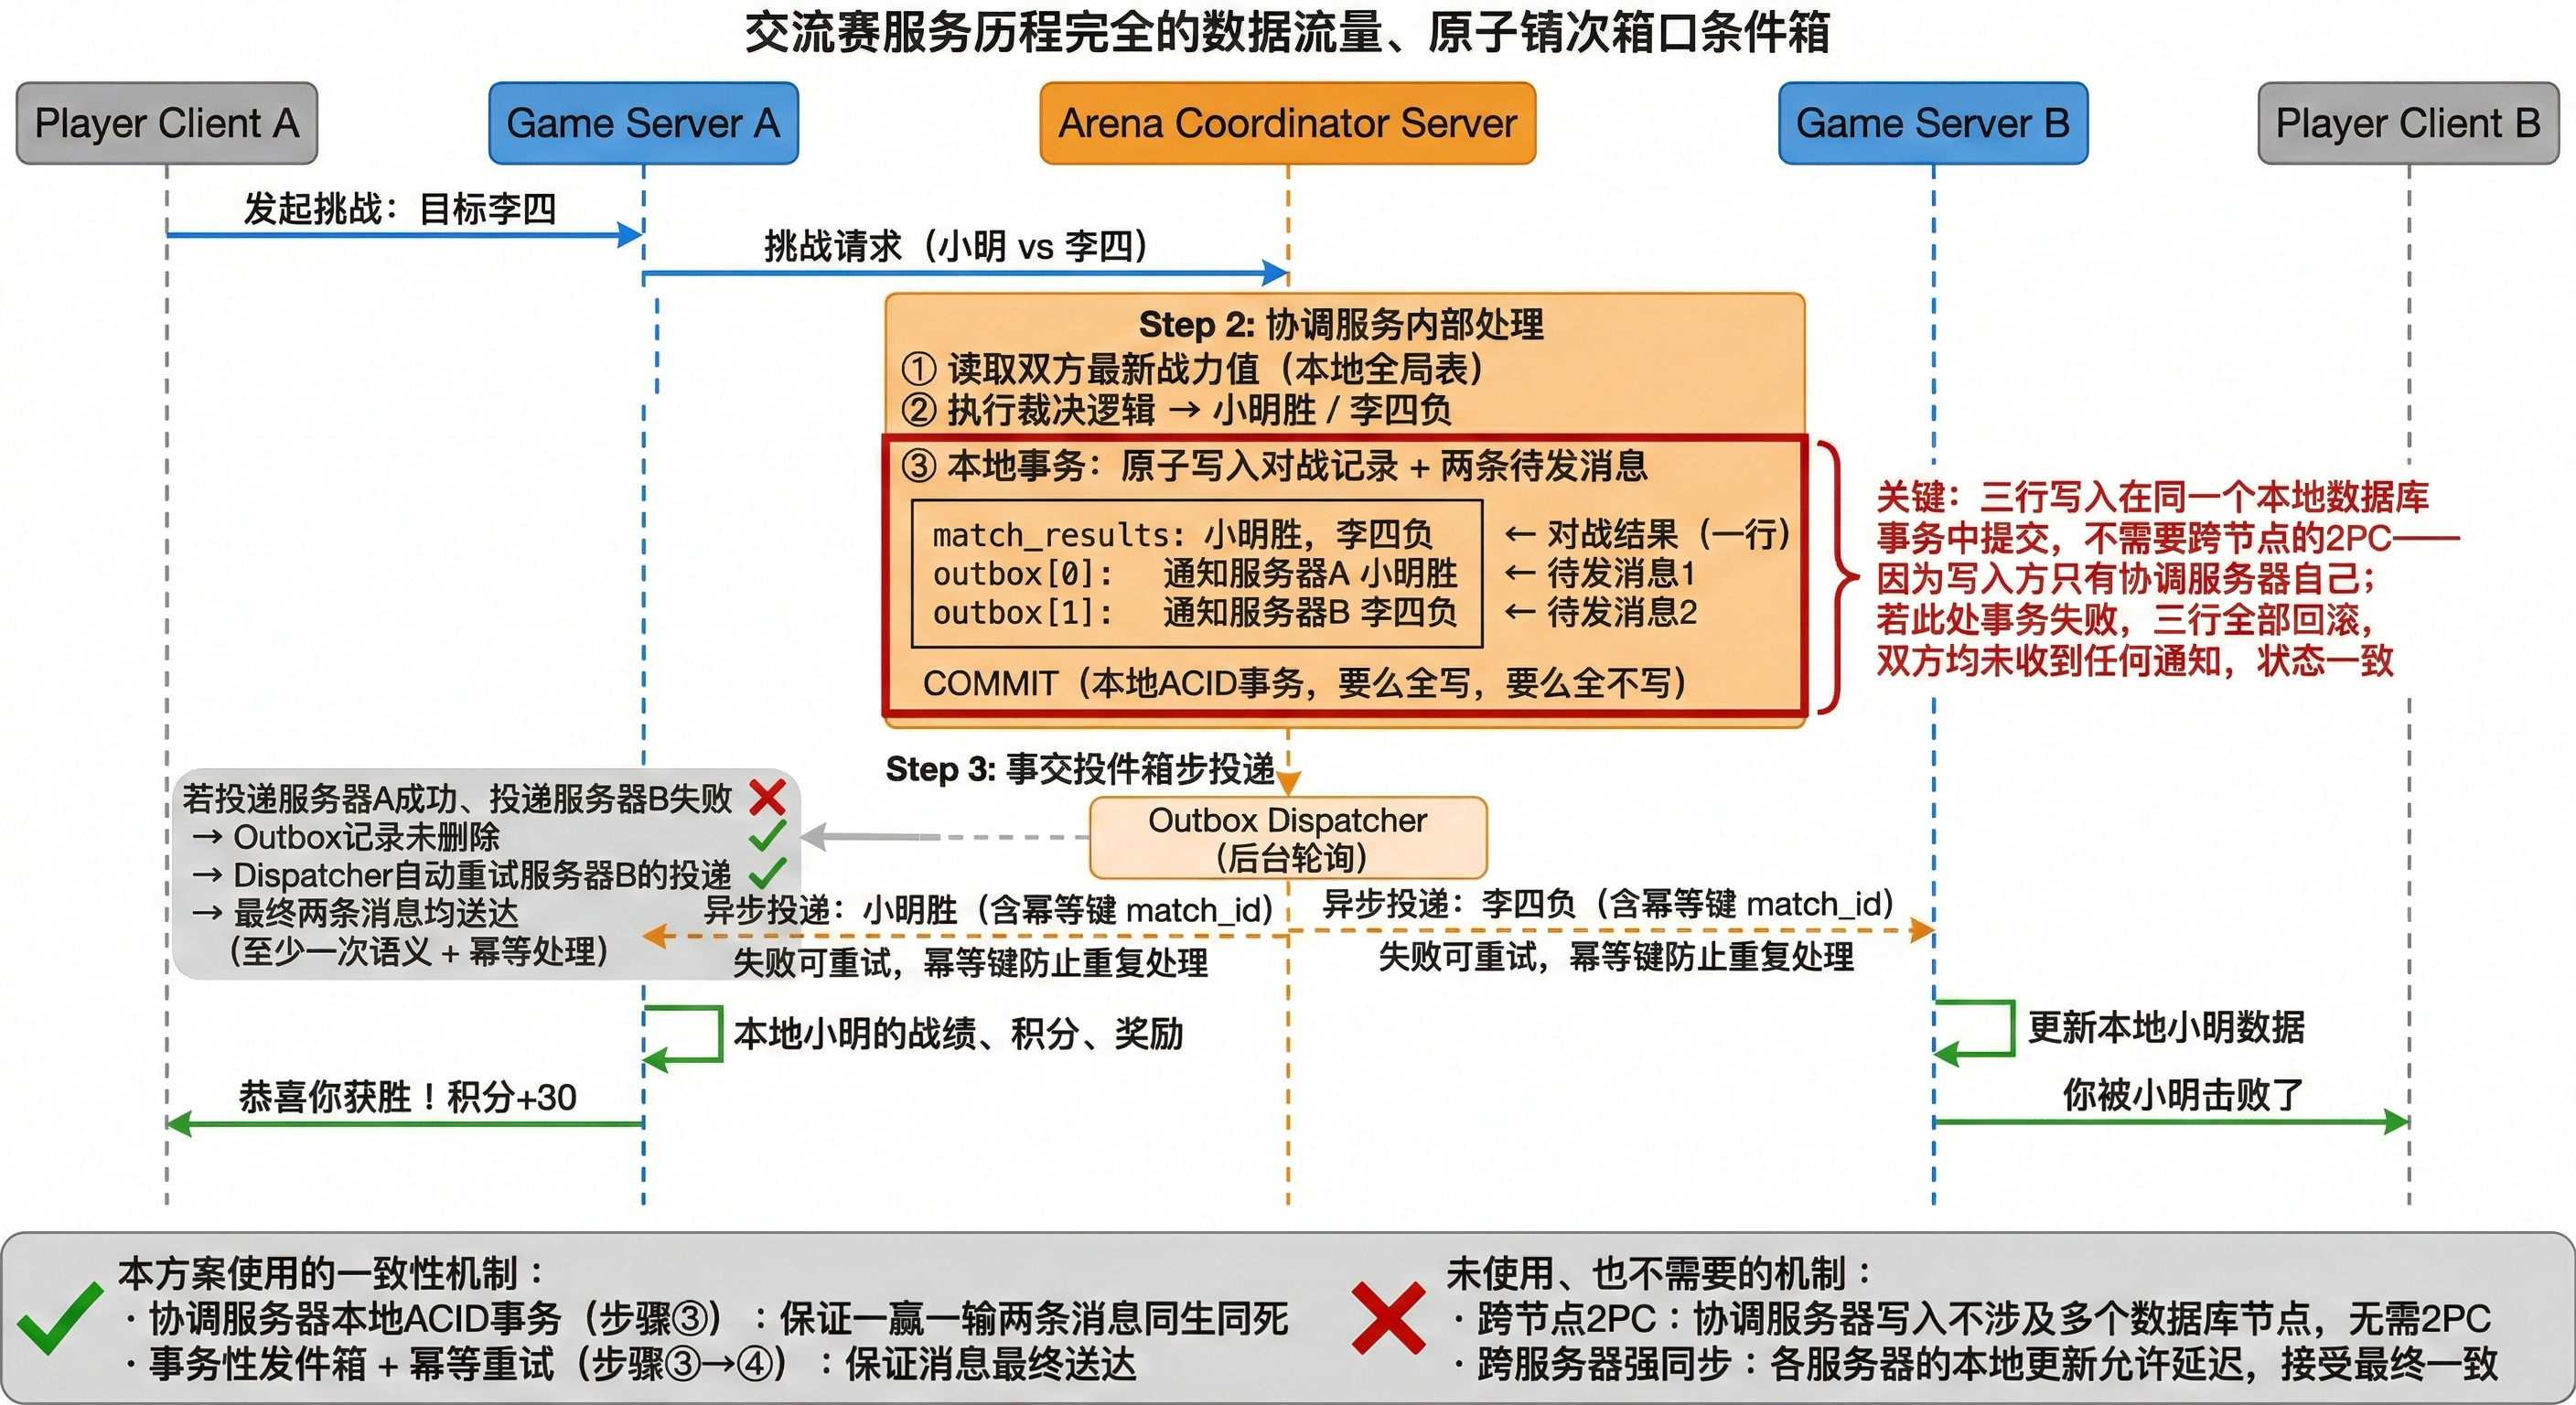
\includegraphics[width=1\linewidth]{figures/sec4/4-5.png}
    \caption{跨服擂台完整数据流：协调服务器以单个本地事务原子写入对战结果与两条待发消息，
    事务性发件箱保证两条消息同生同死，后台 Dispatcher 以幂等重试确保最终送达；
    各游戏服务器的本地战绩更新允许异步延迟，无需跨节点 2PC}
    \label{fig:cross_server_challenge_flow}
\end{figure}


\subsubsection{容错与高可用：协调服务器的挑战}

引入单点裁决解决了一致性问题，但也随之带来了一个新的挑战：
如果擂台协调服务器崩溃了怎么办？
它是整个跨服擂台系统的核心裁决点，一旦宕机，
所有服务器的玩家都无法发起挑战、查询排名、提交报名，整个玩法立刻瘫痪。
因此，协调服务器不能以单台机器的形式存在，
而必须被扩展为一个多节点的高可用集群。
图~\ref{fig:coordinator_cluster_arch} 展示了这个集群在整个跨服擂台系统中的位置：
游戏服务器将所有挑战请求发往集群中当前的 Leader 节点，
Leader 负责裁决并将结果持久化到下方的数据库，
同时通过事务性发件箱将结果异步派发回各游戏服务器；
集群内部的多个节点之间持续同步数据，使得任意一个节点崩溃后，
其他节点都能立刻接管服务。

\begin{figure}[htbp]
    \centering
    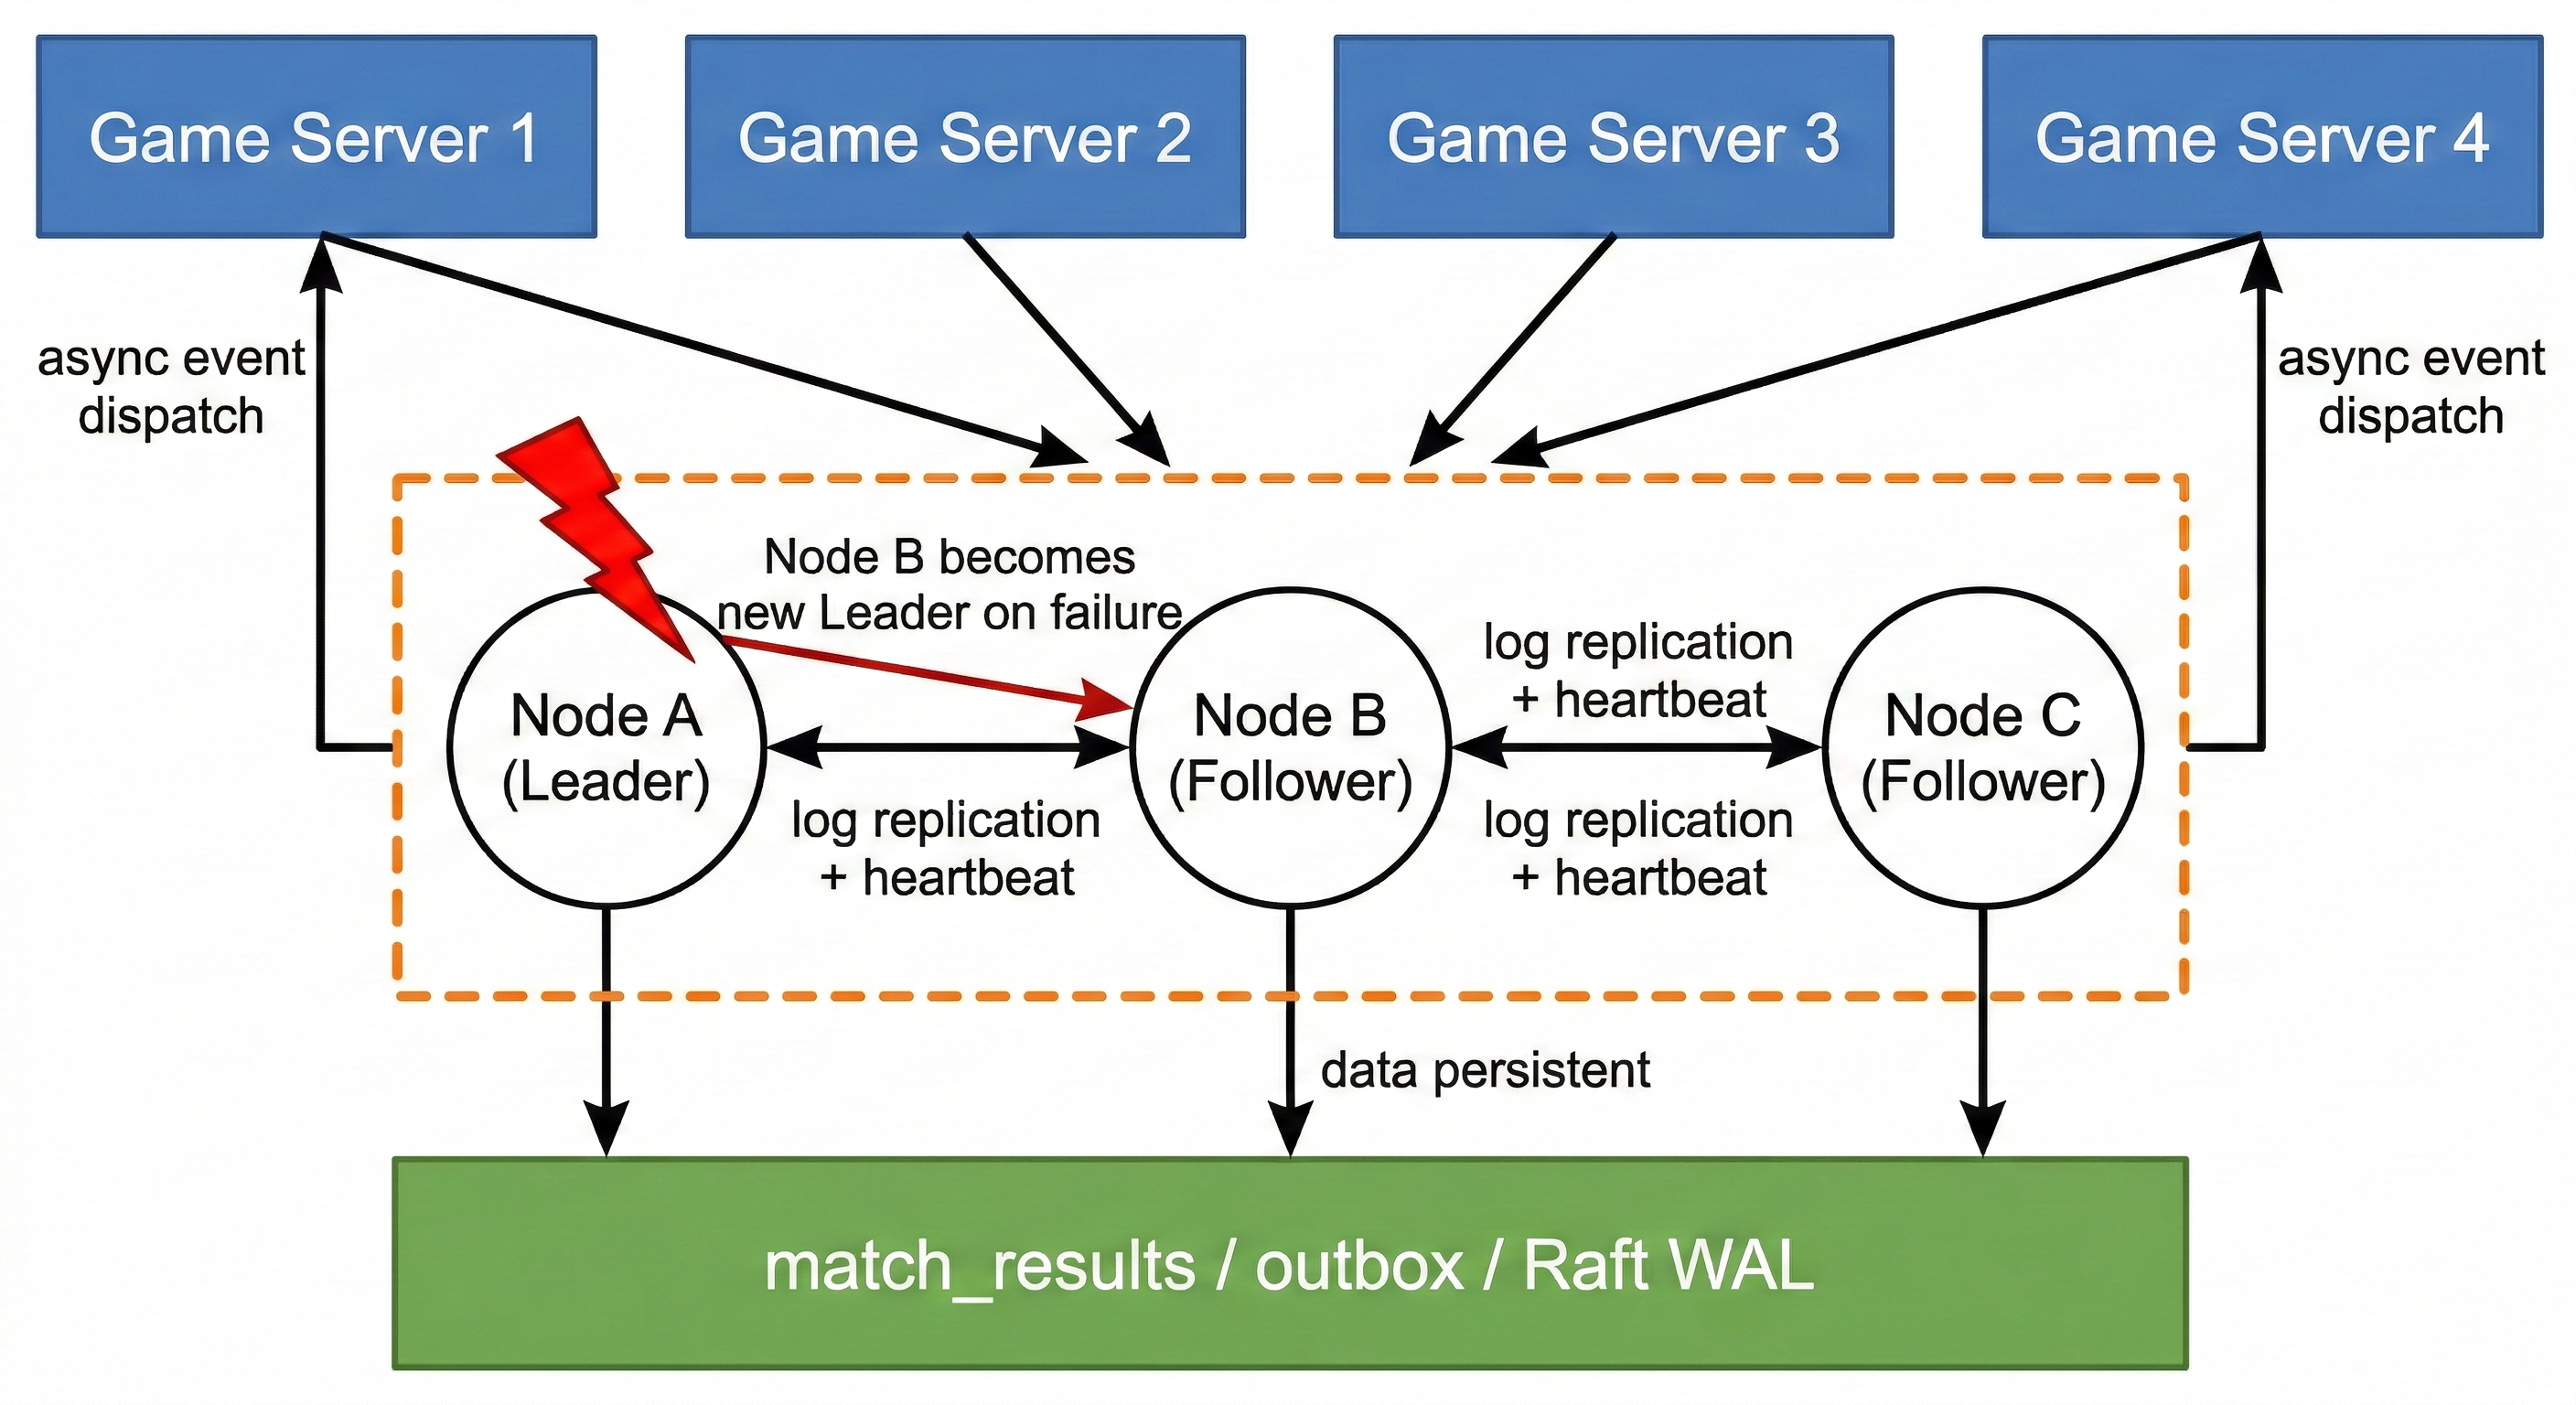
\includegraphics[width=1\linewidth]{figures/sec4/4-coord-arch.png}
    \caption{跨服擂台系统架构：游戏服务器将请求发往协调服务器集群的 Leader，
    集群通过 Raft 协议维护多节点一致性，Leader 崩溃后集群自动选出新 Leader}
    \label{fig:coordinator_cluster_arch}
\end{figure}

构建多节点集群，首先面对的是一个基本问题：集群里谁说了算，以及如何让所有节点
对"操作历史"始终保持一致的认知？这正是分布式系统中经典的共识（Consensus）问题。
Raft 算法由 Diego Ongaro 和 John Ousterhout 于 2014 年提出，
其核心设计目标便是"可理解性"——将共识问题显式地拆解为领导者选举、
日志复制和安全性约束三个子问题分别处理，使得工程师能够清楚地推理系统在各种故障下的行为。

\paragraph{节点角色与任期}

Raft 将集群中的每个节点建模为一个状态机，节点在任意时刻处于三种角色之一：
跟随者（Follower）、候选者（Candidate）或领导者（Leader）。
集群正常运行时只存在一个 Leader，它是唯一接受外部写请求的权威节点；
其余节点均为 Follower，被动接收来自 Leader 的日志和心跳。
Raft 使用单调递增的整数"任期"（Term）来标识时间区段，
每个任期最多只有一个合法的 Leader——这一"任期唯一性"是 Raft
所有安全性保证的出发点。

\paragraph{领导者选举}

每个 Follower 都维护一个随机化的选举超时计时器（通常在 150\,ms 到 300\,ms 之间随机取值）。
若在超时时间内未收到来自 Leader 的心跳，节点就认为当前没有合法的 Leader，
于是将自身切换为 Candidate，将 Term 加一，投票给自己，
并向所有其他节点发送 \texttt{RequestVote} 消息。
其他节点收到投票请求时，须同时满足两个条件才会投赞成票：
候选者的 Term 不小于自身当前的 Term，以及候选者的日志至少和自己一样新
（先比较最后一条日志的任期号，再比较其索引，取较大者为"更新"）。
每个节点在同一 Term 内只能投票给一个候选者。
某个候选者一旦收到超过半数节点的赞成票，即成为新 Leader，
立即向所有节点发送心跳，阻止其他节点再次发起选举。

随机化超时是防止"分票"（Split Vote）僵局的关键。
若所有节点同时超时并发起选举，每人只投自己，无人获得多数票，选举失败需重试。
随机化使得某一个节点几乎总是比其他节点提前超时，
率先收集到足够的选票，在其他节点触发超时之前就完成当选。
图~\ref{fig:raft_core} 左侧展示了一次完整的选举流程：
节点 A 率先超时当选（Term=2），随后 A 崩溃，节点 B 率先超时，
在 Term=3 中收集到 C 的投票后成为新 Leader，
总服务中断时间约等于一次选举超时长度。

\paragraph{日志复制}

Leader 选出之后，外部的每一个写请求都经由以下流程被持久化并执行，
如图~\ref{fig:raft_core} 右侧所示。以"小明挑战李四"为例：
Leader 收到请求后，先将其封装为带有索引和任期号的日志条目追加到本地日志，
此时该条目尚未提交（灰色）；随后 Leader 并发地将该条目通过
\texttt{AppendEntries} 消息复制到所有 Follower。
Follower 收到后先做"前缀匹配检查"——验证消息中携带的前一条日志的索引与任期
是否与自身日志末尾完全吻合，若不吻合则拒绝，Leader 会自动回退重试直到找到对齐点；
检查通过后 Follower 追加条目并回复成功。
当 Leader 收到超过半数节点（含自身）的成功回复后，
该条目被标记为"已提交"（Committed，绿色），
Leader 将其应用到状态机——在擂台场景中即执行裁决逻辑、
以本地 ACID 事务原子写入 \texttt{match\_results} 和 \texttt{outbox}。
此后 Leader 将 \texttt{commitIndex} 通过后续心跳告知所有 Follower，
Follower 也将该条目应用到本地状态机，三个节点最终持有完全相同的日志和状态。

提交只要求多数节点确认而非全部节点，这正是 Raft
能够在节点部分失联时仍然正常工作的根本原因：
三节点集群在一个 Follower 暂时失联时依然可以提交，
失联节点恢复后会自动通过日志同步补全缺失的条目。

\begin{figure}[htbp]
    \centering
    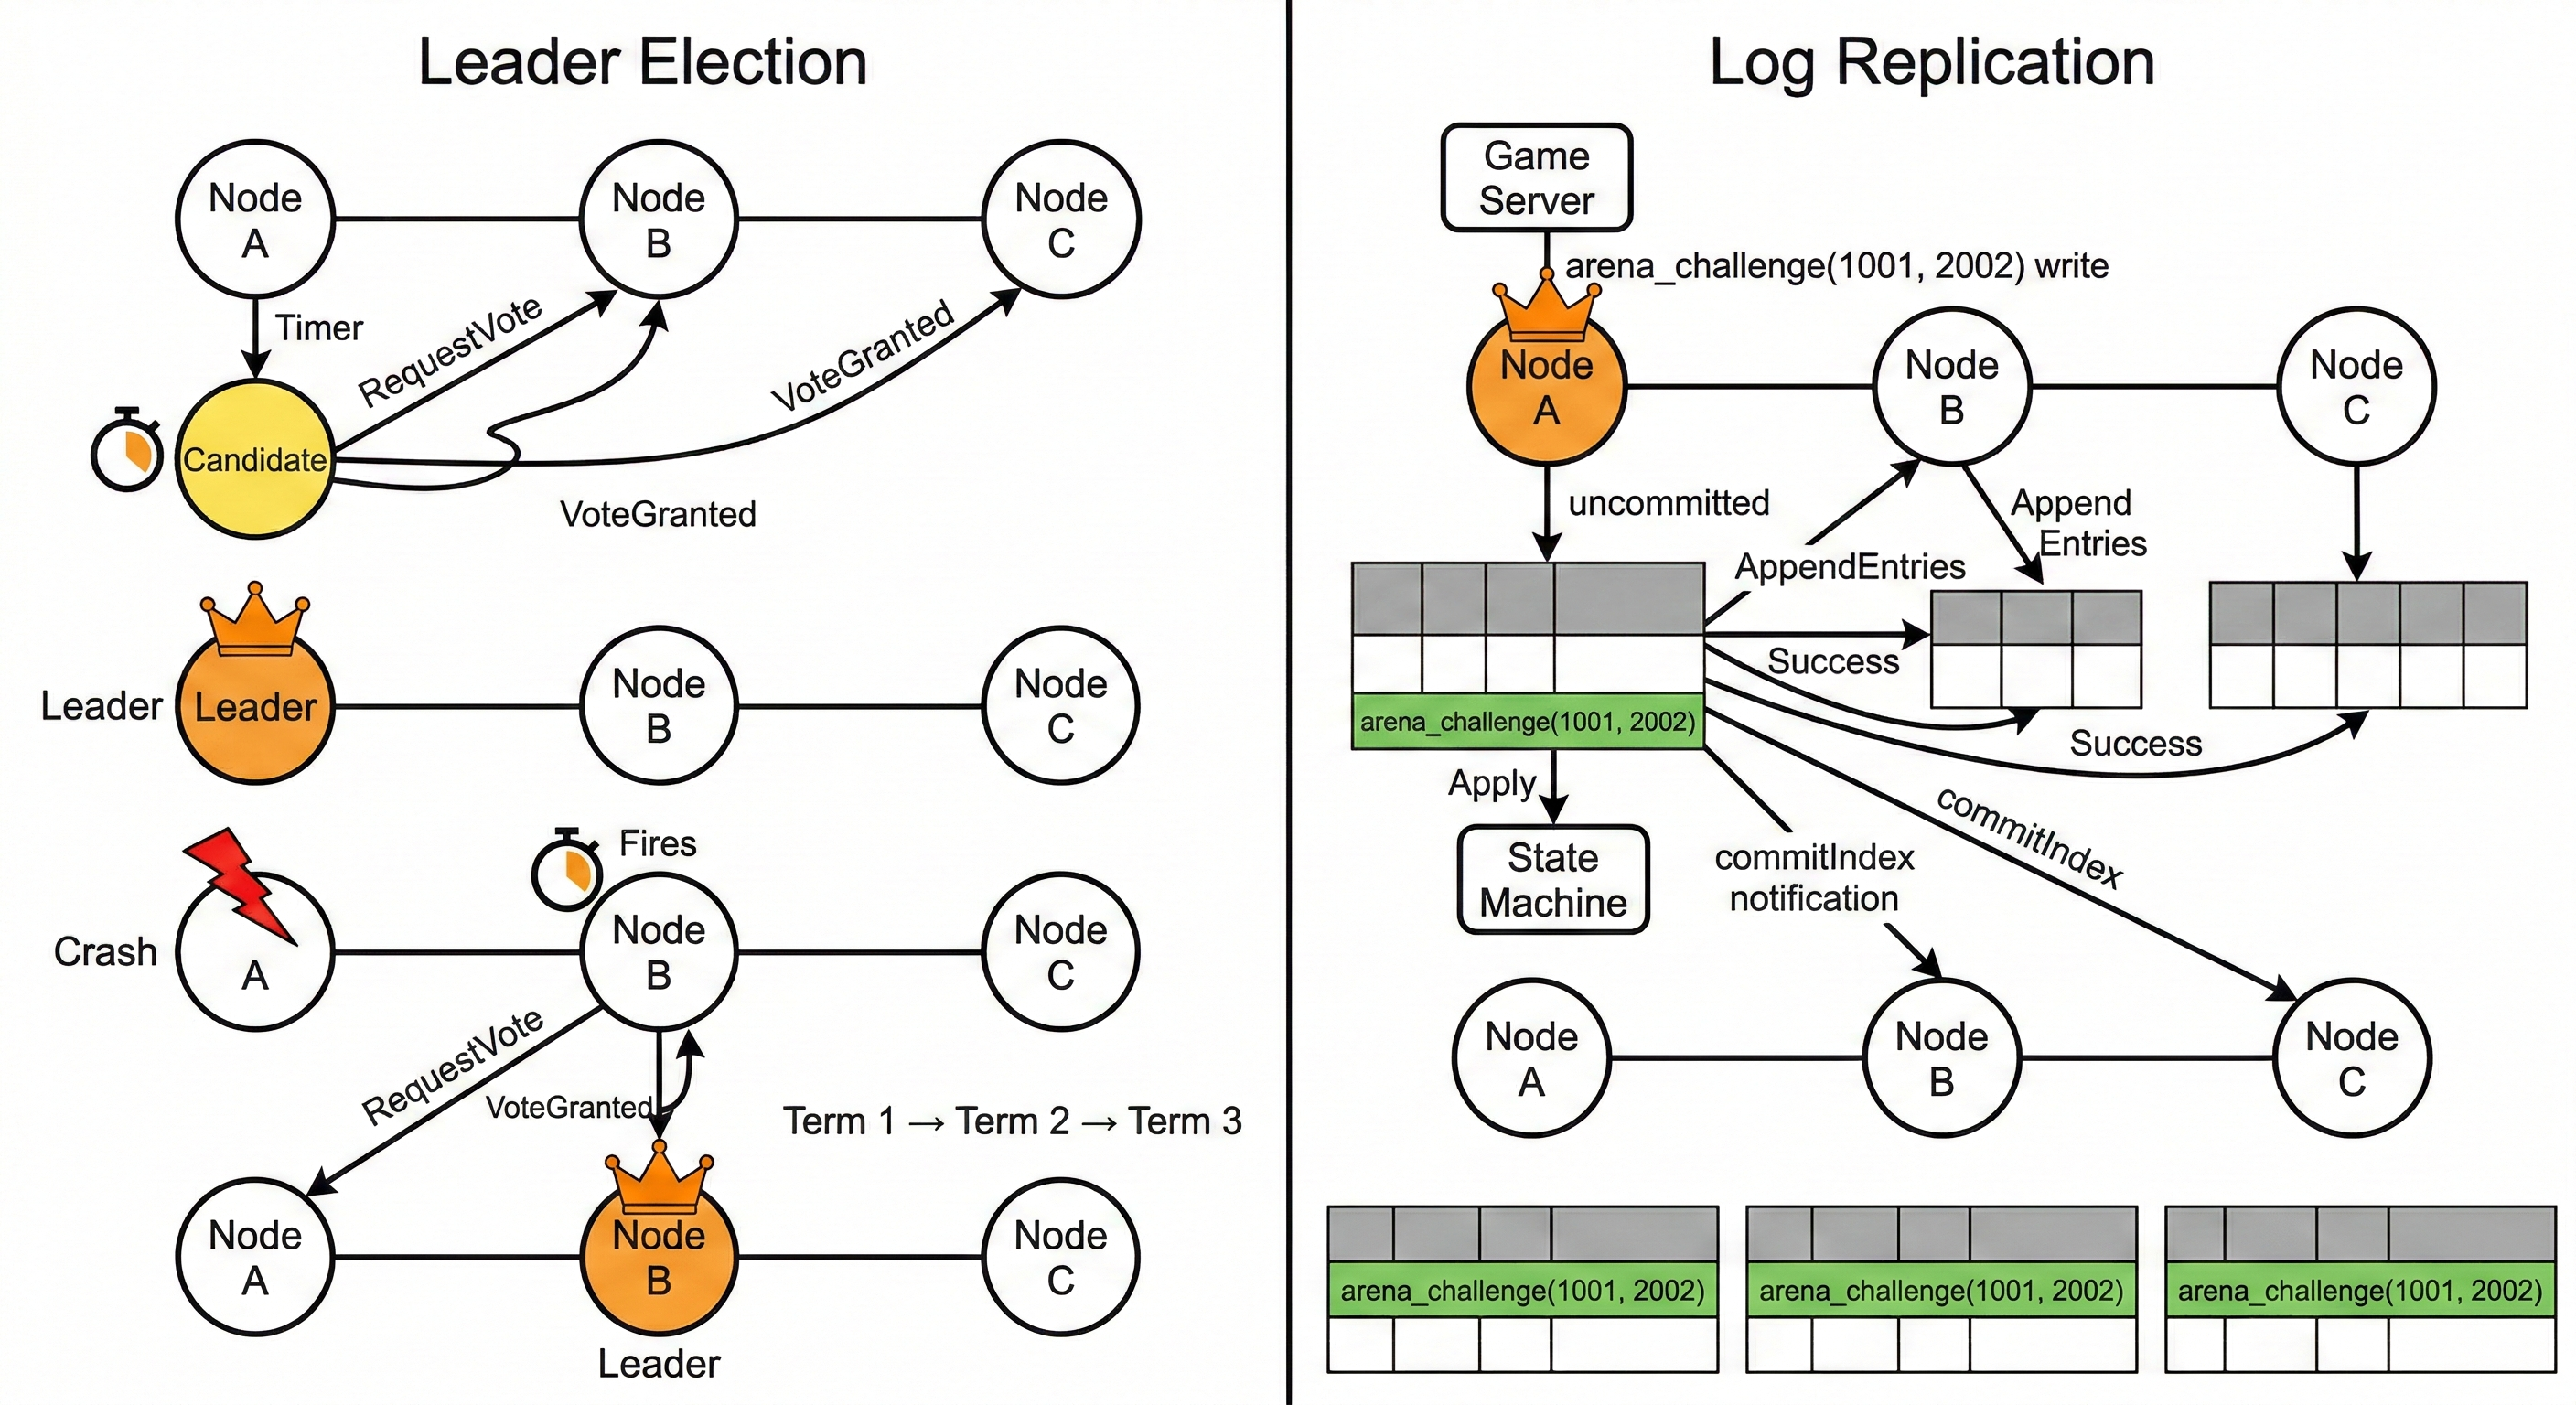
\includegraphics[width=1\linewidth]{figures/sec4/4-raft-core.png}
    \caption{Raft 核心机制（左）领导者选举：随机化超时防止分票，
    Term 单调递增保证不会选出过期节点；
    （右）日志复制：Leader 追加并复制日志，多数确认后提交，
    所有节点状态机最终一致}
    \label{fig:raft_core}
\end{figure}

\paragraph{安全性：为什么已提交的数据不会丢失}

Raft 最核心的安全性保证是：任何已提交的日志条目，
在集群经历任意节点崩溃和重新选举之后，都不会被覆盖或丢失。
这一保证来自选举时"日志最新"的约束。
一条日志条目被提交，意味着它已经存在于集群中超过半数的节点上；
而任何候选者想要当选，也必须获得超过半数节点的投票。
这两个"超过半数"的集合必然存在交集——至少有一个节点同时拥有已提交的条目
且参与了本次投票。该节点只会把票投给"日志至少和自己一样新"的候选者，
这就保证了新 Leader 的日志必然包含所有已提交的条目，
历史数据永不倒退。

\paragraph{集群规模与工程实践}

在实际部署中，协调服务器集群通常选择三节点或五节点配置。
三节点集群可容忍一台服务器同时故障（$\lfloor 3/2 \rfloor = 1$），
适合单机房的普通可用性场景；
五节点集群可容忍两台同时故障（$\lfloor 5/2 \rfloor = 2$），
适合需要跨机房部署或对可用性要求更高的场景。
Raft 日志本身就是持久化的载体：每个节点以 WAL（Write-Ahead Log）的形式
将日志顺序追加写入本地磁盘，崩溃重启后直接回放日志即可恢复状态。
当日志积累过长时，Raft 还支持快照压缩（Snapshotting）：
将当前完整的状态机快照落盘，删除快照之前的全部日志，
防止日志文件无限增长，同时保证新节点加入时能够快速同步状态。


\subsubsection{从简化到扩展：跨服擂台的演进空间}

通过这个完整的跨服擂台案例，我们看到了分布式架构的两个重要价值。第一，它不仅仅是为了"扛住更多人"，还能够支撑单机时代难以实现的玩法创新——只有当玩家被分散到多个服务器上，"跨服"这一概念才有存在的意义，而跨服玩法可以打破服务器壁垒，让所有玩家在一个更大的舞台上竞技，提升游戏的社交性和竞技性。第二，通过刻意简化战斗规则（只比较战力值，不模拟复杂战斗），这个案例让我们能够集中精力理解"协调服务器"、"唯一裁决"、"多服同步"等分布式系统的核心概念。

但简化并不意味着这个架构只能支撑简单的玩法。当我们理解了简化版本的跨服擂台如何工作之后，就可以逐步引入更复杂的战斗机制。例如，可以将战力比拼升级为回合制战斗：协调服务器不再只是比较一个数值，而是模拟多个回合的攻击与防御，每个回合根据双方的攻击力、防御力、技能效果计算伤害，直到某一方血量归零。这种扩展不需要改变整体架构——协调服务器仍然是唯一的裁决点，游戏服务器仍然是代理和执行者，只是裁决逻辑从简单的数值比较变成了多回合的战斗模拟。

进一步地，还可以引入技能释放和战术选择。玩家在挑战时不仅选择对手，还可以选择使用哪些技能、采用什么战术。协调服务器在裁决时会考虑这些因素，比如某个技能对某种类型的敌人有额外伤害，某个战术在先手时更有优势。这时协调服务器的裁决逻辑会更复杂，但核心的架构模式仍然不变——唯一真相源、单点裁决、多点跟随。

甚至可以探索简化的实时对战。虽然完整的实时对战需要高频率的状态同步和低延迟的网络通信，但我们可以设计一种"伪实时"的战斗模式：玩家在挑战时预先设定自己的行动序列（比如"第 1 秒释放技能 A，第 3 秒移动到位置 B，第 5 秒释放技能 C"），提交给协调服务器；协调服务器收集双方的行动序列后，在本地模拟整个战斗过程，计算每个时刻双方的位置、血量、技能冷却等状态，最终给出战斗结果和完整的战斗回放。这种模式虽然不是真正的实时对战，但可以给玩家带来类似实时对战的体验，同时又避免了实时同步的复杂性和网络延迟的影响。

无论如何扩展，跨服擂台的核心设计原则始终不变：将全局状态集中在一个权威的协调服务器上，让各个游戏服务器只负责代理和执行，通过清晰的职责划分和单向的数据流，保证分布式环境下的一致性和正确性。这种设计模式不仅适用于擂台，也适用于任何需要跨服交互的玩法——跨服副本、跨服拍卖行、跨服公会战等，都可以借鉴这个架构思路，根据具体的业务需求调整协调逻辑和交互流程。

\subsection{小结：集中到分布}

本章系统讲解了游戏服务器从单机架构到多机分布式架构的完整演进路径。我们首先学习了数据库分片技术，理解了如何通过选择合适的分片键和分配策略，将原本集中在单一数据库中的玩家数据分散到多台独立的数据库实例上，从而突破单机存储容量的天花板。在这个过程中，我们也认识到了分片带来的挑战，包括跨分片查询的效率问题和跨分片事务的复杂性，学会了如何通过业务设计——如异步化处理、数据模型重组、容忍最终一致性——来规避这些问题，避免陷入分布式事务的泥潭。

接下来，我们学习了负载均衡的基本原理和常见策略。从最简单的轮询分配，到基于实时状态的最少连接策略，再到引入加权负载评估、动态权重调整、健康检查机制、运行时动态迁移，我们逐步理解了如何将玩家流量合理分配到各个游戏服务器上，确保每台服务器都处于相对均衡的工作状态。负载均衡不是某一个具体的算法，而是一整套围绕"合理使用每一份资源"展开的系统性思考——它需要实时监控各服务器的状态，需要根据硬件配置动态调整权重，需要及时发现和隔离故障节点，需要在运行时灵活迁移玩家以应对突发负载。

最后，我们通过跨服擂台这个实战案例，学习了在分布式环境下不同服务器间如何进行玩家交互与状态同步。通过引入擂台协调服务器作为唯一的裁决点，我们成功实现了来自不同服务器的玩家在统一平台上的公平竞技。这个案例展示了"单点裁决、多点跟随"这一分布式系统的核心设计模式：全局状态由一个权威的协调服务器维护，各个游戏服务器只负责代理玩家的请求和执行协调服务器的指令，不做独立的裁决，从而避免了"双重历史"导致的数据不一致。同时，我们也看到了如何通过刻意简化业务规则（只比较战力值，不模拟复杂战斗），将注意力集中在分布式协调的核心问题上，为后续学习更复杂的分布式协作机制奠定基础。

%从单机到多机的演进，本质上是从"集中式"到"分布式"的架构升级。本章介绍的数据分片、负载均衡、跨服通信等技术，构成了分布式游戏服务器的基础架构体系。
%在下一章中，我们将进一步深入分布式系统的核心问题：当多台服务器需要就某一个全局状态达成共识时，如何在网络延迟、节点故障、并发冲突等复杂条件下，仍然能够保证系统的正确性与可用性。

\newpage
